\documentclass[11pt]{book}

\tolerance=600

% for \begin{center}, etc.
\usepackage[margin=1.0in]{geometry}

\usepackage{seqsplit}

% all kinds of math macros
\usepackage{amsmath}
\usepackage{amssymb}

% eps figures
\usepackage{epsfig}

% chapter title styles
\usepackage[Sonny]{fncychap}
\ChNameVar{\LARGE}
\ChTitleVar{\LARGE\sl}

% index
\usepackage{makeidx}
\makeindex


% part page style see
% http://tex.stackexchange.com/questions/6609/problems-with-part-labels-using-titlesec
\usepackage{titlesec}

\titleformat{\part}[display]
   {\Huge\filcenter}
   {{\partname{}} \thepart}
   {0em}
   {\hrule}



% hyperlinks -- load after fncychap
\usepackage{hyperref}

% color package
\usepackage[usenames]{color}

% longtable package used to split tables across pages
\usepackage{longtable}

% PDF-aware landscape package, used for rotating tables (including the
% longtable)
\usepackage{pdflscape}

% table coloring
\usepackage{colortbl}
\definecolor{tableShade}{rgb}{0.945,0.961,0.980}

% caption
\usepackage{caption}
\captionsetup[figure]{font=small,labelfont=small}

% make the MarginPars look pretty
\setlength{\marginparwidth}{0.75in}
\newcommand{\MarginPar}[1]{\marginpar{\vskip-\baselineskip\raggedright\tiny\sffamily
\hrule\smallskip{\color{red}#1}\par\smallskip\hrule}}

% to increase the likelihood that floats will occur "here" when you
% want them to
\renewcommand{\floatpagefraction}{1.0}
\renewcommand{\topfraction}{1.0}
\renewcommand{\bottomfraction}{1.0}
\renewcommand{\textfraction}{0.0}

% number subsubsections and put them in the TOC
\setcounter{tocdepth}{3}
\setcounter{secnumdepth}{3}

% custom hrule for title page
\newcommand{\HRule}{\rule{\linewidth}{0.125mm}}

% control sequences in verbatim
\usepackage{fancyvrb}

% short table of contents
\usepackage{shorttoc}

% spacing in the table of contents
\usepackage[titles]{tocloft}

\setlength{\cftbeforechapskip}{2ex}
\setlength{\cftbeforesecskip}{0.25ex}

% For splitting up lists into multitple columns
\usepackage{multicol}

% don't put a header on blank pages, see
% http://www.latex-community.org/forum/viewtopic.php?f=4&p=51559
% change ``plain'' to ``empty'' to eliminate the page number
\makeatletter
\renewcommand*\cleardoublepage{\clearpage\if@twoside
\ifodd\c@page\else
\hbox{}
\thispagestyle{empty}
\newpage
\if@twocolumn\hbox{}\newpage\fi\fi\fi}
\makeatother


% don't make the chapter/section headings uppercase.  See the fancyhdr
% documentation (section 9)
\usepackage{fancyhdr}
\renewcommand{\chaptermark}[1]{%
 \markboth{\chaptername
\ \thechapter.\ #1}{}}

\renewcommand{\sectionmark}[1]{\markright{\thesection---#1}}


% skip a bit of space between paragraphs, to enhance readability
\usepackage{parskip}



% special fraction
\newcommand{\sfrac}[2]{\mathchoice
  {\kern0em\raise.5ex\hbox{\the\scriptfont0 #1}\kern-.15em/
   \kern-.15em\lower.25ex\hbox{\the\scriptfont0 #2}}
  {\kern0em\raise.5ex\hbox{\the\scriptfont0 #1}\kern-.15em/
   \kern-.15em\lower.25ex\hbox{\the\scriptfont0 #2}}
  {\kern0em\raise.5ex\hbox{\the\scriptscriptfont0 #1}\kern-.2em/
   \kern-.15em\lower.25ex\hbox{\the\scriptscriptfont0 #2}}
  {#1\!/#2}}

\def\Ab {{\bf A}}
\def\eb {{\bf e}}
\def\Fb {{\bf F}}
\def\gb {{\bf g}}
\def\Hb {{\bf H}}
\def\ib {{\bf i}}
\def\Ib {{\bf I}}
\def\Kb {{\bf K}}
\def\lb {{\bf l}}
\def\Lb {{\bf L}}
\def\nb {{\bf n}}
\def\Pb {{\bf P}}
\def\Qb {{\bf Q}}
\def\rb {{\bf r}}
\def\Rb {{\bf R}}
\def\Sb {{\bf S}}
\def\ub {{\bf u}}
\def\Ub {{\bf U}}
\def\xb {{\bf x}}

\def\dt       {\Delta t}
\def\omegadot {\dot\omega}

\def\inp  {{\rm in}}
\def\outp {{\rm out}}
\def\sync {{\rm sync}}

\def\half   {\frac{1}{2}}
\def\myhalf {\sfrac{1}{2}}
\def\nph    {{n+\myhalf}}

% Level Set Macros
\def\ADDNODE       {{\tt{\bf ADDNODE}}}
\def\ADVANCE       {{\tt{\bf ADVANCE}}}
\def\done          {{\tt{\bf done}}}
\def\EVAL          {{\tt{\bf EVAL}}}
\def\INITPHI       {{\tt{\bf INITPHI}}}
\def\FASTMARCH     {{\tt{\bf FASTMARCH}}}
\def\FINDINTRFCE   {{\tt{\bf FINDINTRFCE}}}
\def\heap          {{\tt{\bf heap}}}
\def\heaploc       {{\tt{\bf heaploc}}}
\def\intface       {{\tt{\bf intface}}}
\def\intfacen      {{\tt{\bf intfacen}}}
\def\intfacenum    {{\tt{\bf intfacenum}}}
\def\intfacenumn   {{\tt{\bf intfacenumn}}}
\def\intfacenump   {{\tt{\bf intfacenump}}}
\def\intfacep      {{\tt{\bf intfacep}}}
\def\isnew         {{\tt{\bf isnew}}}
\def\LARGEINT      {{\tt{\bf LARGEINT}}}
\def\lvlerr        {{\tt{\bf lvlerr}}}
\def\LSCFL         {{\tt{\bf LSCFL}}}
\def\LStype        {{\tt{\bf LStype}}}
\def\LSnband       {{\tt{\bf LSnband}}}
\def\LSmine        {{\tt{\bf LSmine}}}
\def\mine          {{\tt{\bf mine}}}
\def\MINE          {{\tt{\bf MINE}}}
\def\mineloc       {{\tt{\bf mineloc}}}
\def\NARROWBAND    {{\tt{\bf NARROWBAND}}}
\def\nband         {{\tt{\bf nband}}}
\def\nbandnum      {{\tt{\bf nbandnum}}}
\def\nbandwidth    {{\tt{\bf nbandwidth}}}
\def\numtent       {{\tt{\bf numtent}}}
\def\PHIUPD        {{\tt{\bf PHIUPD}}}
\def\REINIT        {{\tt{\bf REINIT}}}
\def\RETYPIFY      {{\tt{\bf RETYPIFY}}}
\def\RMVNODE       {{\tt{\bf RMVNODE}}}
\def\sign          {{\tt{\bf sign}}}
\def\type          {{\tt{\bf type}}}
\def\UPDATE        {{\tt{\bf UPDATE}}}
\def\UPDATEF       {{\tt{\bf UPDATEF}}}
\def\UPDATENODE    {{\tt{\bf UPDATENODE}}}
\def\new           {{\rm new}}
\def\old           {{\rm old}}


\usepackage{listings}

\usepackage{subfig}

\definecolor{gray}{rgb}       {0.8,0.8,0.8}
\definecolor{light-blue}{rgb} {0.8,0.8,1.0}
\definecolor{light-green}{rgb}{0.8,1.0,0.8}
\definecolor{light-red}{rgb}  {1.0,0.9,0.9}

\lstset{frame=single,basicstyle=\footnotesize\ttfamily,showstringspaces=false,showspaces=false,xleftmargin=5pt,xrightmargin=6pt}

\lstset{language=C++,
                basicstyle=\footnotesize\ttfamily,
                keywordstyle=\color{blue}\footnotesize\ttfamily,
                commentstyle=\color{cyan}\footnotesize\ttfamily
}

\lstdefinelanguage{cpp}{
  language     = C++,
  morekeywords =
  [2]{amrex,amrex_real,
      Array,BaseFab,Box,BoxArray,DistributionMapping,FabArray,FArrayBox,
      Geometry,IArrayBox,IntVect,IndexType,MFIter,MultiFab,
      ParallelDescriptor,ParmParse,Real,RealBox,
      AMREX_SPACEDIM,AMREX_D_DECL},
  keywordstyle = [2]\color{red}\footnotesize\ttfamily,
}

% \lstset{
%   basicstyle=\small\ttfamily,%
%   frame=single,%
%   rulesepcolor=\color{gray},%
%   backgroundcolor=\color{white}%
% }
% \lstset{belowskip=-0.25em}


% Macros for indexing
\newcommand{\idxamrex}[1]{\index{\tt{amrex}!{\tt #1}}{\tt #1}}

%------------------------------------------------------------------------------
\input amrexsymbols
% \graphicspath{{Verification/}{Software/}{ConvertCheckpoint/}{Scaling/}{Visualization/}}


%------------------------------------------------------------------------------
\begin{document}



\frontmatter

\begin{titlepage}
\begin{center}
\ \\[3in]
{\sf \Huge AMReX}
\ \\[0.2in]

\begin{minipage}{5.5in}
\HRule\\[2mm]
\centering
{\Large \em An adaptive mesh refinement software framework}

\HRule
\end{minipage}

\ \\[.5 in]
{\sf \huge User's Guide}

\vfill

{\large AMReX Developers}
\ \\[0.3 in]
{\large \today}
\end{center}

\end{titlepage}


\shorttoc{Chapter Listing}{0}

\setcounter{tocdepth}{2}
\tableofcontents

\clearpage

\listoffigures
\addcontentsline{toc}{chapter}{list of figures}

\clearpage

\listoftables
\addcontentsline{toc}{chapter}{list of tables}


\cleardoublepage

\chapter*{Preface}
\addcontentsline{toc}{chapter}{Preface}
\input{Preface/Preface}

\mainmatter

\chapter{Introduction}\label{Chap:Introduction}
\amrex\ is a publicly available software framework designed for
building massively parallel block-structured adaptive mesh refinement
(AMR) applications.

Key features of \amrex\ include:
\begin{itemize}
\item \cpp\ and Fortran interfaces
\item 1-, 2- and 3-D support
\item Support for cell-centered, face-centered, edge-centered, and
  nodal data
\item Support for hyperbolic, parabolic, and elliptic solves on
  hierarchical adaptive grid structure
\item Optional subcycling in time for time-dependent PDEs
\item Support for particles
\item Parallelization via flat MPI, OpenMP, hybrid MPI/OpenMP, or MPI/MPI
\item Parallel I/O
\item Plotfile format supported by \amrvis, \visit, \paraview, and \yt.
\end{itemize}

Because \amrex's core is mainly written in \cpp, the basics of \amrex\
is first introduced in \cpp\ and then their Fortran wrappers if
available will be described as well.  

Besides the User's Guide, there is document generated by Doxygen at
\url{https://ccse.lbl.gov/pub/AMReX_Docs/}.  Documentation on
migration from \boxlib\ is available at {\tt Docs/Migration}.


\chapter{Getting Started}\label{Chap:GettingStarted}
In this chapter, we will walk you through two simple examples.  It is
assumed here that your machine has GNU Make, Python, GCC (including
gfortran), and MPI, although \amrex\ can be built with CMake and other
compilers. 

\section{Downloading the Code}

The source code of \amrex\ is available at
\url{https://github.com/AMReX-Codes/amrex}.  The GitHub repo is our
central repo for development.  The {\tt development} branch
includes the latest state of the code, and it is merged into the {\tt
  master} branch on a monthly basis.  The {\tt master} branch is
considered the release branch.  The releases are tagged with version
number {\tt YY.MM} (e.g., {\tt 17.04}).  The {\tt MM} part of the
version is incremented every month, and the {\tt YY} part every year.
Bug fix releases are tagged with {\tt YY.MM.patch} (e.g., {\tt
  17.04.1}).

\section{Example: Hello World}

The source code of this example is at {\tt
  amrex/Tutorials/Basic/HelloWorld\_C/} and is also shown below. 

\begin{lstlisting}[language=cpp]
 #include <AMReX.H>
 #include <AMReX_Print.H>

 int main(int argc, char* argv[])
 {
     amrex::Initialize(argc,argv);
     amrex::Print() << "Hello world from AMReX version " 
                    << amrex::Version() << "\n";
     amrex::Finalize();
 }
\end{lstlisting}

The main body of this short example contains three statements.
Usually the first and last statements for the {\tt main} function of
every program should be calling {\tt amrex::}\idxamrex{Initialize} and
\idxamrex{Finalize}, respectively.  The second statement calls {\tt
  amrex::}\idxamrex{Print} to print out a string that includes the
\amrex\ version returned by the {\tt amrex::}\idxamrex{Version}
function.  The example code includes two \amrex\ header files.  Note
that the name of all \amrex\ header files starts with {\tt AMReX\_}
(or just {\tt AMReX} in the case of {\tt AMReX.H}).  All \amrex\
\cpp\ functions are in the {\tt amrex} namespace.  

\subsection{Building the Code}

You build the code in the {\tt amrex/Tutorials/Basic/HelloWorld\_C/}
directory.  Typing {\tt make} will start the compilation process and
result in an executable named {\tt main3d.gnu.DEBUG.ex}.  The name
shows that the GNU compiler with debug options set by \amrex\ is used.
It also shows that the executable is built for 3D.  Although this
simple example code is dimension independent, the dimension matters
for all non-trivial examples.  The build process can be adjusted by
modifying the {\tt amrex/Tutorials/Basic/HellWorld\_C/GNUmakefile} file.
More details on how to build \amrex\ can be found in
Chapter~\ref{Chap:BuildingAMReX}.

\subsection{Running the Code}

The example code can be run as follows,
\begin{verbatim}
  ./main3d.gnu.DEBUG.ex
\end{verbatim}
The result may look like,
\begin{verbatim}
  Hello world from AMReX version 17.05-30-g5775aed933c4-dirty
\end{verbatim}
The version string means the current commit {\tt 5775aed933c4} (note
that the first letter {\tt g} in {\tt g577..} is not part of the hash)
is based on {\tt 17.05} with 30 additional commits and the \amrex\
work tree is dirty (i.e. there are uncommitted changes).

\subsection{Parallelization}

Now let's build with MPI by typing {\tt make USE\_MPI=TRUE}.  This
should make an executable named {\tt main3d.gnu.DEBUG.MPI.ex}.  Note
{\tt MPI} in the file name.  You can then run,
\begin{verbatim}
  mpiexec -n 4 ./main3d.gnu.DEBUG.MPI.ex
\end{verbatim}
The result may look like,
\begin{verbatim}
  MPI initialized with 4 MPI processes
  Hello world from AMReX version 17.05-30-g5775aed933c4-dirty
\end{verbatim}

If the compilation fails, you are referred to
Chapter~\ref{Chap:BuildingAMReX} on how to configure the build
system.

\section{Example: Heat Equation Solver}\label{sec:heat equation}

We now look at a more complicated example at {\tt
  amrex/Tutorials/Basic/HeatEquation\_EX1\_C} and show how simulation
results can be visualized.  Don't worry about the details of the code.
You will be able to understand the code in this example after
Chapter~\ref{Chap:Basics}. 

\subsection{Building and Running the Code}

To build a 2D executable, type {\tt make DIM=2}.  This will generate
an executable named {\tt main2d.gnu.ex}.  To run it, type,
\begin{verbatim}
  ./main2d.gnu.DEBUG.ex inputs_2d
\end{verbatim}
Note that the command takes a file {\tt inputs\_2d}.  When the run
finishes, you will have a number of plotfiles, {\tt plt00000}, {\tt
  plt01000}, etc.  The calculation solves the heat equation in 2D on a
$256 \times 256$ cells domain.  It runs $10,000$ steps and makes a
plotfile every $1,000$ steps.  These are runtime parameters that can
be adjusted in {\tt inputs\_2d}.

\section{Visualization}
There are several visualization tools that can be used for \amrex\
plotfiles.  The standard tool used within the
\amrex-community is \amrvis, a package developed and supported 
by CCSE that is designed specifically for highly efficient visualization
of block-structured hierarchical AMR data.
Plotfiles can also be viewed using the \visit, \paraview, and \yt\ packages.
Particle data can be viewed using \paraview.
Refer to Chapter \ref{Chap:Visualization} for how to use each of these tools.


\chapter{Building AMReX}\label{Chap:BuildingAMReX}

In this chapter, we discuss \amrex's build systems.  There are three
ways to use \amrex.  The approach used by \amrex\ developers uses GNU
Make.  There is no installation step in this approach.  Application
codes adopt \amrex's build system and compile \amrex\ while compiling
their own codes.  This will be discussed in more detail in
Section~\ref{sec:build:make}.  The second approach is to build \amrex\
into a library and install it (Section~\ref{sec:build:lib}).  Then an
application code uses its own build system and links \amrex\ as an
external library.  \amrex\ can also be built with Cmake
(Section~\ref{sec:build:cmake}).

\section{Building with GNU Make}
\label{sec:build:make}

In this build approach, you write your own make files defining a
number of variables and rules.  Then you invoke {\tt make} to start
the building process.  This will result in an executable upon
successful completion.  The temporary files generated in the building
process are stored in a temporary directory named {\tt
  tmp\_build\_dir}.

\subsection{Dissecting a Simple Make File}

An example of building with GNU Make can be found in {\tt
  amrex/Tutorials/Basic/HelloWorld\_C}.  Table~\ref{tab:makevarimp}
shows a list of important variables.
\begin{table}[t]
  \centering
  \begin{tabular}{lcc}
    Variable & Value & Default \\
    \hline
    {\tt AMREX\_HOME} & Path to amrex & environment \\
    {\tt COMP} & {\tt gnu}, {\tt cray}, {\tt ibm}, {\tt intel}, {\tt llvm}, or {\tt pgi} & none \\
    {\tt DEBUG} & {\tt TRUE} or {\tt FALSE} & {\tt TRUE} \\
    {\tt DIM} & 1 or 2 or 3 & none \\
    {\tt USE\_MPI} & {\tt TRUE} or {\tt FALSE} & {\tt FALSE} \\
    {\tt USE\_OMP} & {\tt TRUE} or {\tt FALSE} & {\tt FALSE} \\
    \hline
  \end{tabular}
  \caption{\label{tab:makevarimp} Important make variables}
\end{table}

At the beginning of {\tt
  amrex/Tutorials/Basic/HelloWorld\_C/GNUmakefile}, {\tt AMREX\_HOME}
is set to the path to the top directory of \amrex.  Note that in the
example {\tt ?=} is a conditional variable assignment operator that
only has an effect if {\tt AMREX\_HOME} has not been defined
(including in the environment).  One can also set {\tt AMREX\_HOME} 
as an environment variable.  For example in bash, 
one can set {\tt export AMREX\_HOME=/path/to/amrex}; in tcsh one can set
{\tt setenv AMREX\_HOME /path/to/amrex}.

One must set the {\tt COMP} variable to choose a compiler.  Currently
the list of supported compilers includes {\tt gnu}, {\tt cray}, {\tt
  ibm}, {\tt intel}, {\tt llvm}, and {\tt pgi}.  One must also set the
{\tt DIM} variable to either 1, 2, or 3, depending on the
dimensionality of the problem.

Variables {\tt DEBUG}, {\tt USE\_MPI} and {\tt USE\_OMP} are optional
with default set to {\tt TRUE}, {\tt FALSE} and {\tt FALSE},
respectively.  The meaning of these variables should be obvious.  
When {\tt DEBUG = TRUE}, aggressive compiler optimization flags are turned
off and assertions in \amrex\ source code are turned on.  For
production runs, {\tt DEBUG} should be set to {\tt FALSE}.

After defining these make variables, a number of files, {\tt
  Make.defs}, {\tt Make.package} and {\tt Make.rules}, are included in
{\tt GNUmakefile}.  \amrex\-based applications do not need to include
all directories in \amrex; an application which does not use particles,
for example, does not need to include files from the {\tt Particle}
directory in its build.
In this simple example, we only need to include {\tt
  \$(AMREX\_HOME)/Src/Base/Make.package}.  An application code also
has its own {\tt Make.package} file (e.g., {\tt ./Make.package} in
this example) to append source files to the build system using
operator {\tt +=}.  Variables for various source files are shown
below.
\begin{quote}
\begin{description}
\item [{CEXE\_sources}] \cpp\ source files.  Note that \cpp\
  source files are assumed to have a {\tt .cpp} extension.
\item [{CEXE\_headers}] \cpp\ headers with {\tt .h} or {\tt .H} extension.
\item [{cEXE\_sources}] C source files with {\tt .c} extension.
\item [{cEXE\_headers}] C headers with {\tt .h} extension.
\item [{f90EXE\_sources}] Free format Fortran source with {\tt
    .f90} extension.
\item [{F90EXE\_sources}] Free format Fortran source with {\tt
    .F90} extension.  Note that these Fortran files will go through
  preprocessing.
\end{description}
\end{quote}
In this simple example, the extra source file, {\tt main.cpp} is in
the current directory that is already in the build system's search
path.  If this example has files in a subdirectory (e.g., {\tt
  mysrcdir}), you will then need to add the following to {\tt
  Make.package}. 
\begin{verbatim}
    VPATH_LOCATIONS += mysrcdir
    INCLUDE_LOCATIONS += mysrcdir
\end{verbatim}
Here {\tt VPATH\_LOCATIONS} and {\tt INCLUDE\_LOCATIONS} are the search
path for source and header files, respectively.

\subsection{Tweaking Make System}

The GNU Make build system is located at {\tt amrex/Tools/GNUMake}.
You can read {\tt README.md} and the make files there for more
information.  Here we will give a brief overview.

Besides building executable, other common make commands include:
\begin{quote}
\begin{description}
  \item[make clean] This removes the executable, {\tt .o} files, and
    the temporarily generated files.  Note that one can add additional
    targets to this rule by using the double colon (::)
  \item[make realclean] This removes all files generated by make.
  \item[make help] This shows the rules for compilation.
  \item[make print-xxx] This shows the value of variable {\tt xxx}.  This is
    very useful for debugging and tweaking the make system.
\end{description}
\end{quote}

Compiler flags are set in {\tt amrex/Tools/GNUMake/comps/}.  Note that
variables like {\tt CC} and {\tt CFLAGS} are reset in that directory
and their values in environment variables are disregarded. Site
specific setups (e.g., MPI installation) are in {\tt
  amrex/Tools/GNUMake/sites/}, which includes a generic setup in {\tt
  Make.unknown}.  You can override the setup by having your own {\tt
  sites/Make.\$(host\_name)} file, where variable {\tt host\_name} is your
host name in the make system and can be found via {\tt make
  print-host\_name}.  You can also have a {\tt
  amrex/Tools/GNUMake/Make.local} file to override various variables.
See {\tt amrex/Tools/GNUMake/Make.local.template} for an example.

\section{Building {\tt libamrex}}
\label{sec:build:lib}

If an application code already has its own elaborated build system and
wants to use \amrex\ as an external library, this might be your
choice.  In this approach, one runs {\tt ./configure}, followed by
{\tt make} and {\tt make install}.  In the top \amrex\ directory, one
can run {\tt ./configure -h} to show the various options for the {\tt
  configure} script.  This approach is built on the \amrex\ GNU Make
system.  Thus Section~\ref{sec:build:make} is recommended if any fine
tuning is needed.

\section{Building with CMake}
\label{sec:build:cmake}

An alternative to the approach described in Section~\ref{sec:build:lib}
is to install \amrex\ as an external library by using the CMake build system.
A CMake build is a two-steps process. First {\tt cmake} is invoked to create 
configuration files and makefiles in a chosen directory ({\tt builddir}). 
This is roughly equivalent to running  {\tt ./configure} (see Section
~\ref{sec:build:lib}). Next, the actual build and installation are performed
by issuing {\tt make install} from within {\tt builddir}. This will install
the library files in a chosen installation directory ({\tt installdir}).
The CMake build process is summarized as follow:
\begin{verbatim}
mkdir /path/to/builddir
cd    /path/to/builddir
cmake [options] -DCMAKE_INSTALL_PREFIX:PATH=<path/to/installdir>  /path/to/amrex 
make install
\end{verbatim} 
In the above snippet, {\tt [options]} indicates one or more options for the customization
of the build, as described in Subsection~\ref{sec:build:cmake:options}. 
Although the \amrex\ source could be used as build directory, we advise against doing so.
After the installation is complete, {\tt builddir} can be removed.
\subsection{Customization options}
\label{sec:build:cmake:options}
\amrex\ configuration settings may be specified on the command line with the {\tt -D} option.
For example one can enable OpenMP support as follows:
\begin{verbatim}
cmake -DENABLE_OMP=1 -DCMAKE_INSTALL_PREFIX:PATH=<path/to/installdir>  /path/to/amrex 
\end{verbatim} 
The list of available option is reported in Table~\ref{tab:cmakevar}.
\begin{table}[h!]
  \centering
  \begin{tabular}{llcc}
    Option name & Description & Default Value & Possible values  \\
    \hline
    {\tt CMAKE\_BUILD\_TYPE} & Type of \amrex\ build & Debug & Debug,Release \\    
    {\tt BL\_SPACEDIM} & Dimension of \amrex\ build & 3 & 2,3 \\
    {\tt ENABLE\_DP} & Enable double precision & 1 & 0,1 \\
    {\tt ENABLE\_MPI} & Enable build with MPI & 1 & 0,1 \\
    {\tt ENABLE\_OMP} & Enable build with OpenMP & 0 & 0,1 \\
    {\tt ENABLE\_PARTICLES} & Include particle classes in build & 0  & 0,1 \\
    {\tt ENABLE\_DP\_PARTICLES} & Enable double precision for particle classes & 1 & 0,1 \\    
    {\tt ENABLE\_PROFILING} &  Include profiling info in build & 0  & 0,1 \\
    {\tt ENABLE\_TINY\_PROFILING} &  Include tiny-profiling info in build & 0  & 0,1 \\
    {\tt ENABLE\_BACKTRACE} & Include backtrace info in  build & 1  & 0,1 \\
    {\tt AMREX\_FFLAGS\_OVERRIDES} &  User-defined Fortran flags & empty  & user-defined \\
    {\tt AMREX\_CXXLAGS\_OVERRIDES} &  User-defined C++ flags & empty  & user-defined \\
    \hline
  \end{tabular}
  \caption{\label{tab:cmakevar} Variables for the customization of \amrex\ build with CMake}
\end{table}





\chapter{{\tt Base} Source Code}\label{Chap:Basics}
In this chapter, we present the basics of \amrex.  The implementation
source codes are in {\tt amrex/Src/Base/}.  Note that \amrex\ classes
and functions are in namespace {\tt amrex}.  For clarity, we usually
drop {\tt amrex::} in the example codes here.  It is also assumed that
headers have been properly {\tt include}d.  We recommend you study
tutorials at {\tt amrex/Tutorials/Basic/} while reading this chapter.
After reading this chapter, one should be able to develop single-level
parallel codes using \amrex.  It should also be noted that this is not
a comprehensive reference manual.

\section{Dimensionality}
\label{sec:basics:dim}

As we have mentioned in Chapter~\ref{Chap:BuildingAMReX}, the
dimensionality of \amrex\ must be set at compile time.  A macro, {\tt
  AMREX\_SPACEDIM}, is defined to be the number of spatial
dimensions.  C++ codes can also use the {\tt amrex::SpaceDim}
variable.  Fortran codes can use either the macro and preprocessing or
do 
\begin{verbatim}
    use amrex_fort_module, only : amrex_spacedim
\end{verbatim}
The coordinate directions are zero based. \MarginPar{Not in Fortran}

\section{Array}

{\tt Array} class is derived from {\tt std::vector}.  The only
difference between {\tt Array} and {\tt std::vector} is that {\tt
  Array::operator[]} provides bound checking when compiled with {\tt
  DEBUG=TRUE}. 

\section{Real}

\amrex\ can be compiled to use either double precision (which is the
default) or single precision.  {\tt amrex::Real} is {\tt typedef}'d to
either {\tt double} or {\tt float}.  C codes can use {\tt
  amrex\_real}.  The data type is accessible in Fortran codes via
\begin{verbatim}
    use amrex_fort_module, only : amrex_real
\end{verbatim}

\section{ParallelDescriptor}

\amrex\ users do not need to use MPI directly.  Parallel communication
is often handled by the data abstraction classes (e.g., {\tt
  MultiFab}; Section~\ref{sec:basics:multifab}).  In addition, \amrex\
has provided {\tt namespace ParallelDesriptor}.  The frequently used
functions are 
\begin{lstlisting}[language=cpp]
 int myproc = ParallelDescriptor::MyProc();  // Return the rank
 
 int nprocs = ParallelDescriptor::NProcs();  // Return the number of processes
 
 if (ParallelDescriptor::IOProcessor()) { 
     // Only the I/O process executes this
 }
 
 int ioproc = ParallelDescriptor::IOProcessorNumber();  // I/O rank
 
 ParallelDescriptor::Barrier();
 
 // Broadcast 100 ints from the I/O Processor
 Array<int> a(100);
 ParallelDescriptor::Bcast(a.data(), a.size(),
                     ParallelDescriptor::IOProcessorNumber())
 
 // See AMReX_ParallelDescriptor.H for many other Reduce functions 
 ParallelDescriptor::ReduceRealSum(x);
\end{lstlisting}

\section{Print}
\label{sec:basics:print}

\amrex\ provides classes for printing messages to standard output or
any \cpp\ {\tt ostream}.  The main reason one should use them instead
of {\tt std::cout} is that messages from multiple processes or
threads do not get mixed up.  Below are some examples.
\begin{lstlisting}[language=cpp]
 Print() <<  "x = " << x << "\n"; // Print on I/O processor
 
 Real pi = std::atan(1.0)*4.0;
 // Print on rank 3 with precision of 17 digits
 // SetPrecision does not modify cout's floating-point decimal precision setting.
 Print(3).SetPrecision(17) << pi << "\n";

 int oldprec = std::cout.precision(10);
 Print() << pi << "\n";  // Print with 10 digits
 
 AllPrint() << "Every process prints\n";  // Print on every process
 
 std::ofstream ofs("my.txt", std::ofstream::out);
 Print(ofs) << "Print to a file" << std::endl;
 ofs.close();
\end{lstlisting}

\section{ParmParse}

{\tt ParmParse} is a class providing a database for the storage and
retrieval of command-line and input-file arguments.  When {\tt
  amrex::Initialize()} is called, the first command-line argument
after the executable name (if there is one and it does not contain
character {\tt =}) is taken to be the inputs file, and the contents in
the file are used to initialized the {\tt ParmParse} database.  The
rest of the command-line arguments are also parsed by {\tt ParmParse}.
The format of the inputs file is a series of definitions in the form
of {\tt prefix.name = value value ...}.  For each line, texts after a
{\tt \#} are comments.  Here is an example inputs file.
\begin{verbatim}
nsteps    = 100               # integer
nsteps    = 1000              # nsteps appears a second time
dt        = 0.03              # floating point number
ncells    = 128 64 32         # a list of 3 ints
xrange    = -0.5 0.5          # a list of 2 reals
title     = "Three Kingdoms"  # a string
hydro.cfl = 0.8               # with prefix, hydro 
\end{verbatim}
The following code shows how to use {\tt ParmParse} to get the values.
\begin{lstlisting}[language=cpp]
 ParmParse pp;
 
 int nsteps = 0;
 pp.query("nsteps", nsteps);
 amrex::Print() << nsteps << "\n";  // 1000
 
 Real dt;
 pp.get("dt", dt);  // runtime error if dt is not in inputs
 
 Array<int> numcells;
 // A different name say 'numcells' can be used
 pp.getarr("ncells", numcells);
 amrex::Print() << numcells.size() << "\n";  // 3
 
 Array<Real> xr {-1.0, 1.0};
 if (!queryarr("xrange", xr)) {
     amrex::Print() << "Cannot find xrange in inputs, "
                    << "so the default {-1.0,1.0} will be used\n";
 }
 
 std::string title;
 query("title", title);  // query string
 
 ParmParse pph("hydro");  // with prefix 'hydro'
 Real cfl;
 pph.get("cfl", cfl);    // get parameter with prefix
\end{lstlisting}
Note that when there are multiple definitions for a parameter {\tt
  ParamParse} by default returns the last one.  The difference between
{\tt query} and {\tt get} should also be noted.  It is a runtime error
if {\tt get} fails to get the value, whereas {\tt query} returns an
error code without generating a runtime error that will abort the run.
If it is sometimes convenient to override parameters with command-line
arguments without modifying the inputs file.  The command-line
arguments after the inputs file are added later to the database and
are therefore used be default.  For example, one can run with
\begin{verbatim}
    myexecutable myinputsfile ncells="64 32 16" hydro.cfl=0.9
\end{verbatim}
to change the value of {\tt ncells} and {\tt hydro.cfl}.

\section{Example of AMR Grids}
\label{sec:basics:amrgrids}

In block-structured AMR, there is a hierarchy of logically rectangular
grids.  The computational domain on each AMR level is decomposed into
a union of rectangular domains.  Figure~\ref{fig:basics:amrgrids}
shows an example of AMR grids.  There are three total levels in the
example.  In \amrex\ numbering convention, the coarsest level is level
0.  The coarsest grid ({\emph{black}) covers the domain with $16^2$
cells. Bold lines represent grid boundaries.  There are two
intermediate resolution grids ({\emph{blue}}) are at level 1 and the
cells are a factor of two finer than those at level 0.  The two finest
grids ({\emph{red}}) are at level 2 and the cells are a factor of two
finer than the level 1 cells.  Note that there is no direct
parent-child connection.  In this chapter, we will focus on single
levels.

\begin{figure}
  \centering
  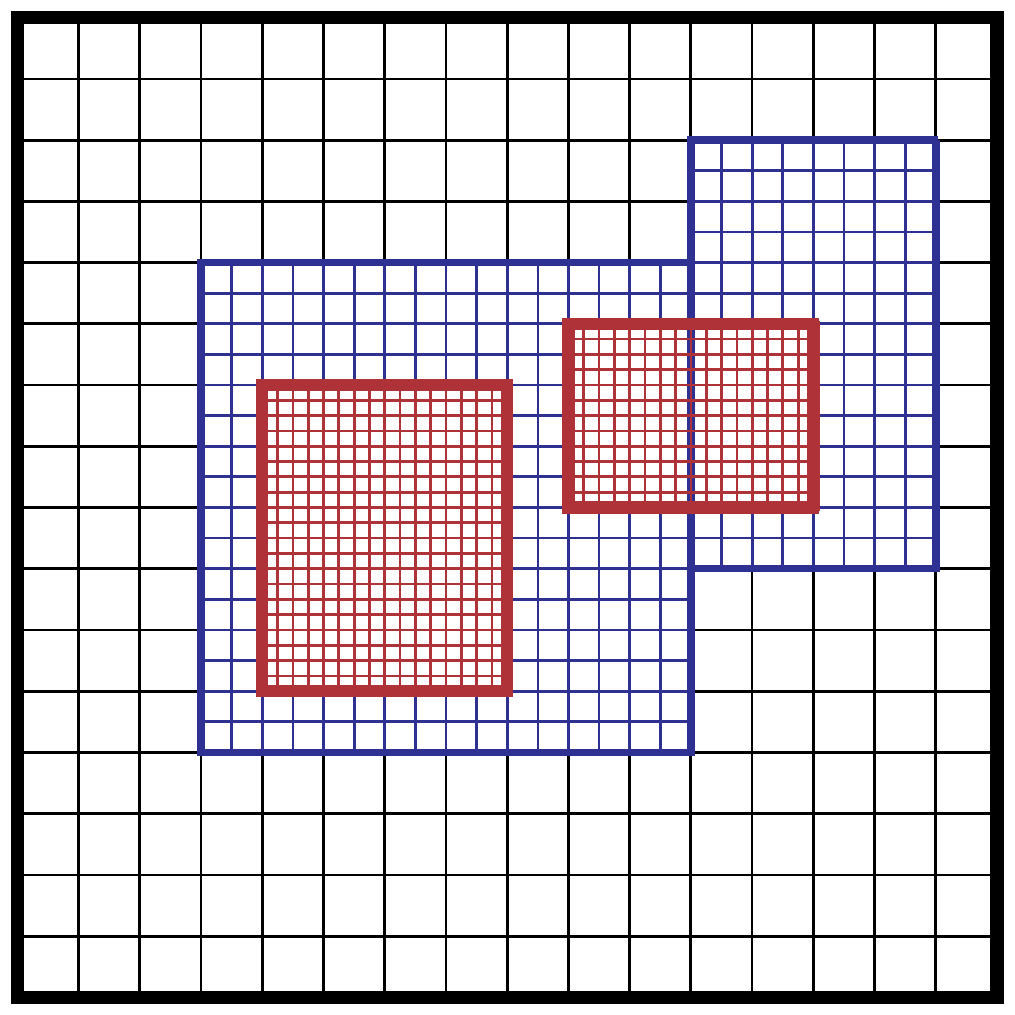
\includegraphics[width=3in]{./Basics/amrgrids.pdf}
  \caption{\label{fig:basics:amrgrids} Example of AMR grids.  There are
    three levels in total.  There are 1, 2 and 2 {\tt Box}es on levels
  0, 1, and 2, respectively.}
\end{figure}

\section{Box, IntVect and IndexType}
\label{sec:basics:box}

{\tt Box} is the data structure for representing a rectangular domain
in indexing space.  For example, in Figure~\ref{fig:basics:amrgrids},
there are 1, 2 and 2 {\tt Box}es on levels 0, 1 and 2, respectively.
{\tt Box} is a dimension dependent class.  It has lower and upper
corners (represented by {\tt IntVect} and an index type (represented
by {\tt IndexType}).  There are no floating-point data in the object.

\subsection{IntVect}

{\idxamrex{IntVect}} is a dimension dependent class representing an
integer vector in {\idxamrex{AMREX\_SPACEDIM}}-dimensional space.  An
{\tt IntVect} can be constructed as follows,
\begin{lstlisting}[language=cpp]
 IntVect iv(AMREX_D_DECL(19, 0, 5));
\end{lstlisting}
Here {\tt AMREX\_D\_DECL} is a macro that expands {\tt
  AMREX\_D\_DECL(19,0,5)} to either {\tt 19} or {\tt 19,0} or {\tt
  19,0,5} depending on the number of dimensions.  The data can be
accessed via {\tt operator[]}, and the internal data pointer can be
returned by function {\tt getVect}.  For example
\begin{lstlisting}[language=cpp]
 for (int idim = 0; idim < AMREX_SPACEDIM; ++idim) {
     amrex::Print() << "iv[" << idim << "] = " << iv[idim] << "\n";
 }
 const int * p = iv.getVect();  // This can be passed to Fortran/C as an array
\end{lstlisting}

The class has a static function {\tt TheZeroVector()} returning the
zero vector, {\tt TheUnitVector()} returning the unit vector, and {\tt
  TheDimensionVector (int dir)} returning a reference to a constant
{\tt IntVect} that is zero except in the {\tt dir}-direction.  Note
the direction is zero-based.  {\tt IntVect} has a number of relational
operators, {\tt ==}, {\tt !=}, {\tt <}, {\tt <=}, {\tt >}, and {\tt
  >=} that can be used for lexicographical comparison (e.g., key of
{\tt std::map}), and a class {\tt IntVect::shift\_hasher} that can be
used as a hash function (e.g., for {\tt std::unordered\_map}).  It
also has various arithmetic operators.  For example,
\begin{lstlisting}[language=cpp]
 IntVect iv(AMREX_D_DECL(19, 0, 5));
 IntVect iv2((AMREX_D_DECL(4, 8, 0));
 iv += iv2;  // iv is now (23,8,5)
 iv *= 2;    // iv is now (46,16,10);
\end{lstlisting}

In AMR codes, one often needs to do refinement and coarsening on {\tt
  IntVect}.  The refinement operation can be done with the
multiplication operation.  However, the coarsening requires care
because of the rounding towards zero behavior of integer division in
Fortran, C and C++.  For example {\tt int i = -1/2} gives {\tt i =
  0}, and what we want is usually {\tt i = -1}.  Thus, one should use
the {\tt coarsen} functions:
\begin{lstlisting}[language=cpp]
  IntVect iv(AMREX_D_DECL(127,127,127));
  IntVect coarsening_ratio(AMREX_D_DECL(2,2,2));
  iv.coarsen(2);                 // Coarsen each component by 2
  iv.coarsen(coarsening_ratio);  // Component-wise coarsening
  const auto& iv2 = amrex::coarsen(iv, 2); // Return an IntVect w/o modifying iv
  IntVect iv3 = amrex::coarsen(iv, coarsening_return); // iv not modified
\end{lstlisting}

Finally, we note that {\tt operator<<} is overloaded for {\tt
  IntVect} and therefore one can call
\begin{lstlisting}[language=cpp]
  amrex::Print() << iv << "\n";
  std::cout << iv << "\n";
\end{lstlisting}

\subsection{IndexType}

This class defines an index as being cell based or node based in
each dimension.  The default constructor defines a cell based type in
all directions.  One can also construct an {\tt IndexType} with an
{\tt IntVect} with zero and one representing cell and node,
respectively.
\begin{lstlisting}[language=cpp]
 // Node in x-direction and cell based in y and z-directions
 // (i.e., x-face of numerical cells)
 IndexType xface(IntVect{AMREX_D_DECL(1,0,0)});
\end{lstlisting}
The class provides various functions including
\begin{lstlisting}[language=cpp]
 // True if the IndexType is cell based in all directions.
 bool cellCentered () const;

 // True if the IndexType is cell based in dir-direction.
 bool cellCentered (int dir) const;

 // True if the IndexType is node based in all directions.
 bool nodeCentered () const;

 // True if the IndexType is node based in dir-direction.
 bool nodeCentered (int dir) const;
\end{lstlisting}

Index type is a very important concept in \amrex.  It is a way of
representing the notion of indices $i$ and $i+1/2$.

\subsection{Box}

A {\tt Box} is an abstraction for defining discrete regions of {\tt
  AMREX\_SPACEDIM}-dimensional indexing space.  {\tt Box}es have an
{\tt IndexType} and two {\tt IntVect}s representing the lower and
upper corners.  Boxes can exist in positive and negative indexing
space.   Typical ways of defining a {\tt Box} are
\begin{lstlisting}[language=cpp]
 IntVect lo(AMREX_D_DECL(64,64,64));
 IntVect hi(AMREX_D_DECL(127,127,127));
 IndexType typ({AMREX_D_DECL(1,1,1)});
 Box cc(lo,hi);        // By default, Box is cell based.
 Box nd(lo,hi+1,typ);  // Construct a nodal Box.
 Print() << "A cell-centered Box " << cc << "\n";
 Print() << "An all nodal Box    " << nd << "\n";
\end{lstlisting}
Depending the dimensionality, the output of the code above is
\begin{verbatim}
  A cell-centered Box ((64,64,64) (127,127,127) (0,0,0))
  An all nodal Box    ((64,64,64) (128,128,128) (1,1,1))
\end{verbatim}
For simplicity, we will assume it is 3D for the rest of this section.
In the output, three integer tuples for each box are the lower corner
indices, upper corner indices, and the index types.  Note that {\tt 0}
and {\tt 1} denote cell and node, respectively.  For each tuple like
{\tt (64,64,64)}, the 3 numbers are for 3 directions.  The two {\tt
  Box}es in the code above represent different indexing views of the
same domain of $64^3$ cells.  Note that in \amrex\ convention, the
lower side of a cell has the same integer value as the cell centered
index.  That is if we consider a cell based index represent $i$, the
nodal index with the same integer value represents $i-1/2$.
Figure~\ref{fig:basics:indextypes} shows a 2D example of various index
types.  

\begin{figure}
  \centering
  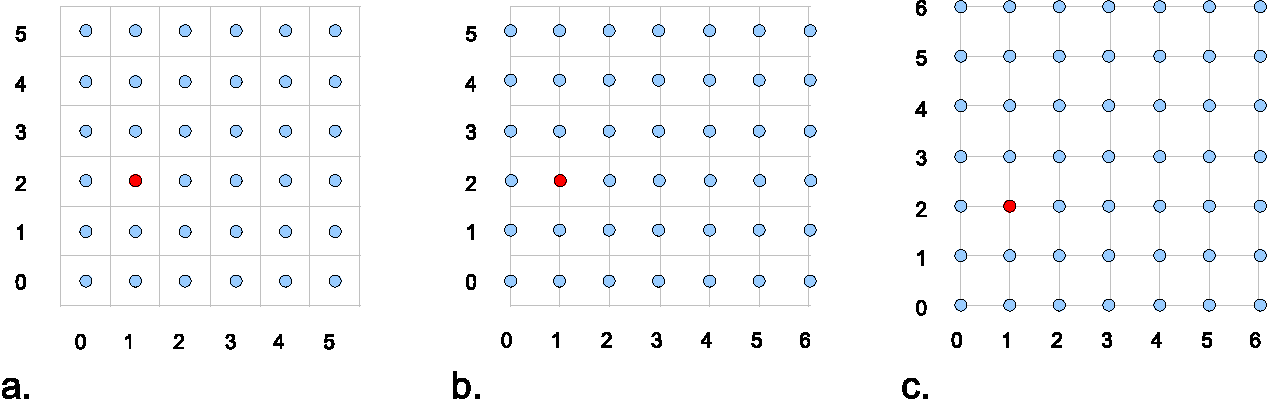
\includegraphics[width=5in]{./Basics/indextypes.pdf}
  \caption{\label{fig:basics:indextypes} Some of the different index
    types in two dimensions: (a) cell-centered, (b) face-centered,
    i.e., nodal in one dimensions ($x$) only, and (c) corner/nodal,
    i.e., nodal in all dimensions.  Note that for data that is nodal
    in one or more direction, the integer index corresponds to the
    lower boundary in that direction.}
\end{figure}

There are a number of ways of converting a {\tt Box} from one type to
another.
\begin{lstlisting}[language=cpp]
  Box b0 ({64,64,64}, {127,127}); // Index type: (cell, cell, cell)

  Box b1 = surroundingNodes(b0);  // A new Box with type (node, node, node)
  Print() << b1;                  // ((64,64,64) (128,128,128) (1,1,1))
  Print() << b0;                  // Still ((64,64,64) (127,127,127) (0,0,0))

  Box b2 = enclosedCells(b1);     // A new Box with type (node, node, node)
  if (b2 == b0) {                 // Yes, they are identical.
     Print() << "b0 and b2 are identical!\n";
  }

  Box b3 = convert(b0, {0,1,0});  // A new Box with type (cell, node, cell)
  Print() << b3;                  // ((64,64,64) (127,128,127) (0,1,0))

  b3.convert({0,0,1});            // Convert b0 to type (cell, cell, node)
  Print() << b3;                  // ((64,64,64) (127,127,128) (0,0,1))

  b3.surroundingNodes();          //  Exercise for you
  b3.enclosedCells();             //  Exercise for you
\end{lstlisting}

The internal data of {\tt Box} can be accessed via various member functions.
Examples are
\begin{lstlisting}[language=cpp]
  const IntVect& smallEnd () const&;  // Get the small end of the Box
  int bigEnd (int dir) const;         // Get the big end in dir direction
  const int* loVect () const&;        // Get a const pointer to the lower end
  const int* hiVect () const&;        // Get a const pointer to the upper end
\end{lstlisting}

{\tt Box}es can be refined and coarsened.  Refinement or coarsening
does not change the index type.  Some examples are shown below.
\begin{lstlisting}[language=cpp]
  Box ccbx ({16,16,16}, {31,31,31});
  ccbx.refine(2);
  Print() << ccbx;                   // ((32,32,32) (63,63,63) (0,0,0))
  Print() << ccbx.coarsen(2);        // ((16,16,16) (31,31,31) (0,0,0))

  Box ndbx ({16,16,16}, {32,32,32}, {1,1,1});
  ndbx.refine(2);
  Print() << ndbx;                   // ((32,32,32) (64,64,64) (1,1,1))
  Print() << ndbx.coarsen(2);        // ((16,16,16) (32,32,32) (1,1,1))

  Box facebx ({16,16,16}, {32,31,31}, {1,0,0});
  facebx.refine(2);
  Print() << facebx;                 // ((32,32,32) (64,63,63) (1,0,0))
  Print() << facebx.coarsen(2);      // ((16,16,16) (32,31,31) (1,0,0))

  Box uncoarsenable ({16,16,16}, {30,30,30});
  print() << uncoarsenable.coarsen(2); // ({8,8,8}, {15,15,15});
  print() << uncoarsenable.refine(2);  // ({16,16,16}, {31,31,31});
                                       // Different from the original!
\end{lstlisting}
Note that refinement and coarsening behaviors depend on the indexing
type.  One should think the refinement and coarsening in AMR context
that refined or coarsened {\tt Box} still covers the same physical
domain.  {\tt Box uncoarsenable} in the example above is considered
uncoarsenable because its coarsened version does not cover the same
physical domain in the AMR context.

{\tt Box}es can grow and they can grow in all directions or just one
direction.  There are a number of {\tt grow} functions.  Some are
member functions of the {\tt Box} class and others are non-member
functions in the {\tt amrex} namespace. 

{\tt Box} class provides the following member functions testing if a {\tt
  Box} or {\tt IntVect} is contained within this {\tt Box}.  Note that
it is a runtime error if the two {\tt Box}es have different types.
\begin{lstlisting}[language=cpp]
  bool contains (const Box& b) const;
  bool strictly_contains (const Box& b) const;
  bool contains (const IntVect& p) const;
  bool strictly_contains (const IntVect& p) const;
\end{lstlisting}

Another very common operation is the intersection of two {\tt Box}es
like in the following examples.
\begin{lstlisting}[language=cpp]
  Box b0 ({16,16,16}, {31,31,31});
  Box b1 ({ 0, 0,30}, {23,23,63});
  if (b0.intersects(b1)) {                  // true
      Print() << "b0 and b1 intersect.\n"; 
  }

  Box b2 = b0 & b1;     // b0 and b1 unchanged
  Print() << b2;        // ((16,16,30) (23,23,31) (0,0,0))

  Box b3 = surroundingNodes(b0) & surroundingNodes(b1); // b0 and b1 unchanged
  Print() << b3;        // ((16,16,30) (24,24,32) (1,1,1))

  b0 &= b2;             // b2 unchanged
  Print() << b0;        // ((16,16,30) (23,23,31) (0,0,0))

  b0 &= b3;             // Runtime error because of type mismatch!
\end{lstlisting}

\section{RealBox and Geometry}

A {\tt RealBox} stores the physical location in floating-point numbers
of the lower and upper corners of a rectangular domain.

{\tt Geometry} class describes problem domain and coordinate system
for rectangular problem domains.  A {\tt Geometry} object can be
constructed with
\begin{lstlisting}[language=cpp]
  explicit Geometry (const Box&     dom,
                     const RealBox* rb     = nullptr,
                     int            coord  = -1,
                     int*           is_per = nullptr);
\end{lstlisting}
Here the constructor takes a {\tt Box} specifying the indexing space
domain, an optional argument of {\tt RealBox} pointer specifying the
physical domain, an optional {\tt int} specifying coordinate system
type, and an optional {\tt int *} specifying periodicity.  If a {\tt
  RealBox} is not given, \amrex\ will construct one based on {\tt
  ParmParse} parameters, {\tt geometry.prob\_lo} and {\tt
  geometry.prob\_hi}, where each of the parameter is an array of {\tt
  AMREX\_SPACEDIM} real numbers.  It's a runtime error if this fails.
The optional argument for coordinate system is an integer type with
valid values being 0 (Cartesian), or 1 (cylindrical), or 2
(spherical).  If it is invalid as in the case of the default argument
value, \amrex\ will query the {\tt ParmParse} database for {\tt
  geometry.coord\_sys} and use it if one is found.  If it cannot find
the parameter, the coordinate system is set to 0 (i.e., Cartesian
coordinates).  {\tt Geometry} class has the concept of periodicity.
An optional argument can be passed specifying periodicity in each
dimension.  If it is not given, the domain is assumed to be
non-periodic unless there is the {\tt ParmParse} integer array
parameter {\tt geometry.is\_periodic} with {\tt 0} denoting
non-periodic and {\tt 1} denoting periodic.  Below is an example of
defining a {\tt Geometry} for a periodic rectangular domain of
$[-1.0,1.0]$ in each direction discretized with $64$ numerical cells
in each direction.
\begin{lstlisting}[language=cpp]
  int n_cell = 64;

  // This defines a Box with n_cell cells in each direction.
  Box domain(IntVect{AMREX_D_DECL(       0,        0,        0)},
             IntVect{AMREX_D_DECL(n_cell-1, n_cell-1, n_cell-1)});

  // This defines the physical box, [-1,1] in each direction.
  RealBox real_box({AMREX_D_DECL(-1.0,-1.0,-1.0)},
                   {AMREX_D_DECL( 1.0, 1.0, 1.0)});
  
  // This says we are using Cartesian coordinates
  int coord = 0;
  
  // This sets the boundary conditions to be doubly or triply periodic
  std::array<int,AMREX_SPACEDIM> is_periodic {AMREX_D_DECL(1,1,1)};
  
  // This defines a Geometry object
  Geometry geom(domain, &real_box, coord, is_periodic.data());
\end{lstlisting}

A {\tt Geometry} object can return various information of the physical
domain and the indexing space domain.  For example,
\begin{lstlisting}[language=cpp]
  const Real* problo = geom.ProbLo();  // Lower corner of the physical domain
  Real yhi = geom.ProbHi(1);           // y-direction upper corner
  const Real* dx = geom.CellSize();    // Cell size for each direction
  const Box& domain = geom.Domain();   // Index domain
  bool is_per = geom.isPeriodic(0);    // Is periodic in x-direction?
\end{lstlisting}


\section{BoxArray}
\label{sec:basics:ba}

{\tt BoxArray} is a class for storing a collection of {\tt Box}es on
a single AMR level.  One can make a {\tt BoxArray} out of a single {\tt Box}
and then chop it into multiple {\tt Box}es.
\begin{lstlisting}[language=cpp]
  Box domain(IntVect{0,0,0}, IntVect{127,127,127});
  BoxArray ba(domain);  // Make a new BoxArray out of a single Box
  Print() << "BoxArray size is " << ba.size() << "\n";  // 1
  ba.maxSize(64);       // Chop into boxes of 64^3 cells
  Print() << ba;
\end{lstlisting}
The output is like below,
\begin{verbatim}
  (BoxArray maxbox(8)
         m_ref->m_hash_sig(0)
  ((0,0,0) (63,63,63) (0,0,0)) ((64,0,0) (127,63,63) (0,0,0))
  ((0,64,0) (63,127,63) (0,0,0)) ((64,64,0) (127,127,63) (0,0,0))
  ((0,0,64) (63,63,127) (0,0,0)) ((64,0,64) (127,63,127) (0,0,0))
  ((0,64,64) (63,127,127) (0,0,0)) ((64,64,64) (127,127,127) (0,0,0)) )
\end{verbatim}
It shows that {\tt ba} now has 8 {\tt Box}es, and it also prints out
each {\tt Box}es.  

In \amrex, {\tt BoxArray} is a global data structure.  It holds all
the {\tt Box}es in a collection, even though a single process in a
parallel run only owns some of the {\tt Box}es via domain
decomposition.  In the example above, a 4-process run may divide the
work and each process owns say 2 {\tt Box}es
(Section~\ref{sec:basics:dm}).  Each process can then allocate memory
for the floating point data on the {\tt Box}es it owns
(Sections~\ref{sec:basics:multifab} \& \ref{sec:basics:fab}). 

{\tt BoxArray} has an indexing type, just like {\tt Box}.  Each {\tt
  Box} in a {\tt BoxArray} has the same type as the {\tt BoxArray}
itself.  In the following example, we show how one can convert {\tt
  BoxArray} to a different type. 
\begin{lstlisting}[language=cpp]
  BoxArray cellba(Box(IntVect{0,0,0}, IntVect{63,127,127}));
  cellba.maxSize(64);
  BoxArray faceba = cellba;
  // convert to index type (cell, cell, node)
  faceba.convert(IntVect{0,0,1});
  // Return an all node BoxArray
  const BoxArray& nodeba = amrex::convert(faceba, IntVect{1,1,1});
  Print() << cellba[0] << "\n";  // ((0,0,0) (63,63,63) (0,0,0))
  Print() << faceba[0] << "\n";  // ((0,0,0) (63,63,64) (0,0,1))  
  Print() << nodeba[0] << "\n";  // ((0,0,0) (64,64,64) (1,1,1))
\end{lstlisting}

As shown in the example above, {\tt BoxArray} has an {\tt operator[]}
that returns a {\tt Box} given an index.  It should be emphasized that
there is a difference between its behavior and the usual behavior of
an subscript operator one might expect.  The subscript operator in
{\tt BoxArray} returns by value instead of reference.  This means code
like below is meaningless because it modifies a temporary return
value. 
\begin{lstlisting}[language=cpp]
  ba[3].coarsen(2);  // DO NOT DO THIS!  Doesn't do what one might expect.
\end{lstlisting}

{\tt BoxArray} has a number of member functions that allow the {\tt
  Box}es to be modified.  For example,
\begin{lstlisting}[language=cpp]
  BoxArray& refine (int refinement_ratio);   // Refine each Box in BoxArray
  BoxArray& refine (const IntVect& refinement_ratio);
  BoxArray& coarsen (int refinement_ratio);  // Coarsen each Box in BoxArray
  BoxArray& coarsen (const IntVect& refinement_ratio);
\end{lstlisting}

We have mentioned at the beginning of this section that {\tt BoxArray}
is a global data structure storing {\tt Box}es owned by all processes.
The operation of deep copy is thus undesirable because the operation
itself is expensive and the extra copy wastes memory.  The
implementation of the {\tt BoxArray} class uses {\tt std::shared\_ptr}
to an internal container holding the actual {\tt Box} data.  Thus
making a copy of {\tt BoxArray} is a quite cheap operation.  The
conversion of types and coarsening are also cheap because they can
share the internal data with the original {\tt BoxArray}.  Function
{\tt refine} does create a new deep copy of the original data.  Also
note that a {\tt BoxArray} and its variant with a different type share
the same internal data is an implementation detail.  We discuss this
so that the users are aware of the performance and resource cost.
Conceptually we can think of them as completely independent of each
other.

For advanced users, \amrex\ provides functions performing the
intersection of a {\tt BoxArray} and a {\tt Box}.  These functions are
much faster than a naive implementation of performing intersection of
the {\tt Box} with each {\tt Box} in the {\tt BoxArray}.  If one needs
to perform those intersections, functions {\tt amrex::intersect}, {\tt
  BoxArray:: intersects} and {\tt BoxArray::intersections} should be
used.

\section{DistributionMapping}
\label{sec:basics:dm}

{\tt DistributionMapping} is a class describes which process owns the
data living on the domains specified by the {\tt Box}es in a {\tt
  BoxArray}.  Like {\tt BoxArray}, {\tt DistributionMapping} has an
element for each {\tt Box}, including the ones owned by other parallel
processes.  A way to construct a {\tt DistributionMapping} object
given a {\tt BoxArray} is as follows.
\begin{lstlisting}[language=cpp]
  DistributionMapping dm {ba};
\end{lstlisting}
Oftentimes what one needs is simply making a copy. 
\begin{lstlisting}[language=cpp]
  DistributionMapping dm {another_dm};
\end{lstlisting}
Note that this class is built using {\tt std::shared\_ptr}.  Thus
making a copy is relatively cheap in terms of performance and memory
resources.  This class has a subscript operator that returns the
process ID at a given index.

By default, {\tt DistributionMapping} uses an algorithm based on space
filling curve to determine distribution.  One can change the default
via {\tt ParmParse} paramter {\tt DistributionMapping.strategy}.  {\tt
  KNAPSACK} is a common choice that is optimized for load balance.
One can also explicitly construct a certain type of distribution.
{\tt DistributionMapping} class allows the user to have complete control by
passing an array of integers. 
\begin{lstlisting}[language=cpp]
  DistributionMapping dm;   // empty object
  Array<int> pmap;
  // The user fills the pmap array with the values specifying owner processes
  dm.define(pmap);  // Build DistributionMapping given an array of process IDs.
\end{lstlisting}


\section{BaseFab, FArrayBox and IArrayBox}
\label{sec:basics:fab}

\amrex\ is a block-structured AMR framework.  Although AMR introduces
irregularity to the data and algorithms, there is regularity at the
block/{\tt Box} level due to rectangular domain and the data structure
at the {\tt Box} level is conceptually simple.  {\tt BaseFab} is a
class template for multi-dimensional array-like data structure on a
{\tt Box}.  The template parameter is typically basic types such as
{\tt Real}, {\tt int} or {\tt char}.  The dimensionality of the array
is {\tt AMREX\_SPACEDIM} plus one.  The additional dimensional is for
the number of components.  The data are internally stored in a
contiguous block of memory in Fortran array order (i.e., column-major
order) for $(x,y,z,\mathrm{component})$, and each component also
occupies a contiguous block of memory because of the ordering.  For
example, a {\tt BaseFab<Real>} with 4 components defined on a
three-dimensional {\tt Box(IntVect\{-4,8,32\},IntVect\{32,64,48\})} is
like a Fortran array of {\tt real(amrex\_real),
  dimension(-4:32,8:64,32:48,0:3)}.  Note that the convention in \cpp\
part of \amrex\ is the component index is zero based.  The code for
constructing such an object is as follows,
\begin{lstlisting}[language=cpp]
  Box bx(IntVect{-4,8,32}, IntVect{32,64,48});
  int numcomps = 4;
  BaseFab<Real> fab(bx,numcomps);
\end{lstlisting}

Most applications do not use {\tt BaseFab} directly, but utilize
specialized classes derived from {\tt BaseFab}.  The most common types
are {\tt FArrayBox} derived from {\tt BaseFab<Real>} and {\tt
  IArrayBox} derived from {\tt BaseFab<int>}.

These derived classes also obtain many {\tt BaseFab} member functions
via inheritance.  We now show some common usages of these functions.
To get the {\tt Box} where a {\tt BaseFab} or its derived object is
defined, one can call
\begin{lstlisting}[language=cpp]
  const Box& box() const;
\end{lstlisting}
To the number of component, one can call
\begin{lstlisting}[language=cpp]
  int nComp() const;
\end{lstlisting}
To get a pointer to the array data, one can call
\begin{lstlisting}[language=cpp]
  T* dataPtr(int n=0);     // Data pointer to the nth component
                           // T is template parameter (e.g., Real)
  const T* dataPtr(int n=0) const; // const version
\end{lstlisting}
The typical usage of the returned pointer is then to pass it to a
Fortran or C function that works on the array data (see
Section~\ref{sec:basics:fortran}).
{\tt BaseFab} has several functions that set the array data to a
constant value (e.g., 0).  Two examples are as follows.  
\begin{lstlisting}[language=cpp]
  void setVal(T x);        // Set all data to x
  // Set the sub-region specified by bx to value x starting from component
  // nstart.  ncomp is the total number of component to be set.
  void setVal(T x, const Box& bx, int nstart, int ncomp);
\end{lstlisting}
One can copy data from one {\tt BaseFab} to another.
\begin{lstlisting}[language=cpp]
  BaseFab<T>& copy (const BaseFab<T>& src, const Box& srcbox, int srccomp,
                    const Box& destbox, int destcomp, int numcomp);
\end{lstlisting}
Here the function copies the data from the region specified by {\tt
  srcbox} in the source {\tt BaseFab src} into the region specified by
{\tt destbox} in the destination {\tt BaseFab} that invokes the
function.  Note that although {\tt srcbox} and {\tt destbox} may be
different, they must be the same size and shape, otherwise a runtime
error occurs.  The user also specifies how many components ({\tt int
  numcomp}) are copied starting at component {\tt srccomp} in {\tt
  src} and stored starting at component {\tt destcomp}.  {\tt BaseFab}
has functions returning the minimum or maximum value.
\begin{lstlisting}[language=cpp] 
  T min (int comp=0) const;  // Minimum value of given component.
  T min (const Box& subbox, int comp=0) const; // Minimum value of given 
                                               // component in given subbox.
  T max (int comp=0) const;  // Maximum value of given component.
  T max (const Box& subbox, int comp=0) const; // Maximum value of given 
                                               // component in given subbox.
\end{lstlisting}

{\tt BaseFab} also has many arithmetic functions.  Here are some
examples using {\tt FArrayBox}.
\begin{lstlisting}[language=cpp]
  Box box(IntVect{0,0,0}, IntVect{63,63,63});
  int ncomp = 2;
  FArrayBox fab1(box, ncomp);
  FArrayBox fab2(box, ncomp);
  fab1.setVal(1.0);    // Fill fab1 with 1.0
  fab1.mult(10.0, 0);  // Multiply component 0 by 10.0
  fab2.setVal(2.0);    // Fill fab2 with 2.0
  Real a = 3.0;
  fab2.saxpy(a, fab1); // For both components, fab2 <- a * fab1 + fab2
\end{lstlisting}
For more complicated expressions that not supported, one can write
Fortran or C functions for those (Section~\ref{sec:basics:fortran}).
Note that {\tt BaseFab} does provide operators for accessing the
data directly in \cpp.  For example, the {\tt saxpy} example above can
be done with
\begin{lstlisting}[language=cpp]
  // Iterate over all components
  for (int icomp=0; icomp < fab1.nComp(); ++icomp) {
      // Iterate over all cells in Box
      for (BoxIterator bit(fab1.box()); bit.ok(); ++bit) {
          // bit() returns IntVect
          fab2(bit(),icomp) = a * fab1(bit(),icomp) + fab2(bit(),icomp);
      }
  }
\end{lstlisting}
But this approach is generally not recommended for performance reason.
However, it can be handy for debugging.

{\tt BaseFab} and its derived classes are containers data on {\tt
  Box}.  We recall that {\tt Box} has types
(Section~\ref{sec:basics:box}).  The examples in this section so far
use the default cell based type.  However, some functions will result
in a runtime error if the types mismatch.  For example.
\begin{lstlisting}[language=cpp]
  Box ccbx ({16,16,16}, {31,31,31});           // cell centered box
  Box ndbx ({16,16,16}, {31,31,31}, {1,1,1});  // nodal box
  FArrayBox ccfab(ccbx);
  FArrayBox ndfab(ndbx);
  ccfab.setVal(0.0);
  ndfab.copy(ccfab);   // runtime error due to type mismatch
\end{lstlisting}

Because it typically contains a lot of data, {\tt BaseFab}'s copy
constructor and copy assignment operator are disabled for performance
reason.  However, it does provide a move constructor.  In addition, it
also provides a constructor for making an alias of an existing
object.  Here is an example using {\tt FArrayBox}.
\begin{lstlisting}[language=cpp]
  FArrayBox orig_fab(box, 4);  // 4-component FArrayBox
  // Make a 2-component FArrayBox that is an alias of rhs
  // starting from component 1.
  FArrayBox alias_fab(rhs, amrex::make_alias, 1, 2);
\end{lstlisting}
In the example, the alias {\tt FArrayBox} has only two components even
though the original one has four components.  The alias has a sliced
component view of the original {\tt FArrayBox}.  This is possible
because of the array ordering.  It is however not possible to slice in
the real space (i.e., the first {\tt AMREX\_SPACEDIM} dimensions).
Note that no new memory is allocated in constructing the alias and the
alias contains a non-owning pointer.  It should be emphasized that the
alias will contain a dangling pointer after the original {\tt
  FArrayBox} reaches its end of life.

\section{FabArray, MultiFab and iMultiFab}
\label{sec:basics:multifab}

{\tt FabArray<FAB>} is a class template for a collection of {\tt FAB}s
on the same AMR level associated with a {\tt BoxArray}
(Section~\ref{sec:basics:ba}).  The template parameter {\tt FAB} is
usually {\tt BaseFab<T>} or its derived classes (e.g., {\tt
  FArrayBox}).  However, it can also be used to hold other data
structures.  To construct a {\tt FabArray}, a {\tt BoxArray} must be
provided because it is intended to hold {\emph{grid}} data defined on
a union of rectangular regions embedded in a uniform index space.  For
example, an {\tt FabArray} object can be used to hold data for one
level of the example grids of Figure~\ref{fig:basics:amrgrids}.  The
{\tt BoxArray} on level 2 ({\emph{red}) has two {\tt Box}es.

{\tt FabArray} is a parallel data structure that the data (i.e.,
{\tt FAB}) are distributed among parallel processes.  On each process,
the {\tt FabArray} contains only the {\tt FAB} objects owned by this
process, and the process operates only on its local data.  For
operations that require data owned by other processes, remote
communications are involved.  Thus, the construction of a {\tt
  FabArray} requires a {\tt DistributionMapping}
(Section~\ref{sec:basics:dm}) that specifies which process owns which
{\tt Box}.  For level 2 ({\emph{red}) in
Figure~\ref{fig:basics:amrgrids}, there are two {\tt Box}es.  Suppose
there are two parallel processes, and we use a {\tt
  DistributionMapping} that assigns one {\tt Box} to each process.
For {\tt FabArray} on each process, it is built on a {\tt BoxArray} with
2 {\tt Box}es, but contains only one {\tt FAB}.  

In \amrex, there are some specialized classes derived from {\tt
  FabArray}.  The {\tt iMultiFab} class is derived from {\tt
  FabArray<IArrayBox>}.  The most commonly used {\tt FabArray} kind
class is {\tt MultiFab} derived from {\tt FabArray<FArrayBox>}.  In
the rest of this section, we use {\tt MultiFab} as example.  However,
these concepts are equally applicable to other types of {\tt
  FabArray}s.  There are many ways to define a {\tt MultiFab}.  For
example,
\begin{lstlisting}[language=cpp]
  // ba is BoxArray
  // dm is DistributionMapping
  int ncomp = 4;
  int ngrow = 1;
  MultiFab mf(ba, mf, ncomp, ngrow);
\end{lstlisting}
Here we define a {\tt MultiFab} with 4 components and 1 ghost cell.  A
{\tt MultiFab} contains a number of {\tt FArrayBox}es
(Section~\ref{sec:basics:fab}) defined on {\tt Box}es grown by the
number of ghost cells (1 in this example).  That is the {\tt Box} in
the {\tt FArrayBox} is not exactly the same as in the {\tt BoxArray}.
If the {\tt BoxArray} has a {\tt Box\{(8,8,8) (15,15,15)\}}, the one
used for constructing {\tt FArrayBox} will be {\tt Box\{(7,7,7)
  (16,16,16)\}} in this example.  For cells in {\tt FArrayBox}, we
call those in the original {\tt Box} valid cells and the grown part
ghost cells.  Note that {\tt FArrayBox} itself alone does not have the
concept of ghost cell, whereas ghost cell is a key concept of {\tt
  MultiFab} that allows for local operations on ghost cell data
originated from remote processes.  We will discuss how to fill ghost
cells with data from valid cells later in this section.  {\tt
  MultiFab} also has a default constructor.  One can define an empty
{\tt MultiFab} first and then call the {\tt define} function as
follows.
\begin{lstlisting}[language=cpp]
  MultiFab mf;
  // ba is BoxArray
  // dm is DistributionMapping
  int ncomp = 4;
  int ngrow = 1;
  mf.define(ba, mf, ncomp, ngrow);
\end{lstlisting}
Given an existing {\tt MultiFab}, one can also make an alias {\tt
  MultiFab} as follows.
\begin{lstlisting}[language=cpp]
  // orig_mf is an existing Multifab
  int start_comp = 3;
  int num_comps = 1;
  MultiFab alias_mf(orig_mf, amrex::make_alias, start_comp, num_comps);
\end{lstlisting}
Here the first integer parameter is the starting component in the
original {\tt MultiFab} that will become component 0 in the alias {\tt
  MultiFab} and the second integer parameter is the number of
components in the alias.  It's a runtime error if the sum of the two
integer parameters is greater than the number of the components in the
original {\tt MultiFab}.  Note that the alias {\tt MultiFab} has
exactly the same number of ghost cells as the original {\tt MultiFab}.

We often need to build new {\tt MultiFab}s that have the same {\tt
  BoxArray} and {\tt DistributionMapping} as a given {\tt MultiFab}.
Below is an example of how to achieve this.
\begin{lstlisting}[language=cpp]
  // mf0 is an already defined MultiFab
  const BoxArray& ba = mf0.boxArray();
  const DistributionMapping& dm = mf0.DistributionMap();
  int ncomp = mf0.nComp();
  int ngrow = mf0.ngrow();
  MultiFab mf1(ba,dm,ncomp,ngrow);  // new MF with the same ncomp and ngrow
  MultiFab mf2(ba,dm,ncomp,0);      // new MF with no ghost cells
  // new MF with 1 component and 2 ghost cells
  MultiFab mf3(mf0.boxArray(), mf0.DistributionMap(), 1, 2);               
\end{lstlisting}

As we have repeatedly mentioned in this chapter that {\tt Box} and
{\tt BoxArray} have various index types.  Thus, {\tt MultiFab} also
has an index type that is obtained from the {\tt BoxArray} used for
defining the {\tt MultiFab}.  It should be noted again that index type
is a very important concept in \amrex.  Let's consider an example of a
finite-volume code, in which the state is defined as cell averaged
variables and the fluxes are defined as face averaged variables.
\begin{lstlisting}[language=cpp]
  // ba is cell-centered BoxArray
  // dm is DistributionMap
  int ncomp = 3;  // Suppose the system has 3 components
  int ngrow = 0;  // no ghost cells
  MultiFab state(ba, dm, ncomp, ngrow);
  MultiFab xflux(amrex::convert(ba, IntVect{1,0,0}), dm, ncomp, 0);
  MultiFab yflux(amrex::convert(ba, IntVect{0,1,0}), dm, ncomp, 0);
  MultiFab zflux(amrex::convert(ba, IntVect{0,0,1}), dm, ncomp, 0);
\end{lstlisting}
Here all {\tt MultiFab} use the same {\tt DistributionMapping}, but
their {\tt BoxArray}s have different.  The state is cell based,
whereas the fluxes are on the faces.  Suppose the cell based {\tt
  BoxArray} contains a {\tt Box\{(8,8,16), (15,15,31)\}}.  The state
on that {\tt Box} is conceptually a Fortran Array with the dimension
of {\tt (8:15,8:15,16:31,0:2)}.  The fluxes are arrays with slightly
different indices.  For example, the $x$-direction flux for that {\tt
  Box} has the dimension of {\tt (8:16,8:15,16:31,0:2)}.  Note there is
an extra element in $x$-direction.  

The {\tt MultiFab} provides many functions performing common
arithmetic operations on a {\tt MultiFab} or between {\tt MultiFab}s
built with the {\emph{same}} {\tt BoxArray} and {\tt DistributionMap}.
For example,
\begin{lstlisting}[language=cpp]
  Real dmin = mf.min(3);   // Minimum value in component 3 of MultiFab mf
                           // no ghost cells included
  Real dmax = mf.max(3,1); // Maximum value in component 3 of MultiFab mf
                           // including 1 ghost cell
  mf.setVal(0.0);          // Set all values to zero including ghost cells

  MultiFab::Add(mfdst, mfsrc, sc, dc, nc, ng);  // Add mfsrc to mfdst
  MultiFab::Copy(mfdst, mfsrc, sc, dc, nc, ng); // Copy from mfsrc to mfdst
  // MultiFab mfdst: destination 
  // MultiFab mfsrc: source
  // int      sc   : starting component index in mfsrc for this operation
  // int      dc   : starting component index in mfdst for this operation
  // int      sc   : number of components for this operation
  // int      ng   : number of ghost cells involved in this operation
\end{lstlisting}
We refer the reader to {\tt Src/Base/AMReX\_MultiFab.H} and {\tt
  Src/Base/AMReX\_FabArray.H} for more details.  It should be noted
again it is a runtime error if the two {\tt MultiFab}s passed to functions
like {\tt MultiFab::Copy} are not built with the {\emph{same}} {\tt
  BoxArray} (including index type) and {\tt DistributionMap}. 

It is usually the case that the {\tt Box}es in the {\tt BoxArray} used
for building a {\tt MultiFab} are non-intersecting except that they
can be overlapping due to nodal index type.  However, {\tt MultiFab}
can have ghost cells, and in that case {\tt FArrayBox}es are defined
on {\tt Box}es larger than the {\tt Box}es in the {\tt BoxArray}.
Parallel communication is then needed to fill the ghost cells with
valid cell data from other {\tt FArrayBox}es possibly on other
parallel processes.  The function for performing this type of
communication is {\tt FillBoundary}.
\begin{lstlisting}[language=cpp]
  MultiFab mf(...parameters omitted...);
  Geometry geom(...parameters omitted...);
  mf.FillBoundary();                    // Fill ghost cells for all components
                                        // Periodic boundaries are not filled.
  mf.FillBoundary(geom.periodicity());  // Fill ghost cells for all components
                                        // Periodic boundaries are filled.
  mf.FillBoundary(2, 3);        // Fill 3 components starting from component 2
  mf.FillBoundary(geom.periodicity(), 2, 3);
\end{lstlisting}
Note that {\tt FillBoundary} does not modify any valid cells.  Also
note that {\tt MultiFab} itself does not have the concept of
periodicity boundary, but {\tt Geometry} has, and we can provide that
information so that periodic boundaries can be filled as well.  You
might have noticed that a ghost cell could overlap with multiple valid
cells from different {\tt FArrayBox}es in the case of nodal index
type.  In that case, it is unspecified that which valid cell's value
is used to fill the ghost cell.  It ought to be the case the values in
those overlapping valid cells are the same.

Another type of parallel communication is copying data from one {\tt
  MultiFab} to another {\tt MultiFab} with a different {\tt BoxArray}
or the same {\tt BoxArray} with a different {\tt
  DistributionMapping}.   The data copy is performed on the regions of
intersection.  The most generic interface for this is
\begin{lstlisting}[language=cpp]
  mfdst.ParallelCopy(mfsrc, sc, dc, nc, sng, snd, period, op);
\end{lstlisting}
Here {\tt mfdst} and {\tt mfsrc} are destination and source {\tt
  MultiFab}s, respectively.  Parameters {\tt sc}, {\tt dc}, and {\tt
  nc} are integers specifying the range of components.  The copy is
performed on {\tt nc} components starting from component {\tt sc} of
{\tt mfsrc} and component {\tt dc} of {\tt mfdst}.  Parameters {\tt
  sng} and {\tt snd} specify the number of ghost cells involved for
the source and destination, respectively.  Parameter {\tt period} is
optional, and by default no periodic copy is performed.  Like {\tt
  FillBoundary}, one can use {\tt Geometry::periodicity()} to provide
the periodicity information.  The last parameter is also optional and
is set to {\tt FabArrayBase::COPY} by default.  One could also use
{\tt FabArrayBase::ADD}.  This determines whether the function copies
or adds data from the source to the destination.  Same as {\tt
  FillBoundary}, if a destination cell has multiple cells as source,
it is unspecified that which source cell is used.  This function has
two variants, in which the periodicity and operation type are also
optional.
\begin{lstlisting}[language=cpp]
  mfdst.ParallelCopy(mfsrc, period, op);  // mfdst and mfsrc must have the same
                                          // number of components
  mfdst.ParallelCopy(mfsrc, sc, dc, nc, period, op);
\end{lstlisting}
Here the number of ghost cells involved is zero if unspecified, and
the copy is performed on all components (assuming the two {\tt
  MultiFab}s have the same number of components).  Similar to {\tt
  FillBoundary}, a destination cell may have multiple sources and
which source is used is unspecified.  

\section{MFIter and Tiling}
\label{sec:basics:mfiter}

In this section, we will first show how {\tt MFIter} works without
tiling.  Then we will introduce the concept of logical tiling.
Finally we will show how logical tiling can be launched via {\tt
  MFIter}. 

\subsection{MFIter without Tiling}
\label{sec:basics:mfiter:notiling}

In Section~\ref{sec:basics:multifab}, we have shown some of the
arithmetic functionalities of {\tt MultiFab}, such as adding two {\tt
  MultiFab}s together.  In this section, we will show how you can
operate on the {\tt MultiFab} data with your own functions.  \amrex\
provides an iterator, {\tt MFIter} for looping over the {\tt
  FArrayBox}es in a {\tt MultiFab}.  For example,
\begin{lstlisting}[language=cpp]
  for (MFIter mfi(mf); mfi.isValid(); ++mfi) // Loop over grids
  {
      // This is the valid Box of the current FArrayBox.
      // By "valid", we mean the original ungrown Box in BoxArray.
      const Box& box = mfi.validbox();

      // A reference to the current FArrayBox in this loop iteration.
      FArrayBox& fab = mf[mfi];

      // Pointer to the floating point data of this FArrayBox.
      Real* a = fab.dataPtr();

      // This is the Box on which the FArrayBox is defined.
      // Note that "abox" includes ghost cells (if there are any),
      // and is thus larger than or equal to "box".
      const Box& abox = fab.box();

      // We can now pass the information to a function that does
      // work on the region specified by box of the data pointed
      // by Real* a.  The data should be viewed as a multidimensional
      // with bounds specified by abox.
      // Function f1 has the signature of
      // void f1(const int*, const int*, Real*, const int*, const int*);
      f1(box.loVect(), box.hiVect(), a, abox.loVect(), abox.hiVect());
  }
\end{lstlisting}
Here function {\tt f1} is usually a Fortran subroutine with ISO C
binding interface like below,
\begin{lstlisting}[language=fortran]
  subroutine f1(lo, hi, a, alo, ahi) bind(c)
    use amrex_fort_module, only : amrex_real
    integer, intent(in) :: lo(3), hi(3), alo(3), ahi(3)
    real(amrex_real),intent(inout)::a(alo(1):ahi(1),alo(2):ahi(2),alo(3):ahi(3))
    integer :: i,j,k
    do     k = lo(3), hi(3)
      do   j = lo(2), hi(2)
        do i = lo(1), hi(1)
          a(i,j,k) = ...
        end do
      end do
    end do
  end subroutine f1
\end{lstlisting}
Here {\tt amrex\_fort\_module} is a Fortran module in \amrex\ and {\tt
  amrex\_real} is a Fortran kind parameter that matches {\tt
  amrex::Real} in \cpp.  In this example, we assume the spatial
dimension is 3.  In 2D, the function interface is different.  In
Section~\ref{sec:basics:fortran}, we will present a dimension agnostic
approach using macros provided by \amrex.

{\tt MFIter} only loops over grids owned by the processes.  For
example, suppose there are 5 {\tt Box}es in total and processes 0 and
1 owns 2 and 3 {\tt Box}es, respectively.  That is the {\tt MultiFab}
on process 0 has 2 {\tt FArrayBox}es, whereas there are 3 {\tt
  FArrayBox}es on process 1.  Thus the numbers of iterations of {\tt
  MFIter} are 2 and 3 on processes 0 and 1, respectively.

In the example above, {\tt MultiFab} is assumed to have a single
component.  If it has multiple component, we can call {\tt int nc =
  mf.nComp()} to get the number of components and pass it to the
kernel function.  There is only one {\tt MultiFab} in the example
above.  Below is an example of working with multiple {\tt MultiFab}s.
Note that these two {\tt MultiFab}s are not necessarily built on the
same {\tt BoxArray}.  But they must have the same {\tt
  DistributionMapping}, and their {\tt BoxArray}s are typically
related (e.g., they are different due to index types).
\begin{lstlisting}[language=cpp]
  // U and F are MultiFabs
  int ncU = U.nComp();   # number of components
  int ncF = F.nComp();
  for (MFIter mfi(F); mfi.isValid(); ++mfi) // Loop over grids
  {
      const Box& box = mfi.validbox();

      const FArrayBox& ufab = U[mfi];
      FArrayBox&       ffab = F[mfi];

      Real* up = ufab.dataPtr();
      Real* fp = ufab.dataPtr();

      const Box& ubox = ufab.box();
      const Box& fbox = ffab.box();

      // Function f2 has the signature of 
      // void f2(const int*, const int*,
      //         const Real*, const int*, const int*, const int*
      //               Real*, const int*, const int*, const int*);
      // This will compute f using u as inputs.
      f2(box.loVect(), box.hiVect(),
         up, ubox.loVect(), ubox.hiVect(), &ncU,
         fp, fbox.loVect(), fbox.hiVect(), &ncF);
  }
\end{lstlisting}
Here again function {\tt f2} is usually a Fortran subroutine with ISO
C binding interface like below,
\begin{lstlisting}[language=fortran]
subroutine f1(lo, hi, u, ulo, uhi, nu, f, flo, fhi, nf) bind(c)
  use amrex_fort_module, only : amrex_real
  integer, intent(in) :: lo(3),hi(3),ulo(3),uhi(3),nu,flo(3),fhi(3),nf
  real(amrex_real),intent(in   )::u(ulo(1):uhi(1),ulo(2):uhi(2),ulo(3):uhi(3),nu)
  real(amrex_real),intent(inout)::f(flo(1):fhi(1),flo(2):fhi(2),flo(3):fhi(3),nf)
  integer :: i,j,k
  do n = 1, nf
    do     k = lo(3), hi(3)
      do   j = lo(2), hi(2)
        do i = lo(1), hi(1)
          f(i,j,k,n) = ... u(...) ...
        end do
      end do
    end do
  end do
end subroutine f1
\end{lstlisting}

\subsection{MFIter with Tiling}
\label{sec:basics:mfiter:tiling}

Tiling, also known as cache blocking, is a well known loop
transformation technique for improving data locality.  This is often
done by transforming the loops into tiling loops that iterate over
tiles and element loops that iterate over the data elements within a
tile.  For example, the original loops might look like
\begin{lstlisting}[language=fortran]
  do k = kmin, kmax
    do j = jmin, jmax
      do i = imin, imax
        A(i,j,k) = B(i+1,j,k)+B(i-1,j,k)+B(i,j+1,k)+B(i,j-1,k) &
                   B(i,j,k+1)+B(i,j,k-1)-6.0d0*B(i,j,k)
      end do
    end do
  end do
\end{lstlisting}
And the manually tiled loops might look like
\begin{lstlisting}[language=fortran]
  jblocksize = 11
  kblocksize = 16
  jblocks = (jmax-jmin+jblocksize-1)/jblocksize
  kblocks = (kmax-kmin+kblocksize-1)/kblocksize
  do kb = 0, kblocks-1
    do jb = 0, jblocks-1
      do k = kb*kblocksize, min((kb+1)*kblocksize-1,kmax)
        do j = jb*jblocksize, min((jb+1)*jblocksize-1,jmax)
          do i = imin, imax
            A(i,j,k) = B(i+1,j,k)+B(i-1,j,k)+B(i,j+1,k)+B(i,j-1,k) &
                       B(i,j,k+1)+B(i,j,k-1)-6.0d0*B(i,j,k)          
          end do
        end do
      end do
    end do
  end do
\end{lstlisting}
As we can see, to manually tile individual loops is very
labor-intensive and error-prone for large applications.  \amrex\ has
incorporated the tiling construct into {\tt MFIter} so that the
application codes can get the benefit of tiling easily.  An {\tt
  MFIter} loop with tiling is almost the same as the non-tiling
version.  The first example in
Section~\ref{sec:basics:mfiter:notiling} requires only two minor
changes: (1) using {\tt true} when defining {\tt MFIter} to indicate
tiling; (2) calling {\tt tilebox} instead of {\tt validbox} to obtain
the work region for the loop iteration.
\begin{lstlisting}[language=cpp]
  //               * true *  turns on tiling
  for (MFIter mfi(mf,true); mfi.isValid(); ++mfi) // Loop over tiles
  {
      //                   tilebox() instead of validbox()
      const Box& box = mfi.tilebox();

      FArrayBox& fab = mf[mfi];
      Real* a = fab.dataPtr();
      const Box& abox = fab.box();

      f1(box.loVect(), box.hiVect(), a, abox.loVect(), abox.hiVect());
  }
\end{lstlisting}
The second example in Section~\ref{sec:basics:mfiter:notiling} also
requires only two minor changes.
\begin{lstlisting}[language=cpp]
  //              * true *  turns on tiling  
  for (MFIter mfi(F,true); mfi.isValid(); ++mfi) // Loop over tiles
  {
      //                   tilebox() instead of validbox()
      const Box& box = mfi.tilebox();

      const FArrayBox& ufab = U[mfi];
      FArrayBox&       ffab = F[mfi];

      Real* up = ufab.dataPtr();
      Real* fp = ufab.dataPtr();

      const Box& ubox = ufab.box();
      const Box& fbox = ffab.box();

      f2(box.loVect(), box.hiVect(),
         up, ubox.loVect(), ubox.hiVect(), &ncU,
         fp, fbox.loVect(), fbox.hiVect(), &ncF);
  }
\end{lstlisting}
The kernels functions like {\tt f1} and {\tt f2} in the two examples
here usually require very little changes.

\begin{figure}
  \centering
  \begin{minipage}{0.45\textwidth}
    \centering
    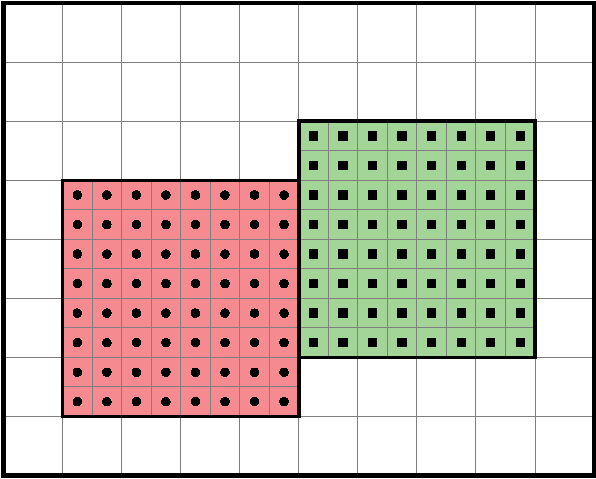
\includegraphics[width=0.9\textwidth]{./Basics/cc_validbox.pdf}
    \caption{\label{fig:basics:cc_validbox} Example of cell-centered valid boxes. There are two
    valid boxes in this example. Each has $8^2$ cells.}
  \end{minipage}\hfill
  \begin{minipage}{0.45\textwidth}
    \centering
    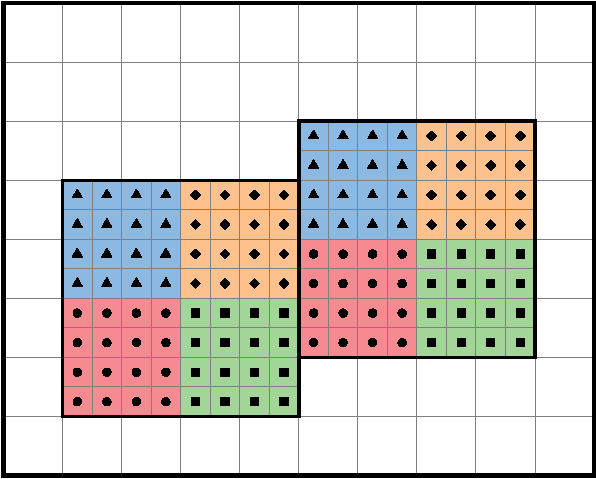
\includegraphics[width=0.9\textwidth]{./Basics/cc_tilebox.pdf}
    \caption{\label{fig:basics:cc_tilebox} Example of cell-centered tile boxes.
      Each grid is {\emph{logically}} broken into 4 tiles, and each
      tile has $4^2$ cells.  There are 8 tiles in total.}
  \end{minipage}
\end{figure}

Figures~\ref{fig:basics:cc_validbox} \& \ref{fig:basics:cc_tilebox}
show an example of the difference between {\tt validbox} and {\tt
  tilebox}.  In this example, there are two grids of cell-centered
index type.  Function {\tt validbox} always return a {\tt Box} for the
valid region of an {\tt FArrayBox} no matter whether or not tiling is
enabled, whereas function {\tt tilebox} returns a {\tt Box} for a
tile.  (Note that when tiling is disabled, {\tt tilebox} returns the
same {\tt Box} as {\tt validbox}.)  The number of loop iteration is 2
in the non-tiling version, whereas in the tiling version the kernel
function is called 8 times.

The tile size can be explicitly set when defining {\tt MFIter}.
\begin{lstlisting}[language=cpp]
  // No tiling in x-direction.
  for (MFIter mfi(mf,IntVect(1024000,16,32)); mfi.isValid(); ++mfi) {...}
\end{lstlisting}
An {\tt IntVect} is used to specify the tile size for every dimension.
A tile size larger than the grid size simply means tiling is disable
in that direction.  \amrex\ has a default tile size {\tt
  IntVect\{1024000,8,8\}} in 3D and no tiling in 2D.  This is used when
tile size is not explicitly set.  One can change the default size
using {\tt ParmParse} parameter {\tt fabarray.mfiter\_tile\_size}.

\begin{figure}
  \centering
  \begin{minipage}{0.45\textwidth}
    \centering
    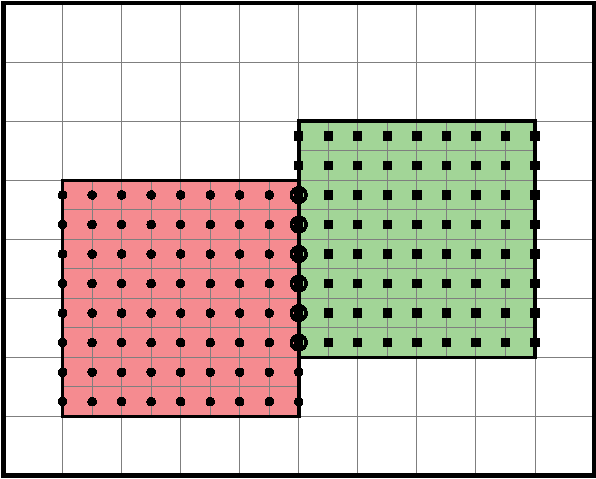
\includegraphics[width=0.9\textwidth]{./Basics/ec_validbox.pdf}
    \caption{\label{fig:basics:ec_validbox} Example of face valid
      boxes. There are two valid boxes in this example. Each has $9
      \times 8$ points.  Note that points in one {\tt Box} may overlap
      with points in the other {\tt Box}.  However, the memory locations
      for storing floating point data of those points do not overlap,
      because they belong to separate {\tt FArrayBox}es.}
  \end{minipage}\hfill
  \begin{minipage}{0.45\textwidth}
    \centering
    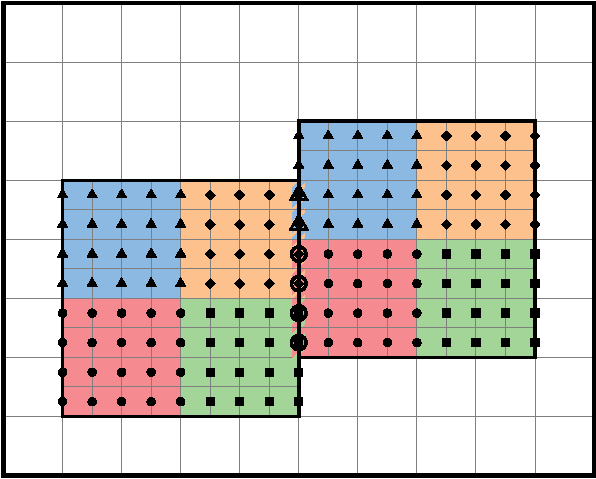
\includegraphics[width=0.9\textwidth]{./Basics/ec_tilebox.pdf}
    \caption{\label{fig:basics:ec_tilebox} Example of face tile boxes.
      Each grid is {\emph{logically}} broken into 4 tiles as indicated
      by the symbols.  There are 8 tiles in total.  Some tiles have $5
      \times 4$ points, whereas others have $4 \times 4$ points.
      Points from different {\tt Box}es may overlap, but points from
      different tiles of the same {\tt Box} do not.}
  \end{minipage}
\end{figure}

Usually {\tt MFIter} is used for accessing multiple {\tt MultiFab}s
like the second example, in which two {\tt MultiFab}s, {\tt U} and
{\tt F}, use {\tt MFIter} via {\tt operator []}.  These different {\tt
  MultiFab}s may have different {\tt BoxArray}s.  For example, {\tt U}
might be cell-centered, whereas {\tt F} might be nodal in
$x$-direction and cell in other directions.  The {\tt
  MFIter::validbox} and {\tt tilebox} functions return {\tt Box}es of
the same type as the {\tt MultiFab} used in defining the {\tt MFIter}
({\tt F} in this example).  Figures~\ref{fig:basics:ec_validbox} \&
\ref{fig:basics:ec_tilebox} show an example of non-cell-centered valid
and tile boxes.  Besides {\tt validbox} and {\tt tilebox}, {\tt
  MFIter} has a number of functions returning various {\tt Box}es.
Examples include,
\begin{lstlisting}[language=cpp]
  Box fabbox() const;       // Return the Box of the FArrayBox

  // Return grown tile box.  By default it grows by the number of
  // ghost cells of the MultiFab used for defining the MFIter.
  Box growntilebox(int ng=-1000000) const;

  // Return tilebox with provided nodal flag as if the MFIter
  // is constructed with MultiFab of such flag.
  Box tilebox(const IntVect& nodal_flag); 
\end{lstlisting} 
It should be noted that function {\tt growntilebox} does not grow the
tile {\tt Box} like a normal {\tt Box}.  Growing a {\tt Box} normally
means the {\tt Box} is extended in every face of every dimension.
However, function {\tt growntilebox} only extends the tile {\tt Box}
in such a way that tiles from the same grid do not overlap.  This is
the basic design principle of these various tiling functions.  Tiling
is a way of domain decomposition for work sharing.  Overlapping tiles
is undesirable because works would be wasted and for multi-threaded
codes race conditions could occur.
Figures~\ref{fig:basics:cc_growbox} \& \ref{fig:basics:ec_growbox}
show examples of {\tt growntilebox}.

\begin{figure}[t]
  \centering
  \begin{minipage}{0.45\textwidth}
    \centering
    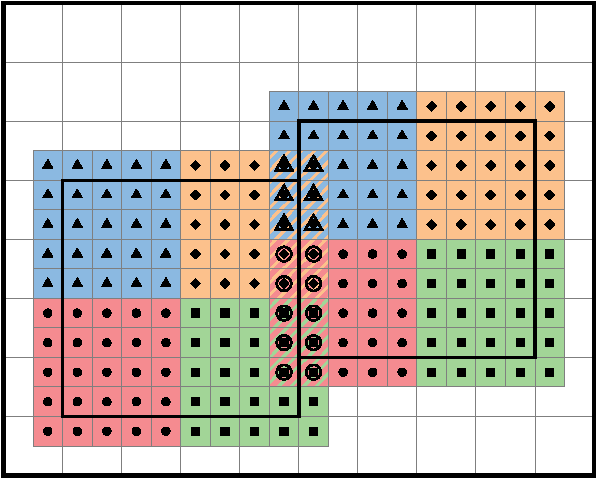
\includegraphics[width=0.9\textwidth]{./Basics/cc_growbox.pdf}
    \caption{\label{fig:basics:cc_growbox} Example of cell-centered
      grown tile boxes. As indicated by symbols, there are 8 tiles and
      four in each grid in this example. Tiles from the same grid do
      not overlap.  But tiles from different grids may overlap.}
  \end{minipage}\hfill
  \begin{minipage}{0.45\textwidth}
    \centering
    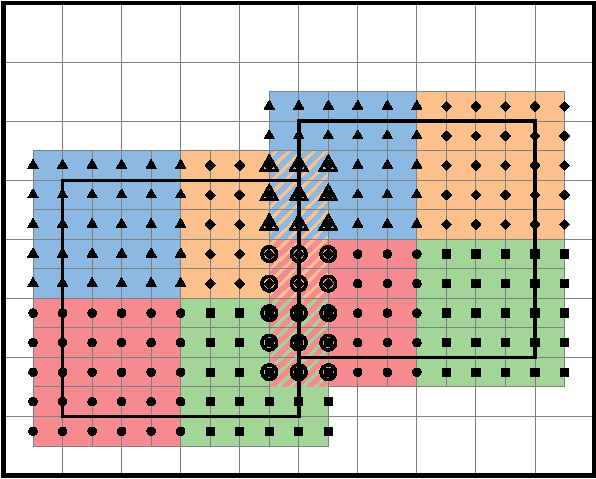
\includegraphics[width=0.9\textwidth]{./Basics/ec_growbox.pdf}
    \caption{\label{fig:basics:ec_growbox} Example of face type grown
      tile boxes.   As indicated by symbols, there are 8 tiles and
      four in each grid in this example. Tiles from the same grid do
      not overlap even though they have face index type. }
  \end{minipage}
\end{figure}

\section{Calling Fortan or C}
\label{sec:basics:fortran}

In Section~\ref{sec:basics:mfiter}, we have shown that a typical
pattern for working with {\tt MultiFab}s is use {\tt MFIter} to
iterate over the data.  In each iteration, a kernel function is called
to work on the data and the work region is specified by a {\tt Box}.
When tiling is used, the work region is a tile.  The tiling is logical
in the sense that there is no data layout transformation.  The kernel
function still gets the whole arrays in {\tt FArrayBox}es, even though
it is supposed to work on a tile region of the arrays.  To \cpp, these
kernel functions are C functions, whose function signatures are
typically declared in a header file named {\tt *\_f.H} or {\tt
  *\_F.H}.  We recommend the users to follow this convention.
Examples of these function declarations are as follows.
\begin{lstlisting}[language=cpp]
  #include <AMReX_BLFort.H>
  #ifdef __cplusplus
  extern "C"
  {
  #endif
      void f1(const int*, const int*, amrex_real*, const int*, const int*);
      void f2(const int*, const int*,
              const amrex_real*, const int*, const int*, const int*
              amrex_real*, const int*, const int*, const int*);
  #ifdef __cplusplus
  }
  #endif
\end{lstlisting}
One can write the functions in C and should include the header
containing the function declarations in the C source code to ensure
type safety.  However, we typically write these kernel functions in
Fortran because of the native multi-dimensional array support.   As we
have seen in Section~\ref{sec:basics:mfiter}, these Fortran functions
take C pointers and view them as multi-dimensional arrays of the shape
specified by the additional integer arguments.  Note that Fortran
takes arguments by reference unless the {\tt value} keyword is used.
So an integer argument on the Fortran side matches an integer pointer
on the \cpp\ side.  Thanks to Fortran 2003, function name mangling is
easily achieved by declaring the Fortran function as {\tt bind(c)}.

\amrex\ provides many macros for passing an {\tt FArrayBox}'s data
into Fortran/C.  For example
\begin{lstlisting}[language=cpp]
  for (MFIter mfi(mf,true); mfi.isValid(); ++mfi)
  {
      const Box& box = mfi.tilebox();
      f(BL_TO_FORTRAN_BOX(box),
        BL_TO_FORTRAN_ANYD(mf[mfi]));
  }
\end{lstlisting}
Here {\tt BL\_TO\_FORTRAN\_BOX} takes a {\tt Box} and provides two
{\tt int*}s specifying the lower and upper bounds of the {\tt Box}.
{\tt BL\_TO\_FORTRAN\_ANYD} takes an {\tt FArrayBox} returned by {\tt
  mf[mfi]} and the preprocessor turns it into {\tt Real*, int*, int*},
where {\tt Real*} is the data pointer that matches real array argument
in Fortran, the first {\tt int*} (which matches an integer argument in
Fortran) specifies the lower bounds, and the second {\tt int*} the
upper bounds of the spatial dimensions of the array.  Similar to we
have seen in Section~\ref{sec:basics:mfiter}, a matching Fortran
function is shown below,
\begin{lstlisting}[language=fortran]
subroutine f(lo, hi, u, ulo, uhi) bind(c)
  use amrex_fort_module, only : amrex_real
  integer, intent(in) :: lo(3),hi(3),ulo(3),uhi(3)
  real(amrex_real),intent(inout)::u(ulo(1):uhi(1),ulo(2):uhi(2),ulo(3):uhi(3))
end subroutine f
\end{lstlisting}
Here, the size of the integer arrays is 3, the maximal number of
spatial dimensions.  If the actual spatial dimension is less than 3,
the degenerate dimensions are set to zero.  So the Fortran function
interface does not have to change according to the spatial
dimensionality, and the bound of the third dimension of the data array
simply becomes {\tt 0:0}.  With the data passed by {\tt
  BL\_TO\_FORTRAN\_BOX} and {\tt BL\_FORTRAN\_ANYD}, this version of
Fortran function interface works for any spatial dimensions.  If one
wants to write a special version just for 2D and would like to use 2D
arrays, one can use
\begin{lstlisting}[language=fortran]
subroutine f2d(lo, hi, u, ulo, uhi) bind(c)
  use amrex_fort_module, only : amrex_real
  integer, intent(in) :: lo(2),hi(2),ulo(2),uhi(2)
  real(amrex_real),intent(inout)::u(ulo(1):uhi(1),ulo(2):uhi(2))
end subroutine f2d
\end{lstlisting}
Note that this does not require any changes in \cpp\ part, because
when \cpp\ passes an integer pointer pointing to an array of three
integers Fortran can treat it as a 2-element integer array.

Another commonly used macro is {\tt BL\_TO\_FORTRAN}.  This macro
takes an {\tt FArrayBox} and provides a real pointer for the floating
point data array and a number of integer pointers for the bounds.
However, the number of the integers depends on the dimensionality.
More specifically, there are 6 and 4 integers for 2D and 3D,
respectively.  The first half of the integers are the lower bounds for
each spatial dimension and the second half the upper bounds.  For
example,
\begin{lstlisting}[language=fortran]
subroutine f2d(u, ulo1, ulo2, uhi1, uhi2) bind(c)
  use amrex_fort_module, only : amrex_real
  integer, intent(in) :: ulo1, ulo2, uhi1, uhi2
  real(amrex_real),intent(inout)::u(ulo1:uhi1,ulo2:uhi2)
end subroutine f2d

subroutine f3d(u, ulo1, ulo2, ulo3, uhi1, uhi2, uhi3) bind(c)
  use amrex_fort_module, only : amrex_real
  integer, intent(in) :: ulo1, ulo2, ulo3, uhi1, uhi2, uhi3
  real(amrex_real),intent(inout)::u(ulo1:uhi1,ulo2:uhi2,ulo3:uhi3)
end subroutine f3d
\end{lstlisting}
Here for simplicity we have omitted passing the tile {\tt Box}.

Usually {\tt MultiFab}s have multiple components.  Thus we often also
need to pass the number of component into Fortran functions.  We can
obtain the number by calling the {\tt MultiFab::nComp()} function, and
pass it to Fortran as we have seen in Section~\ref{sec:basics:mfiter}.
We can also use the {\tt BL\_TO\_FORTRAN\_FAB} macro that is similar
to {\tt BL\_TO\_FORTRAN\_ANYD} except that it provides an additional
{\tt int*} for the number of components.  The Fortran function
matching {\tt BL\_TO\_FORTRAN\_FAB(fab)} is then like below,
\begin{lstlisting}[language=fortran]
subroutine f(u, ulo, uhi,nu) bind(c)
  use amrex_fort_module, only : amrex_real
  integer, intent(in) :: lo(3),hi(3),ulo(3),uhi(3),nu
  real(amrex_real),intent(inout)::u(ulo(1):uhi(1),ulo(2):uhi(2),ulo(3):uhi(3),nu)
end subroutine f
\end{lstlisting}

\section{Boundary}

\amrex\ uses {\tt MultiFab} as the data container for floating point
data on multiple {\tt Box}es on a single AMR level.  Each rectangular
Box has its own boundaries.  A {\tt MultiFab} can have ghost cells for
storing data outside its grid {\tt Box} boundaries.  This allows us to
perform stencil type of operations on regular arrays.  There are three
basic types of boundaries: (1) interior boundary; (2) coarse/fine
boundary; and (3) physical boundary.  Periodic boundary is not
considered a basic type in the discussion here because after periodic
transformation it becomes either interior boundary or coarse/fine
boundary. 

Interior boundary is the border among the grid {\tt Box}es themselves.
For example, in Figure~\ref{fig:basics:amrgrids}, the two blue grid
{\tt Box}es on level 1 share an interior boundary that is 6 cells
long.  For a {\tt MultiFab} with ghost cells on level 1, we can use
the {\tt MultiFab::FillBoundary} function introduced in
Section~\ref{sec:basics:multifab} to fill ghost cells at the interior
boundary with valid cell data from other {\tt Box}es.

Coarse/fine boundary is the border between two AMR levels.  {\tt
FillBoundary} does not fill these ghost cells.  These ghost cells on
the fine level need to be interpolated from the coarse level data.
This is a subject that will be discussed in
Section~\ref{sec:amrcore:fillpatch}. 

The third type of boundary is the physical boundary at the physical
domain.  Note that both coarse and fine AMR levels could have grids
touching the physical boundary.  It is up to the application codes to
properly fill the ghost cells at the physical boundary.
However, \amrex\ does provide support for some common operations.
Here is an example of filling ghost cells at the physical boundary
with first-order extrapolation (i.e., filling the ghost cells with the
data from the last valid cell).
\begin{lstlisting}[language=cpp]
  // mf : MultiFab
  // geom : Geometry
  const Box& domain_box = geom.Domain(); // Box for the whole domain
  for (MFIter mfi(mf); mfi.isValid(); ++mfi)
  {
      FArrayBox& fab = mf[mfi];
      const Box& fab_box = fab.box(); // including ghost cells
      if (!domain_box.contains(fab_box))
      {
          // This FArrayBox touches the domain boundary.
          my_physbc_f();
      }
  }
\end{lstlisting}
\begin{lstlisting}[language=fortran]
  subroutine my_physbc_f(u) bind(c)
    use amrex_fillcc_module, only : amrex_filcc
    call amrex_filcc(u,ulo,uhi...)
  end subroutine my_physbc_f
\end{lstlisting}

\section{I/O}

In this section, we will discuss parallel I/O capabilities for mesh
data in \amrex.  Section~\ref{sec:Particles:IO} will discuss I/O for
particle data.

\subsection{Plotfile}

\amrex\ has its native plotfile format.  Many visualization tools are
available for \amrex\ plotifles
(Chapter~\ref{Chap:Visualization}).  \amrex\ provides the following
two functions for writing a generic \amrex\ plotfile.  Many \amrex\
application codes may have their own plotifile routines that store
additional information such as compiler options, git hashes of the
source codes and {\tt ParmParse} runtime parameters.
\begin{lstlisting}[language=cpp]
  void WriteSingleLevelPlotfile (const std::string &plotfilename,
                                 const MultiFab &mf,
                                 const Array<std::string> &varnames,
                                 const Geometry &geom,
                                 Real time,
                                 int level_step);

  void WriteMultiLevelPlotfile (const std::string &plotfilename,
                                int nlevels,
                                const Array<const MultiFab*> &mf,
                                const Array<std::string> &varnames,
                                const Array<Geometry> &geom,
                                Real time,
                                const Array<int> &level_steps,
                                const Array<IntVect> &ref_ratio);
\end{lstlisting}
{\tt WriteSingleLevelPlotfile} is for single level runs and {\tt
WriteMultiLevelPlotfile} is for multiple levels.  The name of the
plotfile is specified by the `plotfilename` argument.  This is the
directory name and for the plotfile.  In \amrex\ convention, the
plotfile name consist of letters followed by numbers (e.g., {\tt
plt00258}).  {\tt amrex::Concatenate} is a useful helper function for
making such strings,
\begin{lstlisting}[language=cpp]
  int istep = 258;
  const std::string& pfname = amrex::Concatenate("plt",istep); // plt00258

  // By default there are 5 digits, but we can change it to say 4.
  const std::string& pfname2 = amrex::Concatenate("plt",istep,4); // plt0258  

  istep =1234567;  // Having more than 5 digits is OK.
  const std::string& pfname3 = amrex::Concatenate("plt",istep); // plt12344567
\end{lstlisting}
Argument {\tt mf} ({\tt MultiFab} for single level and {\tt
Array<const Multifab*} for multi-level) is the data to be written to
the disk.  Note that many visualization tools expect this to be
cell-centered data.  So for nodal data, we need to convert them
cell-centered data through some kind of averaging.  Also note that if
you have data at each AMR level in several {\tt MulitiFab}s, you need
to build a new {\tt MultiFab} at each level to hold all the data.
This involves local data copy in memory and is not expected to
increase the total wall time for writing data to the disk.  For the
multi-level version, the function expects {\tt Array<const
MultiFab*>}, whereas the multi-level data are often stored as {\tt
Array<std::unique\_ptr<MultiFab>>}.  \amrex\ has a helper function for
this and one can use it as follows,
\begin{lstlisting}[language=cpp]
   WriteMultiLevelPlotfile(......, amrex::GetArrOfConstPtrs(mf), ......);
\end{lstlisting}
Argument {\tt varnames} has the names for each component of the {\tt
MultiFab} data.  The size of the {\tt Array} should be equal to the
number of components.  Argument {\tt geom} is for passing {\tt
Geometry} objects that contain the physical domain
information. Argument {\tt time} is for the time associated with the
data.  Argument {\tt level\_step} is for the current time step
associated with the data.  For multi-level plotfiles, argument {\tt
nlevels} is the total number of levels, and we also need to provide
the refinement ratio via an {\tt Array} of size {\tt nlevels-1}.

We note that \amrex\ does not overwrite old plotfiles if the new
plotfile has the same name.  The old plotfiles will be renamed to
new directories named like {\tt plt00350.old.46576787980}.

\subsection{Checkpoint File}

Checkpoint files are used for restarting simulations from where the
checkpoints are written.  Each application code has its own set of
data needed for restart.  \amrex\ provides I/O functions for basic
data structures like {\tt MultiFab} and {\tt BoxArray}.  These
functions can be used to build codes for reading and writing
checkpoint files.  Since each application code has its own
requirement, there is no standard \amrex\ checkpoint format.

Typically a checkpoint file is a directory containing some text files
and sub-directories (e.g., {\tt Level\_0} and {\tt Level\_1}).  For
example, to build directories {\tt chk00016}, {\tt chk00016/Level\_0},
and {\tt chk00016/Level\_1}, we do
\begin{lstlisting}[language=cpp]
  const std::string& chkname {"chk00016"};
  const std::string& subDirPrefix {"Level_"};
  const int nSubDirs = 2;
  const bool callBarrier = true; // Parallel barrier after directories are built.
  PreBuildDirectorHierarchy(chkname, subDirPrefix, nSubDirs, callBarrier);
\end{lstlisting}

A checkpoint file of \amrex\ application codes often has a clear text
{\tt Header} file that only the I/O process writes to it using {\tt
std::ofstream}.  The {\tt Header} file contains information such as
the time, the physical domain size, grids, etc. that are necessary for
restarting the simulation.  To guarantee that precision is not lost
for storing floating point number like time in clear text file, the
file stream's precision needs to be set properly.  And a stream buffer
can also be used.  For example,
\begin{lstlisting}[language=cpp]
  if (ParallelDescriptor::IOProcessor())
  {
      const std::string& chkname = "chk00016";
      std::string HeaderFileName(chkname+"/Header");
      std::ofstream HeaderFile(HeaderFileName.c_str(),
           std::ofstream::out | std::ofstream::trunc | std::ofstream::binary);
      HeaderFile.precision(std::numeric_limits<Real>::max_digits10);
      VisMF::IO_Buffer io_buffer(VisMF::IO_Buffer_Size);
      HeaderFile.rdbuf()->pubsetbuf(io_buffer.dataPtr(), io_buffer.size());

      HeaderFile << "Checkpoint version 1.0\n";
      HeaderFile << time << "\n";
      HeaderFile << domain_box << "\n";
      // HeaderFile << ......;
      box_array.writeOn(HeaderFile); // write BoxArray
      // HeaderFile << ......;
  }
\end{lstlisting}
For reading the {\tt Header} file, \amrex\ can have the I/O process
read the file from the disk and broadcast it to others as {\tt
Array<char>}.  Then all processes can read the information with {\tt
std::istringstream}.  For example,
\begin{lstlisting}[language=cpp]
  std::string HeaderFileName {"chk00016/Header"};
  Array<char> fileChar;
  ParallelDescriptor::ReadAndBcastFile(HeaderFileName, fileChar);
  std::istringstream is(std::string{fileChar.data()}, std::istringstream::in);
  // is >> ....;
  BoxArray ba;
  ba.readFrom(is);
  // is >> ....;
\end{lstlisting}

{\tt amrex::VisMF} is a class that can be used to perform parallel
read and write {\tt MultiFab}s on the disk.  How many processes are
allowed to perform I/O simultaneously can be set via
\begin{lstlisting}[language=cpp]
  VisMF::SetNOutFiles(64);  // up to 64 processes, which is also the default.
\end{lstlisting}
The optimal number is of course system dependent.  The following code
shows how to write and read a {\tt MultiFab}.
\begin{lstlisting}[language=cpp]
  const std::string name {"state"};

  VisMF::Write(mf, name);  // Write MultiFab to disk

  // Read the data to a new MultiFab
  // WARNING: mf2 may have a completely different DistributionMapping!
  MultiFab mf2;
  VisMF::Read(mf2, name);

  // Read the data to a new MultiFab with identical
  // BoxArray, DistributionMapping, and number of components and ghost cells.
  MultiFab mf3(mf.boxArray(), mf.DistributionMap(), mf.nComp(), mf.nGrow());
  VisMF::Read(mf3, name);
\end{lstlisting}
It should be emphasized that calling {\tt VisMF::Read} with an empty
{\tt MultiFab} (i.e., no memory allocated for floating point data)
will result in a {\tt MuitiFab} with a new {\tt DistributionMapping}
that could be different from any other existing {\tt
DistributionMapping} objects.  It should also be noted that all the
data including those in ghost cells are written/read by {\tt
VisMF::Write/Read}. 

\section{Memory Allocation}

\amrex\ has a Fortran module, {\tt mempool\_module} that can be used to
allocate memory for Fortran pointers.  The reason that such a module
exists in \amrex\ is memory allocation is often very slow in
multi-threaded OpenMP parallel regions.  \amrex\ {\tt mempool\_module}
provides a much faster alternative approach, in which each thread has
its own memory pool.  Here are examples of using the module.
\begin{lstlisting}[language=fortran]
  use mempool_module, only : bl_allocate, bl_deallocate
  real(amrex_real), pointer, contiguous :: a(:,:,:), b(:,:,:,:)
  integer :: lo1, hi1, lo2, hi2, lo3, hi3, lo(4), hi(4)
  // lo1 = ...
  // a(lo1:hi1, lo2:hi2, lo3:hi3)
  call bl_allocate(a, lo1, hi1, lo2, hi2, lo3, hi3)
  // b(lo(1):hi(1),lo(2):hi(2),lo(3):hi(3),lo(4):hi(4))
  call bl_allocate(b, lo, hi)
  // ......
  call bl_deallocate(a)
  call bl_deallocate(b)
\end{lstlisting}
The downside of this is we have to use {\tt pointer} instead of {\tt
allocatable}.  This means we must explicitly free the memory via {\tt
bl\_deallocate} and we need to declare the pointers as {\tt
contiguous} for performance reason.

\section{Abort and Assertion}

{\tt amrex::Abort(const char* message)} is used to terminate a run
usually when something goes wrong.  This function takes a message and
write it to stderr.  Files named like {\tt Backtrace.rg\_1\_rl\_1}
(where {\tt rg\_1\_rl\_1} means process \# 1) are produced containing
backtrace information of the call stack.  In Fortran, we can call {\tt
amrex\_abort} from the {\tt amrex\_error\_module}, which takes a
Fortran {\tt character} variable with assumed size (i.e., {\tt len=*})
as a message.

{\tt AMREX\_ASSERT} is a macro that takes a Boolean expression.  For
debug build (e.g., {\tt DEBUG=TRUE} using the GNU Make build system),
if the expression at runtime is evaluated to false, {\tt amrex::Abort}
will be called and the run is thus terminated.  For optimized build
(e.g., {\tt DEBUG=TRUE} using the GNU Make build system), the {\tt
AMREX\_ASSERT} statement is removed at compile time and thus has no
effect at runtime.  We often use this as a means of putting debug
statement in the code without adding any extra cost for production
runs.  For example,
\begin{lstlisting}[language=cpp]
  AMREX_ASSERT(mf.nGrow() > 0 && mf.nComp() == mf2.nComp());
\end{lstlisting}
Here for debug build we like to assert that {\tt MultiFab} {\tt mf}
has ghost cells and it also has the same number of components as {\tt
MultiFab} {\tt mf2}.  If we always want the assertion, we can use {\tt
AMREX\_ALWAYS\_ASSERT}.


\chapter{Boundary Conditions}\label{Chap:Boundary}
This chapter describes how to implement domain boundary conditions in \amrex.
A ghost cell that is outside of the valid region can be thought of as either
``interior'' (for periodic and coarse-fine ghost cells), or ``physical''.
Physical boundary conditions can include inflow, outflow, slip/no-slip walls,
but are ultimately linked to mathematical Dirichlet or Neumann conditions.

The basic idea behind physical boundary conditions is as follows:
\begin{itemize}

\item Create a {\tt BCRec} object, which is essentially a multidimensional integer array of
{\tt 2*DIM} components.  Each component defines a boundary condition type for
the lo/hi side of the domain, for each direction.
See {\tt Src/Base/AMReX\_BC\_TYPES.H} for common physical and mathematical types.
If there is more than one variable, we can create an array of {\tt BCRec} objects,
and pass in a pointer to the 0-index component since the arrays for all the 
components are contiguous in memory.
Here we need to provide boundary types to each component of the {\tt
MultiFab}.  Below is an example of setting up {\tt Vector<BCRec>}
before the call to ghost cell routines.
\begin{lstlisting}[language=cpp]
  // Set up BC; see Src/Base/AMReX_BC_TYPES.H for supported types
  Vector<BCRec> bc(phi.nComp());
  for (int n = 0; n < phi.nComp(); ++n)
  {
      for (int idim = 0; idim < AMREX_SPACEDIM; ++idim)
      {
          if (Geometry::isPeriodic(idim))
          {
              bc[n].setLo(idim, BCType::int_dir); // interior
              bc[n].setHi(idim, BCType::int_dir);
          }
          else
          {
              bc[n].setLo(idim, BCType::foextrap); // first-order extrapolation
              bc[n].setHi(idim, BCType::foextrap);
          }
      }
  }
\end{lstlisting}
{\tt amrex::BCType} has the following types,
\begin{quote}
\begin{description}
\item [int\_dir] Interior, including periodic boundary
\item [ext\_dir] ``External Dirichlet''.  It is the user's responsibility to write a routine
to fill ghost cells (more details below).
\item [foextrap] ``First Order Extrapolation'' 
First order extrapolation from last cell in interior.
\item [reflect\_even] Reflection from interior cells with sign
  unchanged, $q(-i) = q(i)$.
\item [reflect\_odd] Reflection from interior cells with sign
  unchanged, $q(-i) = -q(i)$.
\end{description}
\end{quote}

\item We have interfaces to a fortran routine that fills ghost cells at domain
boundaries based on the boundary condition type defined in the {\tt BCRec} object.
It is the user's responsibility to have a consisent definition of what the ghost cells
represent.  A common option used in \amrex\ codes is to fill the domain ghost cells
with the value that lies on the boundary (as opposed to another common option where
the value in the ghost cell represents an extrapolated value based on the boundary
condition type).  Then in our stencil based ``work'' codes, we also pass in the
{\tt BCRec} object and use modified stencils near the domain boundary that know the value
in the first ghost cell represents the value on the boundary.

\end{itemize}

Depending on the level of complexity of your code, there are various options
for filling domain boundary ghost cells.

For single-level codes built from {\tt Src/Base} (excluding the 
{\tt Src/AmrCore} and {\tt Src/Amr} source code directories), you will have 
single-level {\tt MultiFab}s filled with data in the valid region where you need 
to fill the ghost cells on each grid.  There are essentially three ways to fill the ghost 
cells. (refer to Tutorials/Basic/HeatEquation\_EX2\_C for an example).

\begin{lstlisting}[language=cpp]
MultiFab mf;
Geometry geom;
Vector<BCRec> bc;

// ...

// fills interior and periodic domain boundary ghost cells
mf.FillBoundary(geom.periodicity());

// fills interior (but not periodic domain boundary) ghost cells
mf.FillBoundary();

// fills physical domain boundary ghost cells
FillDomainBoundary(mf, geom, bc);
\end{lstlisting}

{\tt FillDomainBoundary()} is a function is in {\tt Src/Base/AMReX\_BCUtil.cpp},
and is essentially an interface to fortran {\tt subroutine amrex\_fab\_filcc()}
in {\tt Src/Base/AMReX\_filcc\_mod.F90}, which ultimately calls fortran 
{\tt subroutine filcc()} in {\tt Src/Base/AMReX\_FILCC\_XD.F}.  To create more
custom boundary conditions, create a local modified copy of
{\tt Src/Base/AMReX\_FILCC\_XD.F} and put it your local source code.

For multi-level codes using the {\tt Src\_AmrCore} source code, the
functions described above still work, however additional classes need to
be set up since the {\tt FillPatch} routines call them.
In fact it is possible to avoid using the single-level calls directly if
you fill all your grids and ghost cells using the {\tt FillPatch} routines.
Refer to {\tt Tutorials/Amr/Advection\_AmrCore/} for an example.
The class {\tt PhysBCFunct} in {\tt Src/Base/AMReX\_PhysBCFunct.cpp}
is derived from {\tt PhysBCFunctBase} and contains a {\tt BCRec}, {\tt Geometry},
and a pointer to a {\tt BndryFunctBase} function.

The function {\tt FillBoundary} fills physical ghost cells (so it has a different
functionality from the single-level case described above, where {\tt FillDomainBoundary}
fills the physical ghost cells).


\chapter{{\tt AmrCore} Source Code}\label{Chap:AmrCore}
In this Chapter we give an overview of functionality contained in the {\tt amrex/Src/AmrCore} source code.
This directory contains source code for the following:
\begin{itemize}
\item Storing information about the grid layout and processor distribution mapping
at each level of refinement.
\item Functions to create grids at different levels of refinement, including tagging
operationrs.
\item Operations on data at different levels of refinement, such as interpolation and
restriction operators.
\item Flux registers used to store and manipulate fluxes at coarse-fine interfaces.
\item Particle support for AMR.
\end{itemize}
There is another source directory, {\tt amrex/Src/Amr/}, which contains
additional classes used to manage the time-stepping for AMR simulations.
However, it is possible to build a fully adaptive, subcycling-in-time simulation code
without these additional classes.

In this Chapter, we restrict our use to the {\tt amrex/Src/AmrCore} source code
and present a tutorial that performs an adaptive, subcycling-in-time simulation
of the advection equation for a passively advected scalar.
The accompanying tutorial code is available in {\tt amrex/Tutorials/Amr/Advection\_AmrCore}
with build/run directory {\tt Exec/SingleVortex}.  In this example, a Gaussian profile is
initially displaced but returns to its original configuration at the final time.
The boundary conditions are periodic and we use a refinement ratio of $r=2$ between each AMR level.
The results of the simulation are depicted in Figure \ref{fig:Adv}.
\begin{figure}
  \centering
  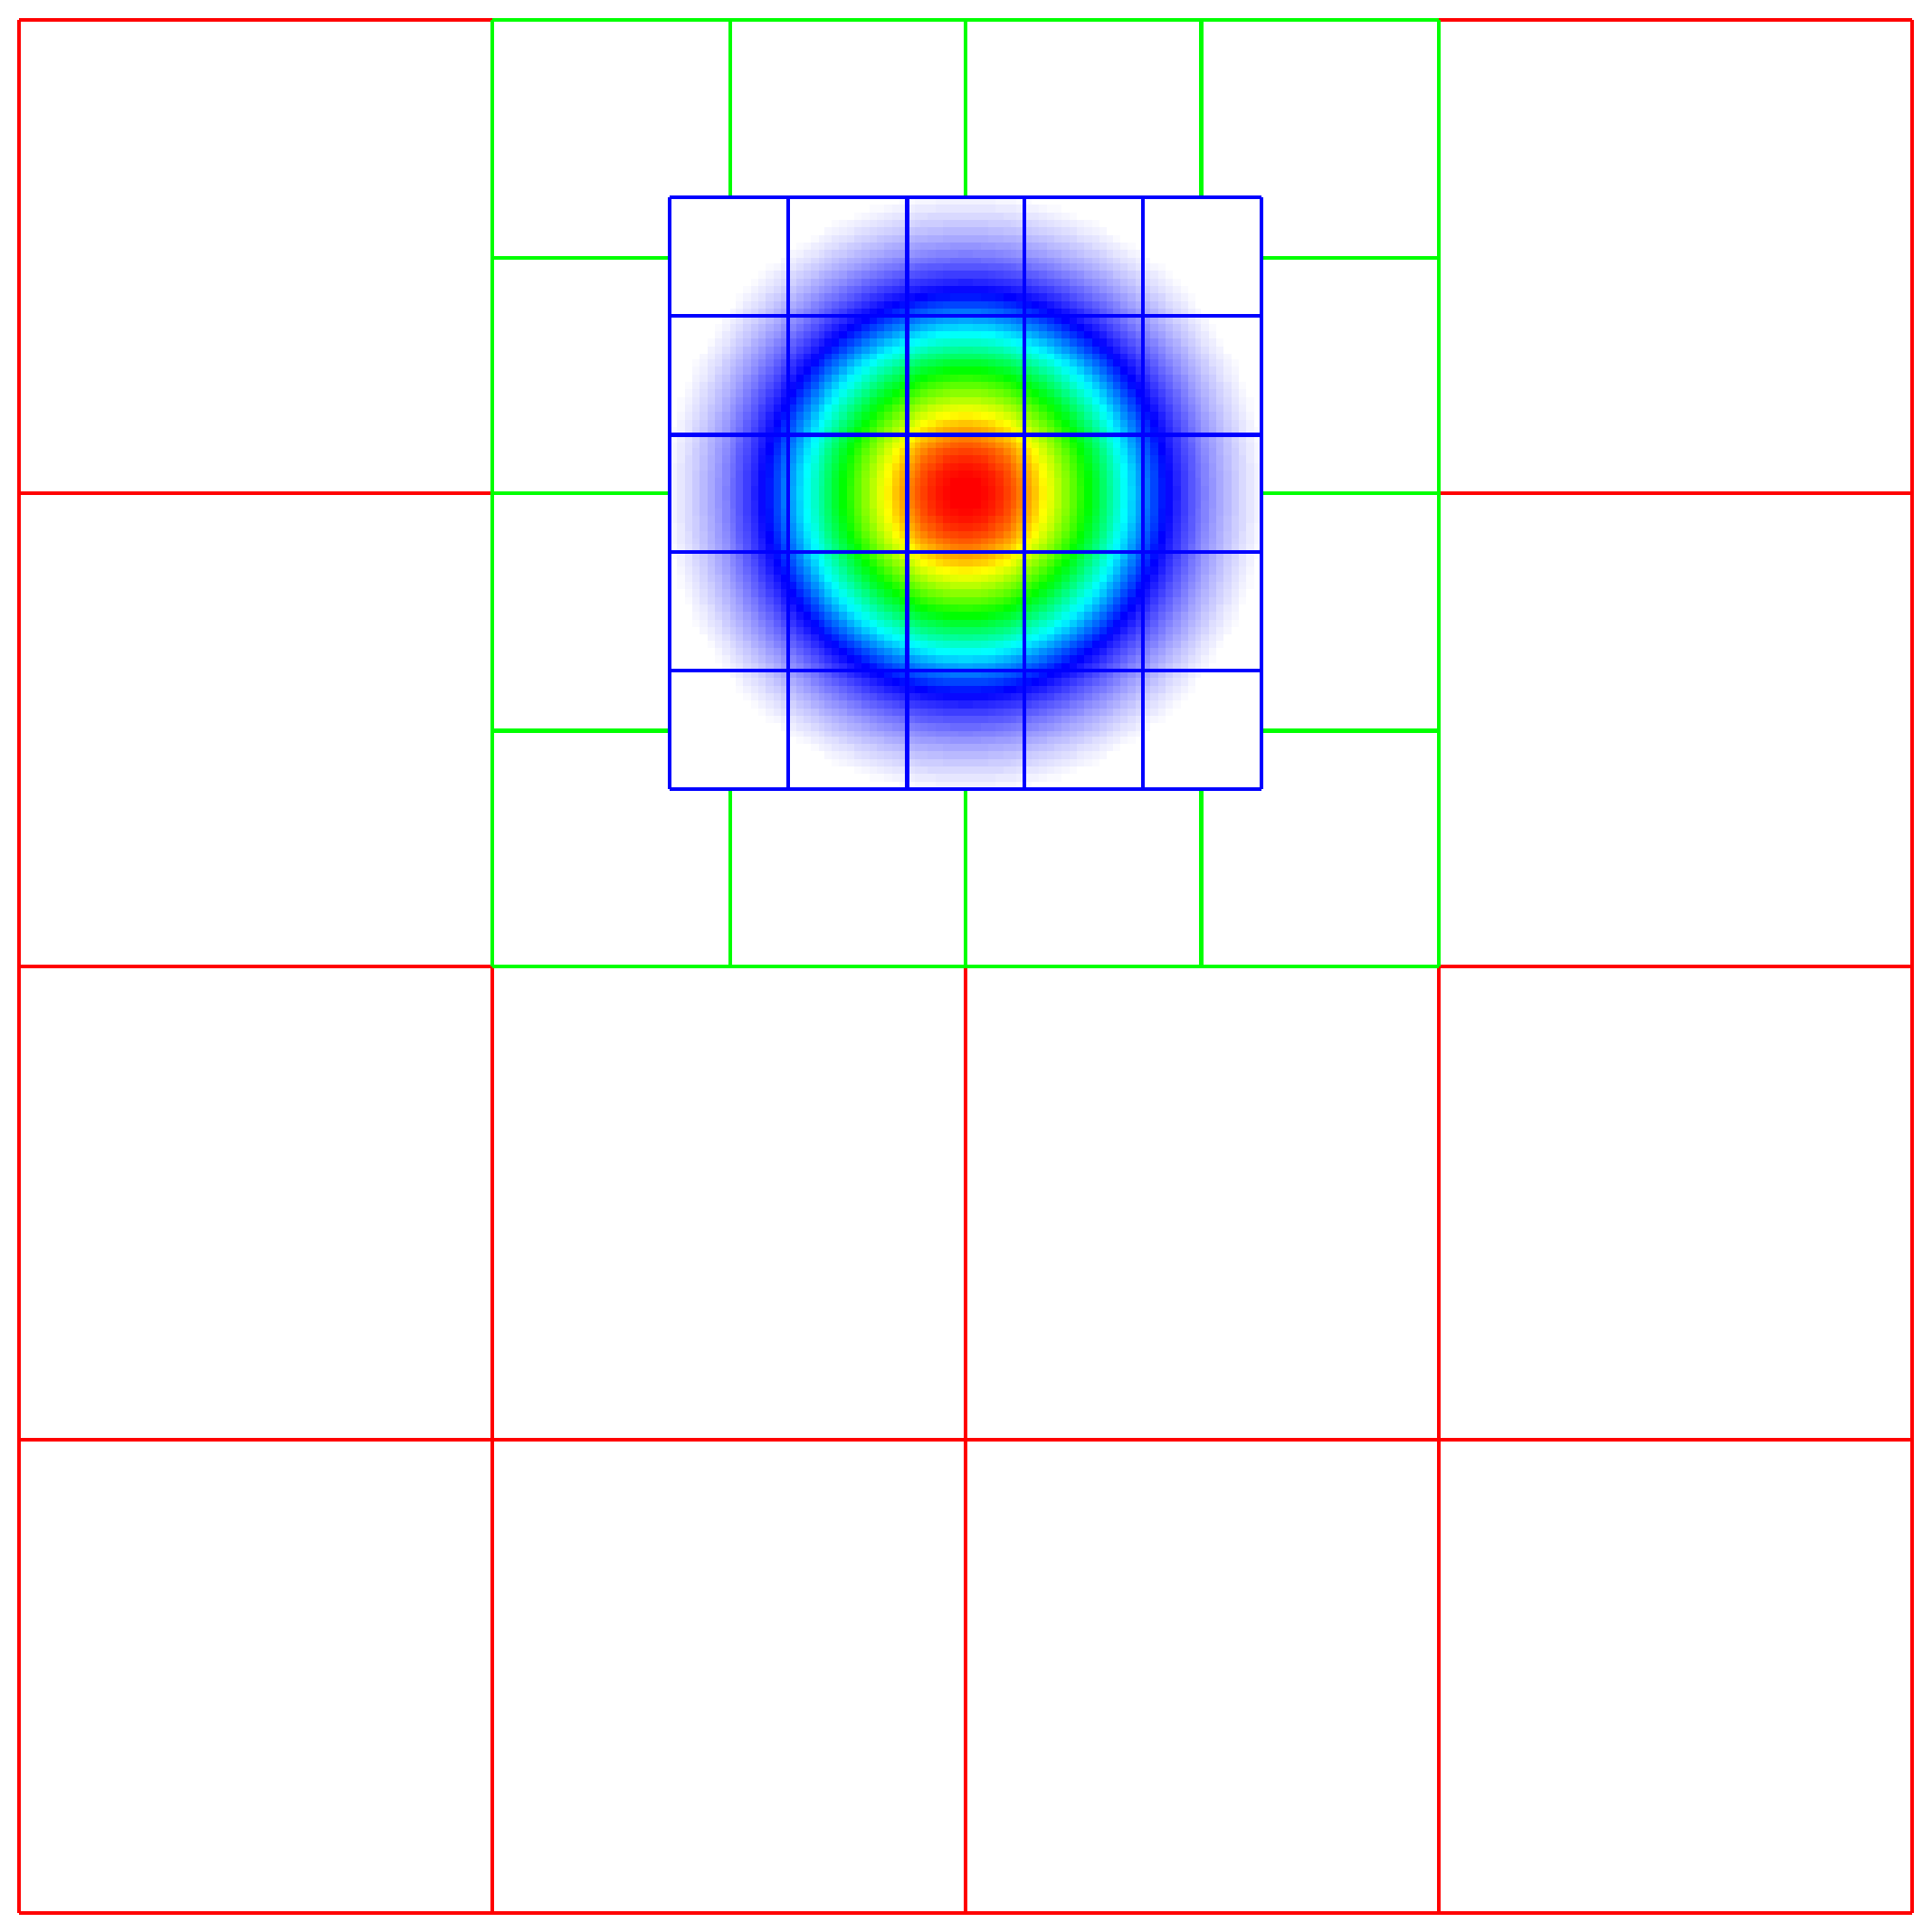
\includegraphics[width=1in]{./AmrCore/figs/Adv1.pdf}
  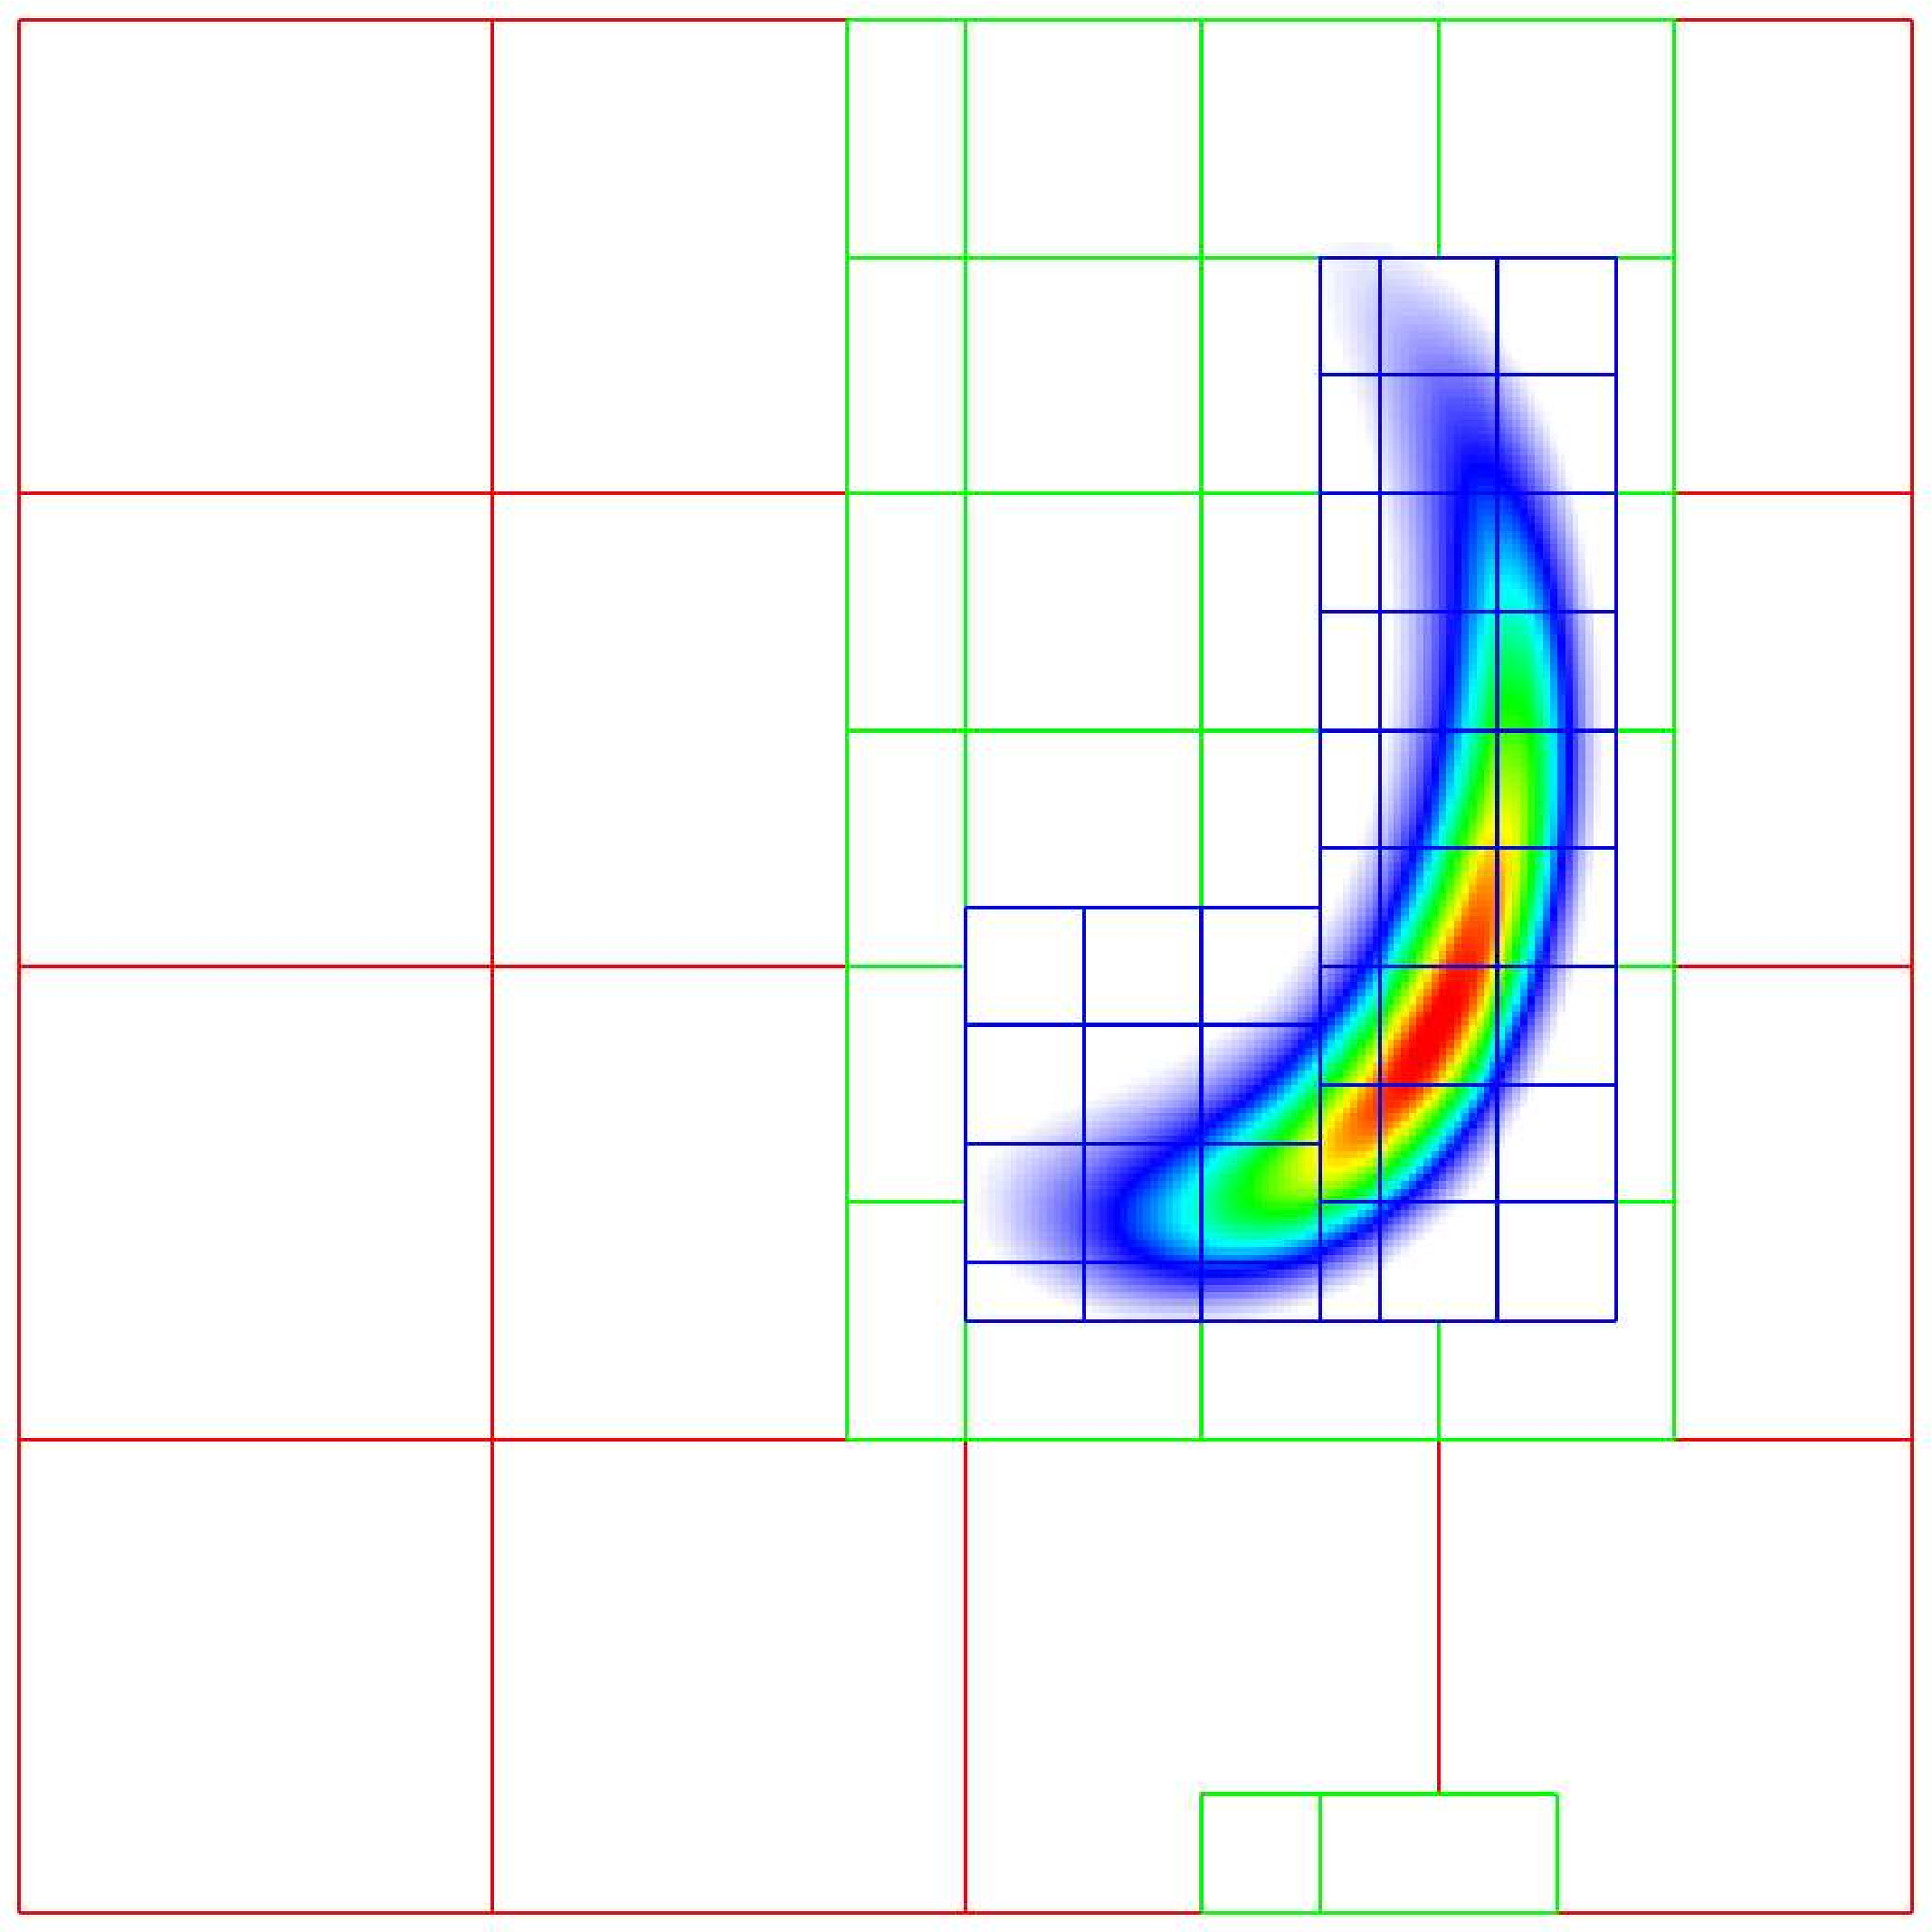
\includegraphics[width=1in]{./AmrCore/figs/Adv2.pdf}
  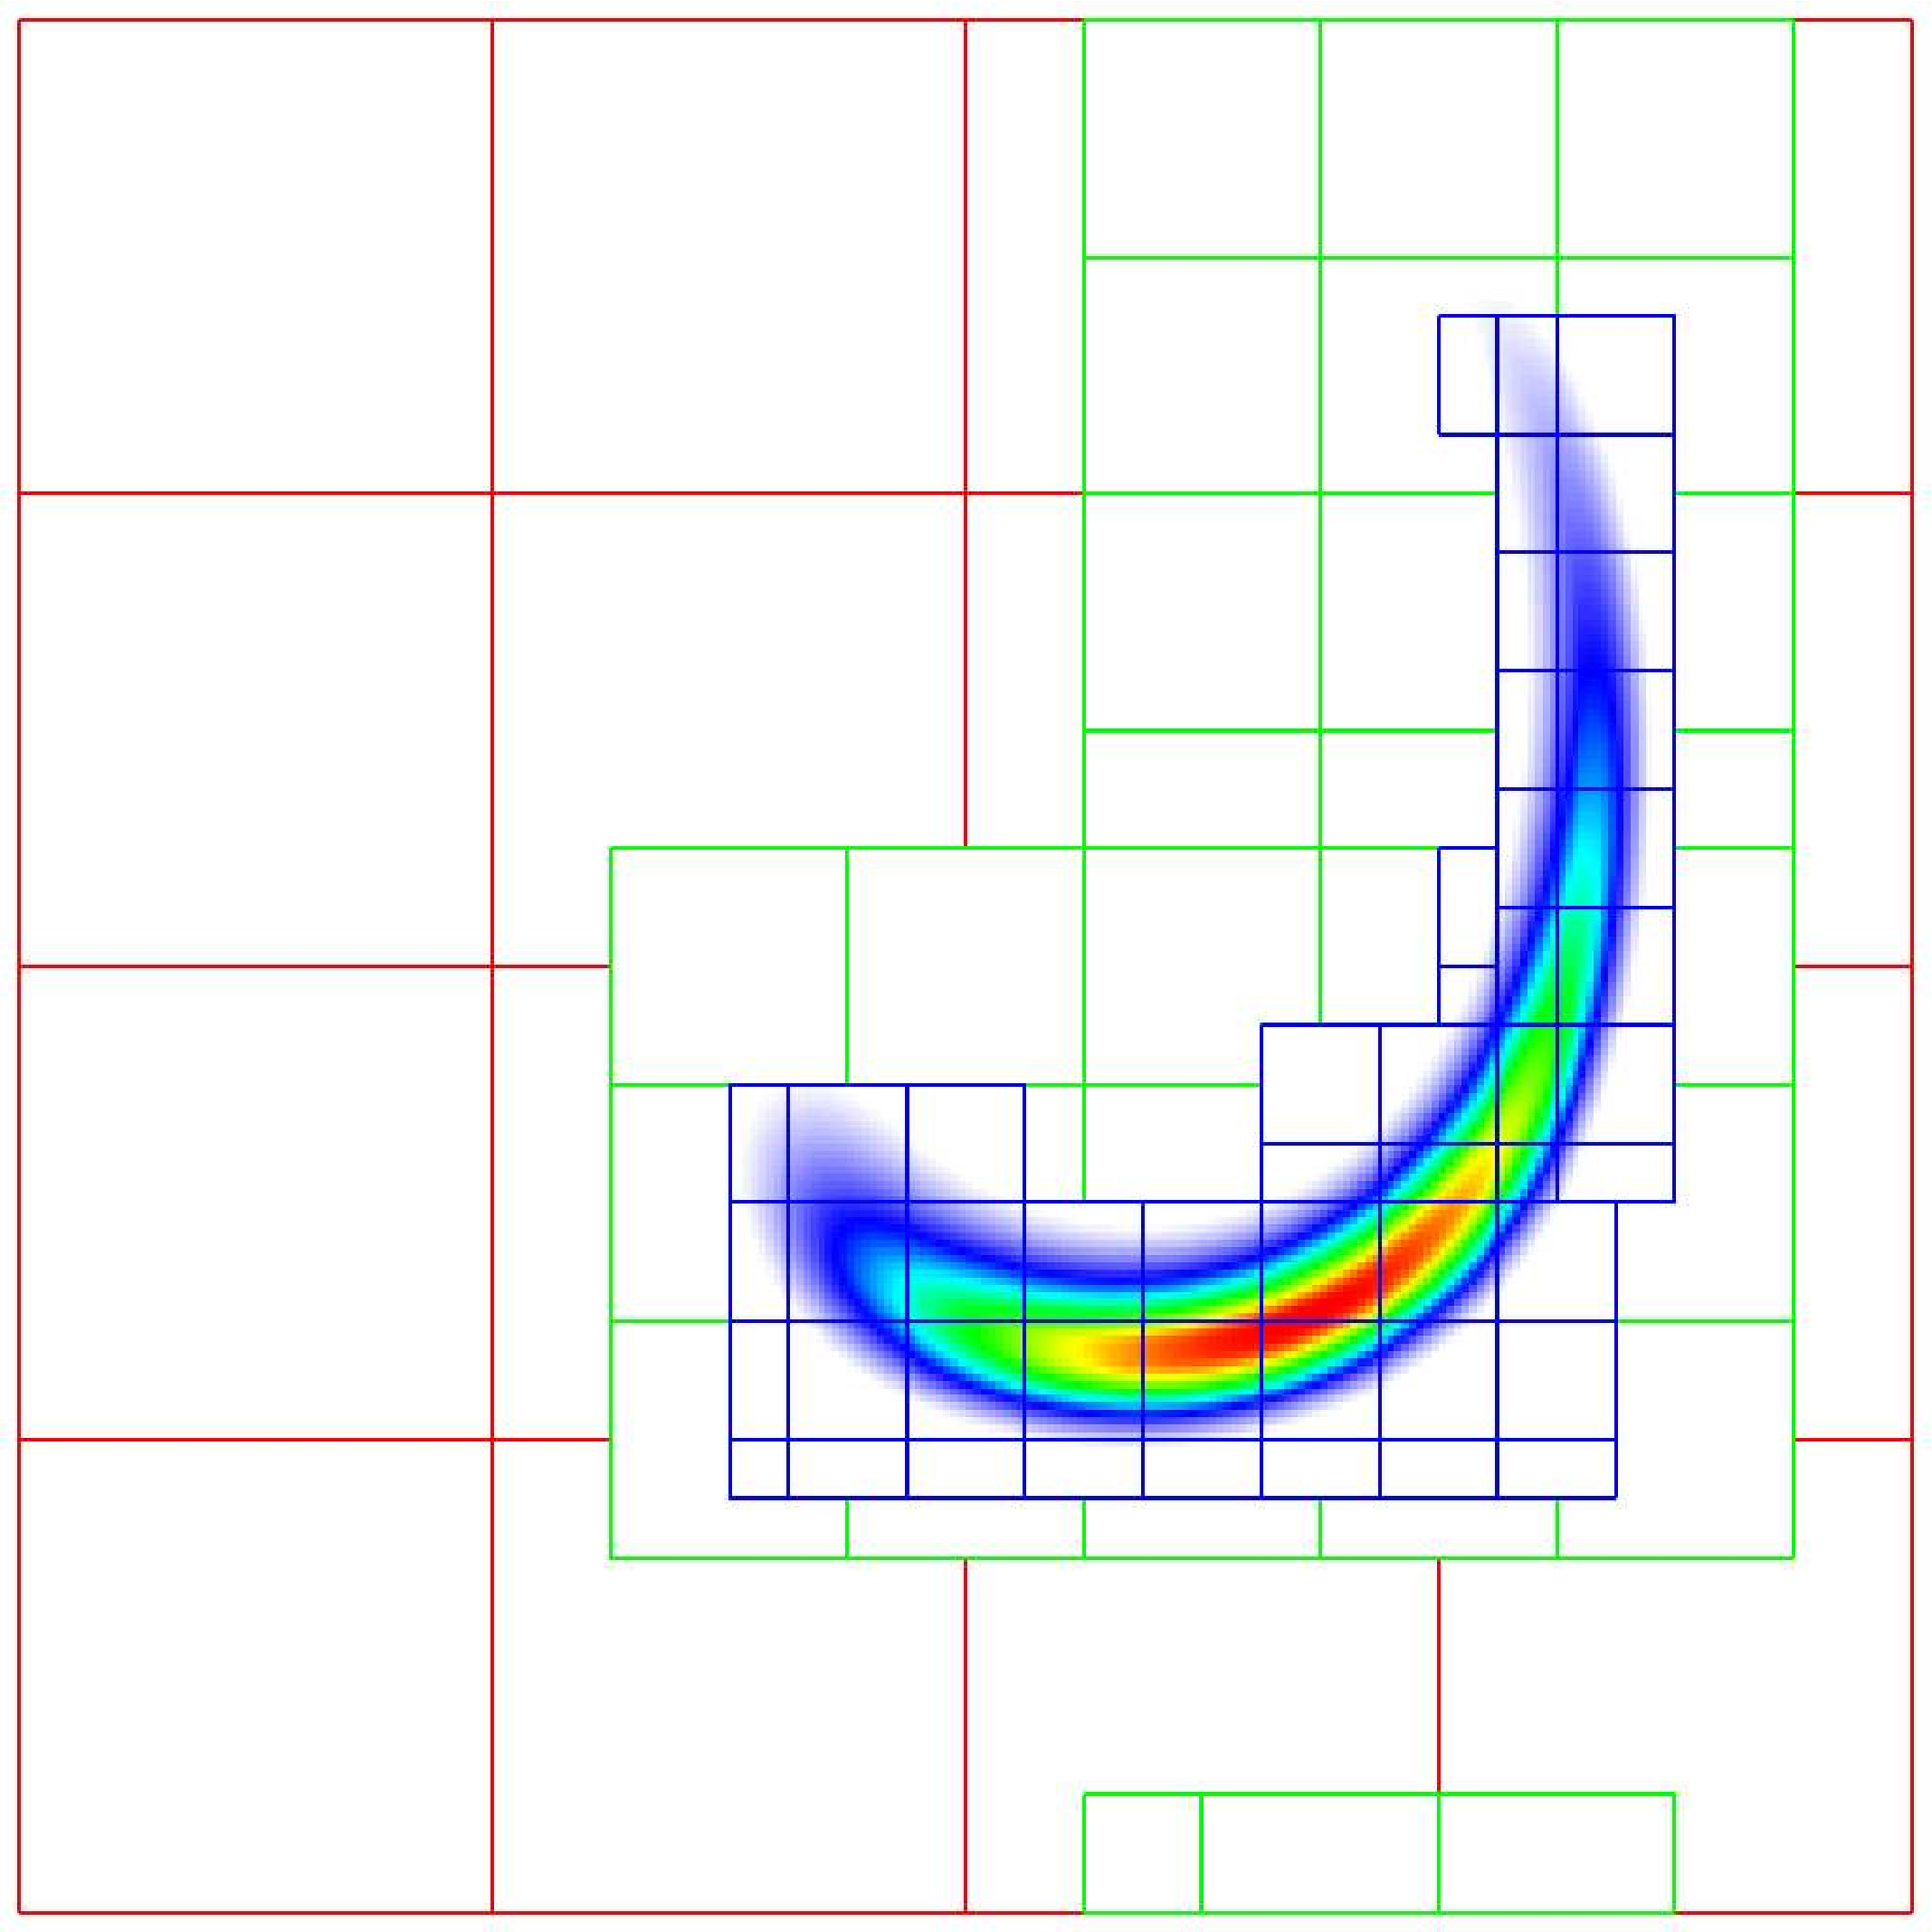
\includegraphics[width=1in]{./AmrCore/figs/Adv3.pdf}
  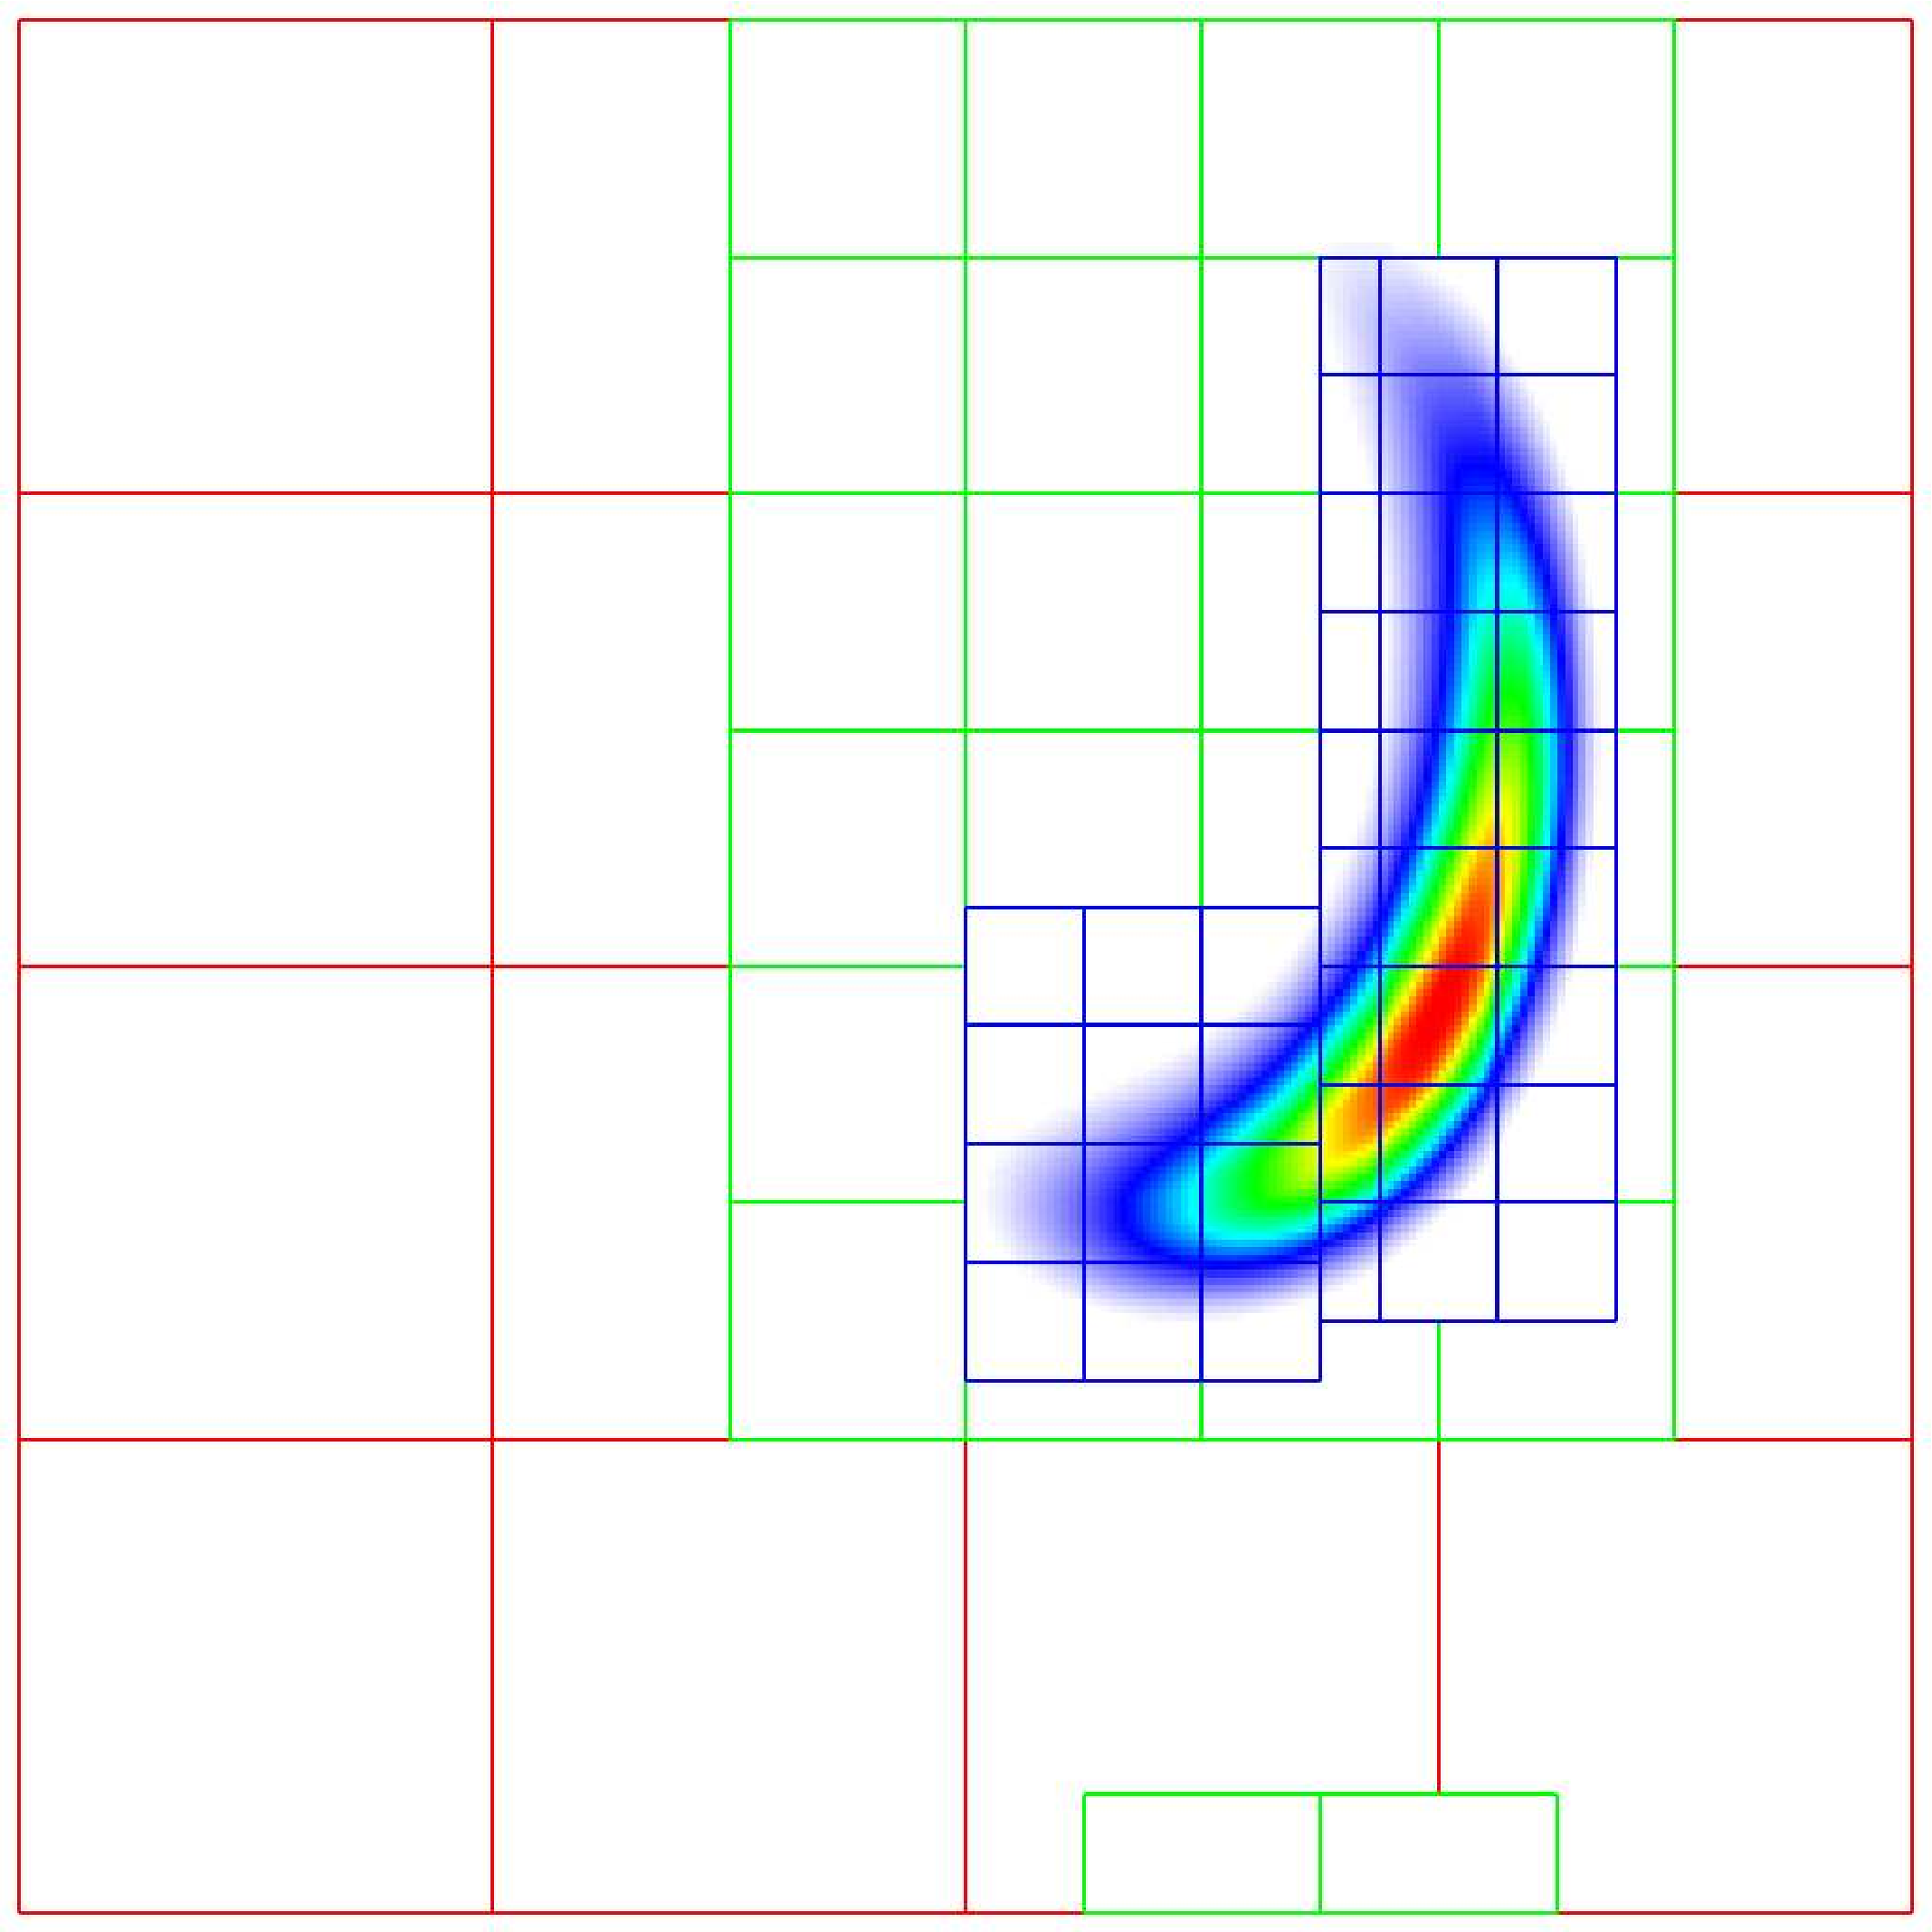
\includegraphics[width=1in]{./AmrCore/figs/Adv4.pdf}
  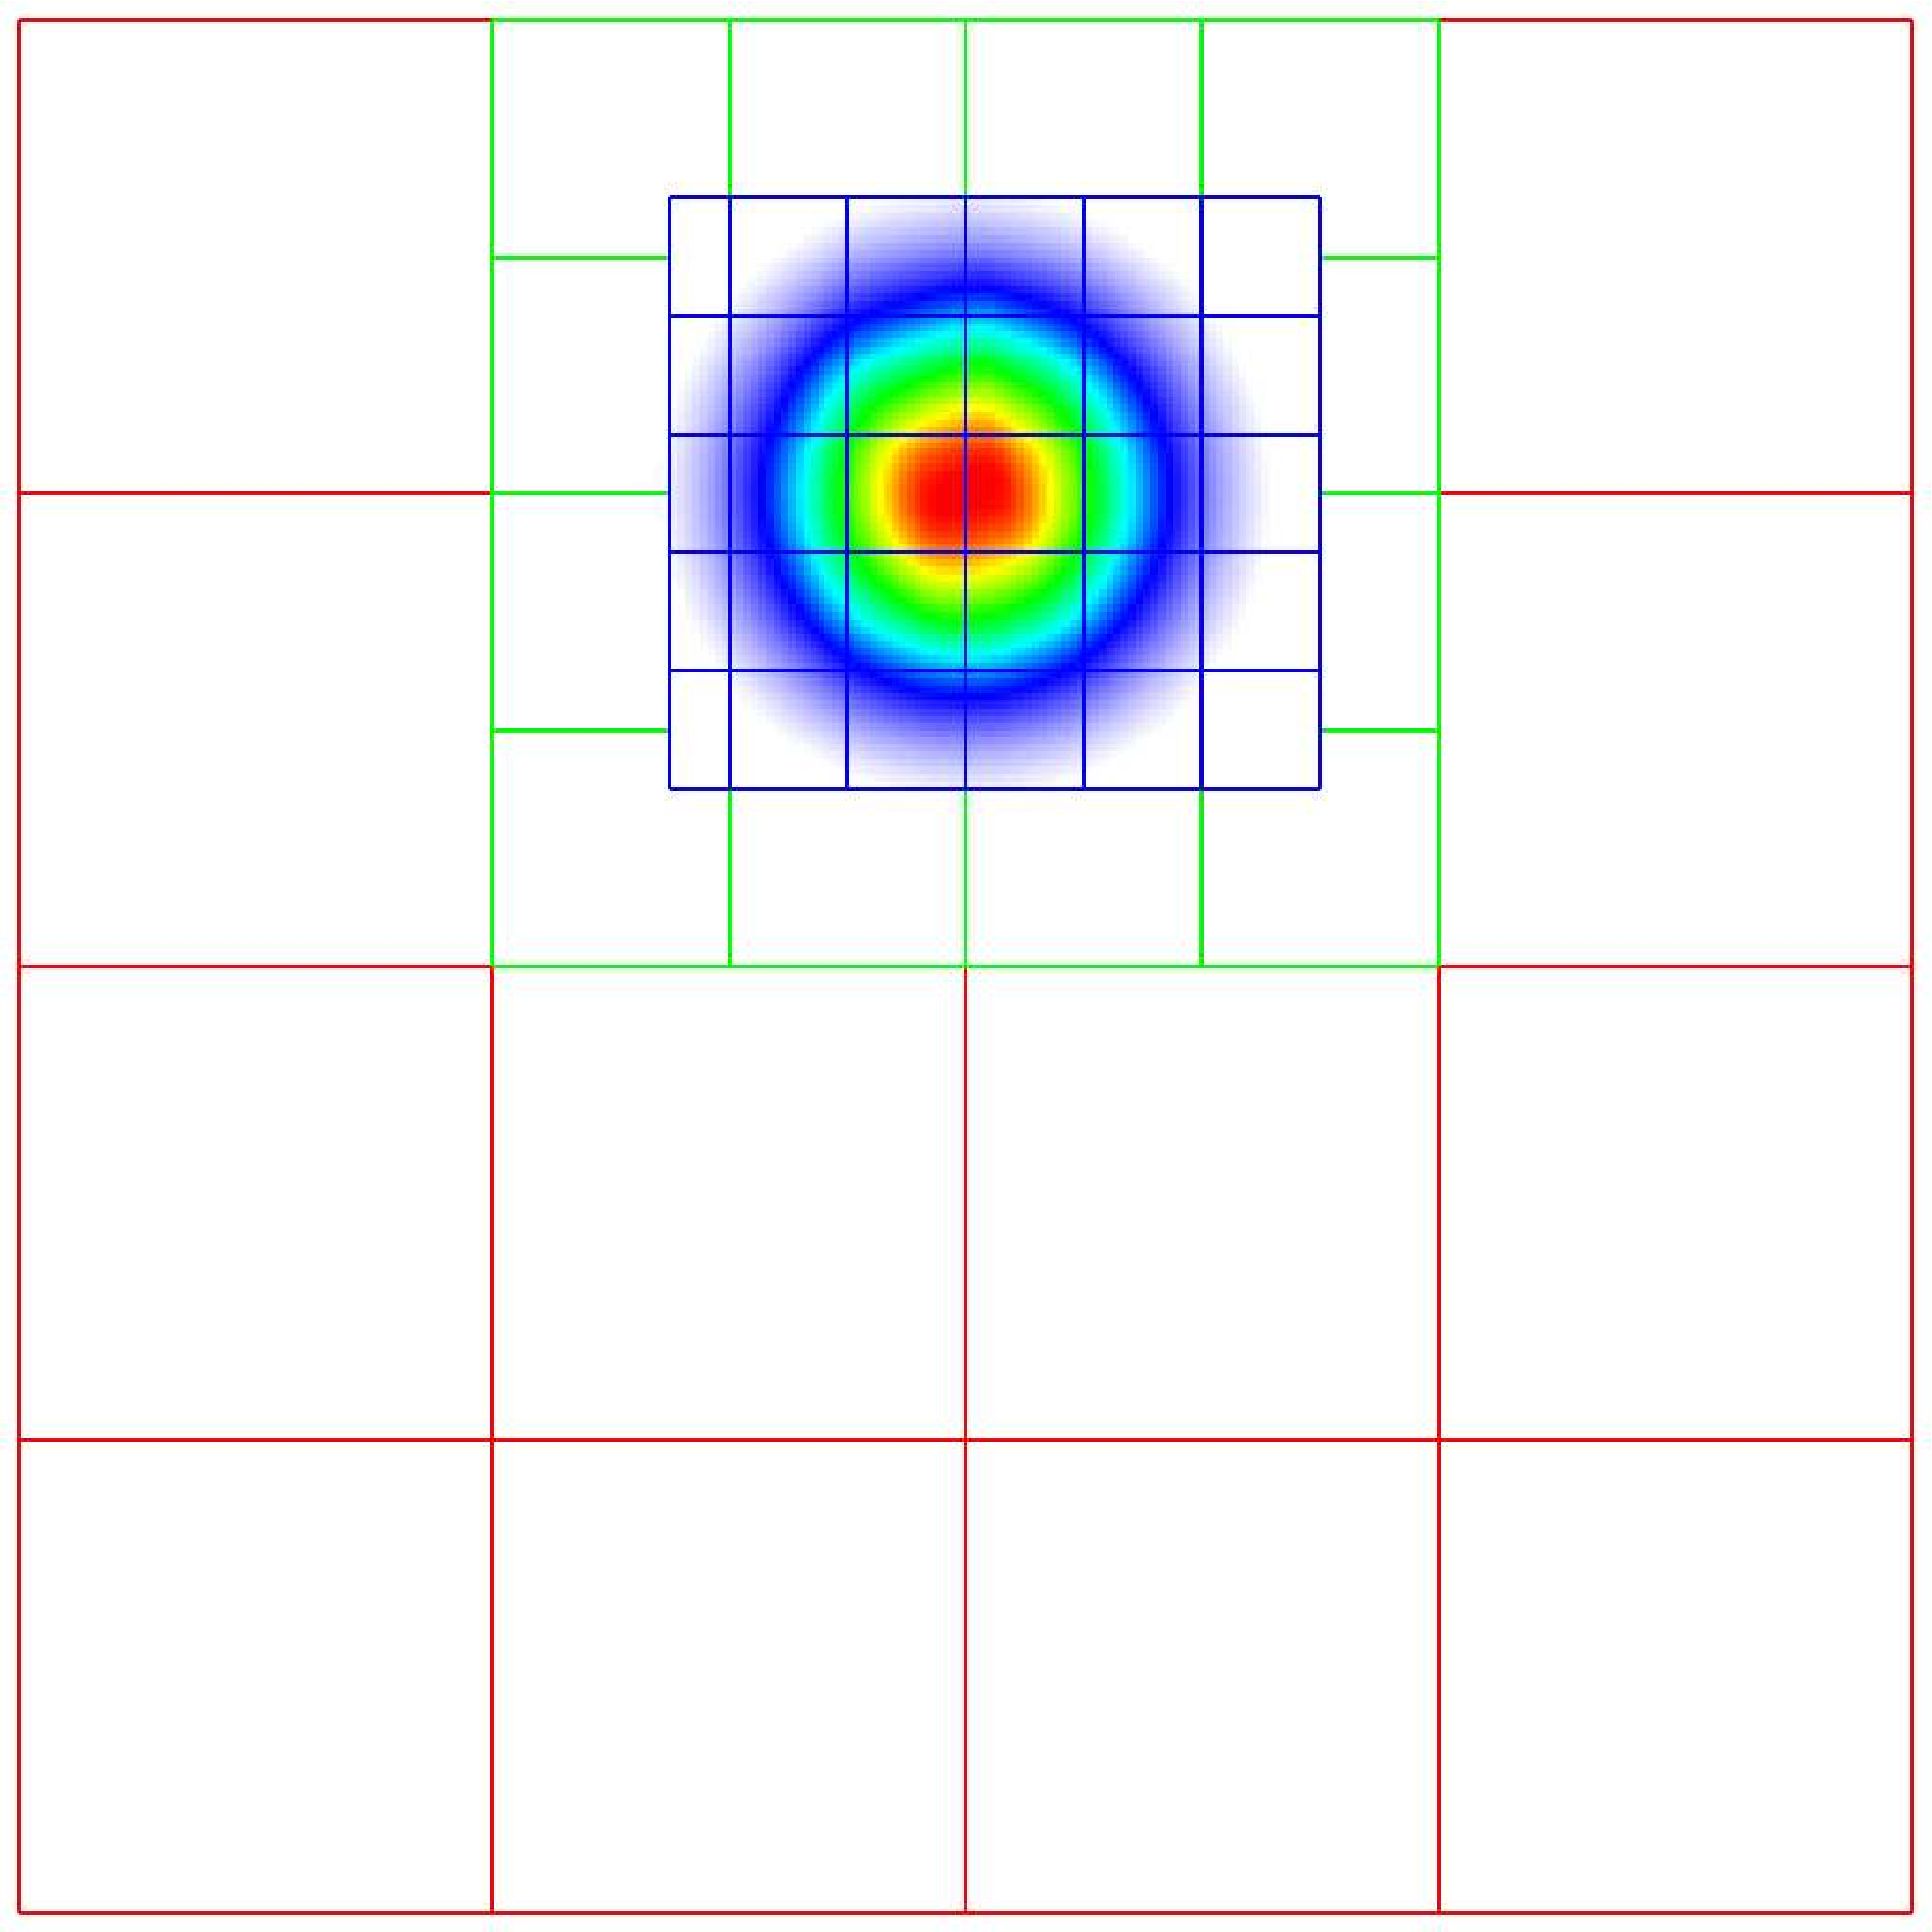
\includegraphics[width=1in]{./AmrCore/figs/Adv5.pdf}
  \caption{\label{fig:Adv} Time sequence ($t=0,0.5,1,1.5,2$~s) of advection of a Gaussian profile using the 
{\tt SingleVortex} tutorial.  The red, green, and blue boxes indicate grids at AMR levels $\ell=0,1$, and $2$.}
\end{figure}

\section{The Advection Equation}
We seek to solve the advection equation on a multi-level, adaptive grid structure:
\begin{equation}
\frac{\partial\phi}{\partial t} = -\nabla\cdot(\phi{\bf U}).
\end{equation}
The velocity field is a specified divergence-free (so the flow field is incompressible)
function of space and time.  The initial scalar field is a
Gaussian profile.  To integrate these equations on a given level, we use a simple conservative update,
\begin{equation}
\frac{\phi_{i,j}^{n+1}-\phi_{i,j}^n}{\Delta t} = \frac{(\phi u)_{i+\myhalf,j}^{n+\myhalf}-(\phi u)_{i-\myhalf,j}^{n+\myhalf}}{\Delta x} + \frac{(\phi v)_{i,j+\myhalf}^{n+\myhalf} - (\phi v)_{i,j-\myhalf}^{n+\myhalf}}{\Delta y},
\end{equation}
where the velocities on faces are prescribed functions of space and time, and the scalars on faces
are computed using a Godunov advection integration scheme.  The fluxes in this case are the face-centered,
time-centered ``$\phi u$'' terms.

We use a subcycling-in-time approach where finer levels are advanced with smaller
time steps than coarser levels, and then synchronization is later performed between levels.
More specifically, the multi-level procedure can most
easily be thought of as a recursive algorithm in which, to advance level $\ell$,
$0\le\ell\le\ell_{\rm max}$, the following steps are taken:
\begin{itemize}
\item Advance level $\ell$ in time by one time step, $\Delta t^{\ell}$, as if it is
the only level.  If $\ell>0$, obtain boundary data (i.e. fill the level $\ell$ ghost cells)
using space- and time-interpolated data from the grids at $\ell-1$ where appropriate.
\item If $\ell<\ell_{\rm max}$
\begin{itemize}
\item Advance level $(\ell+1)$ for $r$ time steps with $\Delta t^{\ell+1} = \frac{1}{r}\Delta t^{\ell}$.
\item Synchronize the data between levels $\ell$ and $\ell+1$.
\end{itemize}
\end{itemize}
Specifically, for a 3-level simulation, depicted graphically in Figure \ref{fig:subcycling}:
\begin{enumerate}
\item Integrate $\ell=0$ over $\Delta t$.
\item Integrate $\ell=1$ over $\Delta t/2$.
\item Integrate $\ell=2$ over $\Delta t/4$.
\item Integrate $\ell=2$ over $\Delta t/4$.
\item Synchronize levels $\ell=1,2$.
\item Integrate $\ell=1$ over $\Delta t/2$.
\item Integrate $\ell=2$ over $\Delta t/4$.
\item Integrate $\ell=2$ over $\Delta t/4$.
\item Synchronize levels $\ell=1,2$.
\item Synchronize levels $\ell=0,1$.
\end{enumerate}
%%%%%%%%%%%%%%%%%%%%%%%%%%%%%
\begin{figure}[htb]
\begin{center}
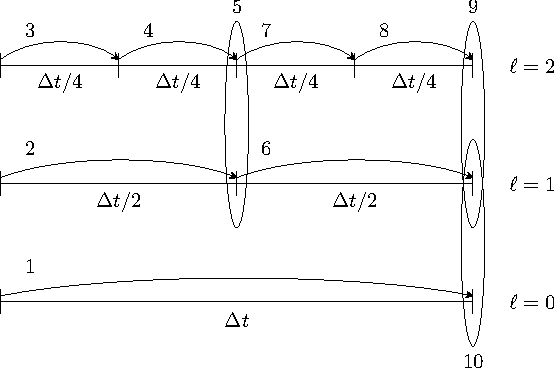
\includegraphics[width=4in]{./AmrCore/figs/subcycling.pdf}
\caption{\label{fig:subcycling} Schematic of subcycling-in-time algorithm.}
\end{center}
\end{figure}
%%%%%%%%%%%%%%%%%%%%%%%%%%%%%
For the scalar field, we keep track volume and time-weighted fluxes at coarse-fine interfaces.

The idea behind the level $\ell/(\ell+1)$ synchronization step is to correct for sources of mismatch in the composite solution:
\begin{enumerate}
\item The data at level $\ell$ that underlie the level  $\ell+1$ data are not synchronized with the level $\ell+1$ data.
This is simply corrected by overwriting covered coarse cells to be the average of the overlying fine cells.
\item The fluxes from the level $\ell$ faces and the level $\ell+1$ faces
do not agree at the $\ell/(\ell+1)$ interface, resulting in a loss of conservation.  
The remedy is to modify the solution in the coarse cells immediately next to the coarse-fine interface
to account for the mismatch stored in the flux register (computed by taking the coarse-level divergence of the
flux register data).
\end{enumerate}






\section{{\tt AmrMesh} and {\tt AmrCore}}

For single-level simulations
(see e.g., {\tt amrex/Tutorials/Basic/HeatEquation\_EX1\_C/main.cpp})
the user needs to build {\tt Geometry}, {\tt DistributionMapping},
and {\tt BoxArray} objects associated with the simulation.  For simulations
with multiple levels of refinement, the {\tt AmrMesh} class can be thought
of as a container to store arrays of these objects (one for each level), and
information about the current grid structure.  The protected data
members of the {\tt AmrMesh} class are:
\begin{lstlisting}[language=cpp]
protected:
    int            verbose;
    int            max_level;       // Maximum allowed level.
    Array<IntVect> ref_ratio;       // Refinement ratios [0:finest_level-1]

    int            finest_level;    // Current finest level.

    Array<int>     n_error_buf;     // Buffer cells around each tagged cell.
    Array<int>     blocking_factor; // Blocking factor in grid generation 
                                    // (by level).
    Array<int>     max_grid_size;   // Maximum allowable grid size (by level).
    Real           grid_eff;        // Grid efficiency.
    int            n_proper;        // # cells required for proper nesting.

    bool use_fixed_coarse_grids;
    int  use_fixed_upto_level;
    bool refine_grid_layout;        // chop up grids to have the number of 
                                    // grids no less the number of procs

    Array<Geometry>            geom;
    Array<DistributionMapping> dmap;
    Array<BoxArray>            grids;    
\end{lstlisting}

{\tt AmrCore.cpp/H} contains the class {\tt AmrCore}, which is derived from
the {\tt AmrMesh} class.

\section{{\tt Cluster}, {\tt ErrorList}, and {\tt TagBox}}

\section{{\tt Interpolater}}

{\tt AMReX\_Interpolater.cpp/H} contains the virtual base class {\tt Interpolater}, which provides
an interface for coarse-to-fine spatial interpolation operators.  Within {\tt AMReX\_Interpolater.cpp/H}
are the derived classes:
\begin{itemize}
\item {\tt NodeBilinear}
\item {\tt CellBilinear}
\item {\tt CellConservativeLinear}
\item {\tt CellConservativeProtected}
\item {\tt CellQuadratic}
\item {\tt PCInterp}
\item {\tt CellConservativeQuartic}
\end{itemize}
The fortran routines that perform the actual work associated with {\tt Interpolater} are 
contained in the files {\tt AMReX\_INTERP\_F.H} and {\tt AMReX\_INTERP\_xD.F}.

\section{{\tt FillPatchUtil}}
{\tt AMReX\_FillPatchUtil.cpp/H} contains as assortment of functions to check for proper nesting
and to help with interpolation.

\section{{\tt FluxRegister}}

{\tt AMReX\_FluxRegister.cpp/H} contains the class {\tt FluxRegister}, which is derived from
the class {\tt BndryRegister} (in {\tt Src/Boundary/AMReX\_BndryRegister}).
In the most general terms, a {\tt FluxRegister} is a special type of {\tt BndryRegister} that
stores and manipulates fluxes at coarse-fine interfaces.
A simple usage scenario comes from a conservative discretization of a hyperbolic system:
\begin{equation}
\frac{\partial\phi}{\partial t} = \nabla\cdot{\bf F}
\rightarrow
\frac{\phi_{i,j}^{n+1}-\phi_{i,j}^n}{\Delta t} = \frac{F_{i+\myhalf,j}-F_{i-\myhalf,j}}{\Delta x} + \frac{F_{i,j+\myhalf} - F_{i,j-\myhalf}}{\Delta y}.
\end{equation}
Consider a two-level, two-dimensional simulation.  A standard methdology for advancing the solution in 
time is to first advance the coarse grid solution ignoring the fine level, and then advance the fine 
grid solution using the coarse level only to supply boundary conditions.  At the coarse-fine interface, 
the area weighted fluxes from the fine grid advance do not in general match the underlying flux from 
the coarse grid face, resulting in a lack of conservation.  Note that for subcycling-in-time algorithms
(where for each coarse grid advance, the fine grid is advanced $r$ times using a coarse grid time step 
reduced by a factor of $r$, where $r$ is the refinement ratio), the coarse grid flux must 
be compared to the area {\it and} time-weighted fine grid fluxes.  A {\tt FluxRegister} accumulates 
and ultimately stores the net difference in fluxes between the coarse grid and fine grid advance over 
each face over a given coarse time step.  The simplest possible synchronization step is to modify
the coarse grid solution in coarse cells immediately adjacent to the coarse-fine interface are updated
to account for the mismatch stored in the {\tt FluxRegister}.

The fortran routines that perform the actual work associated with {\tt FluxRegister} are 
contained in the files {\tt AMReX\_FLUXREG\_F.H} and {\tt AMReX\_FLUXREG\_xD.F}.

\section{{\tt AmrParticles} and {\tt AmrParGDB}}

The {\tt AmrCore/} directory contains derived class for dealing with particles 
in a multi-level framework.  The description of the base classes
are given in Chapter \ref{Chap:Particles}.

{\tt AMReX\_AmrParticles.cpp/H} contains the classes {\tt AmrParticleContainer}
and {\tt AmrTracerParticleContainer}, which are derived from the classes
{\tt ParticleContainer} (in {\tt Src/Particle/AMReX\_Particles})
and {\tt TracerParticleContainer} (in {\tt Src/Particle/AMReX\_TracerParticles}).

{\tt AMReX\_AmrParGDB.cpp/H} contains the class {\tt AmrParGDB}, which is derived from
the class {\tt ParGDBBase} (in {\tt Src/Particle/AMReX\_ParGDB}).


\chapter{{\tt Amr} Source Code}\label{Chap:AmrLevel}
The source code in {\tt amrex\_Src/Amr} contains a number of classes, most notably
the {\tt Amr} class and the {\tt AmrLevel} class.
The {\tt Amr} class is derived from {\tt AmrCore}, and manages data across the 
entire AMR hierarchy of grids.
The {\tt AmrLevel} class is a pure virtual class for managing data at a
single level of refinement.

Many of our mature application codes contain derived classes that inherit directly
from {\tt AmrLevel}.  These include our compressible astrophysics code,
{\tt CASTRO}, and our computational cosmology code, {\tt NYX}.  We also have
NYX for computational cosmology)   We also have 
a pure virtual class called {\tt NavierStokesBase} that inherits from {\tt AmrLevel}
(available in the {\tt AMReX-codes/IAMR} github repository).  Our incompressible
Navier-Stokes code, {\tt IAMR}, as well as our low Mach number combustion code,
{\tt PeleLM}, inherit from {\tt NavierStokesBase}.

The tutorial code in {\tt amrex/Tutorials/Amr/Advection\_AmrLevel} gives a simple
example of a class derived from {\tt AmrLevel} that can be used to solve
the advection equation on a subcycling-in-time AMR hierarchy.  Note that example
is essentially the same as the {\tt amrex/Tutorials/Amr/Advection\_AmrCore} tutorial
and documentation in Chatper \ref{Chap:AmrCore}, except now we use the provided
libraries in {\tt Src/Amr}.

The most important data managed by the {\tt AmrLevel} is an array of {\tt StateData},
which holds the scalar fields, etc., in the boxes that together make up the level.

\section{{\tt StateData}}
{\tt StateData} is a class that essentially holds a pair of {\tt MultiFab}s: one at the old time and one
at the new time. {\tt AMReX} knows how to interpolate in time between these states to get data at
any intermediate point in time. The main data that we care about in our applications codes 
(such as the fluid state) will be stored as {\tt StateData}. Essentially, data is made {\tt StateData}
if we need it to be stored in checkpoints / plotfiles, and/or we want it to be automatically
interpolated when we refine.
An {\tt AmrLevel} stores an array of {\tt StateData} (in a C ++ array called state). We index this array
using integer keys (defined via an enum in, e.g., {\tt AmrLevelAdv.H}):
\begin{lstlisting}[language=cpp]
enum StateType { Phi_Type = 0,
                 NUM_STATE_TYPE };
\end{lstlisting}
In our tutorial code, we use the function {\tt AmrLevelAdv::variableSetup} to tell our simulation about
the {\tt StateData} (e.g., how many variables, ghost cells, nodality, etc.)
Note that if you have more than one {\tt StateType}, each of the different {\tt StateData} 
carried in the state array can have different numbers
of components, ghost cells, boundary conditions, etc. This is the main reason we separate all this
data into separate {\tt StateData} objects collected together in an indexable array.


\chapter{Particles}\label{Chap:Particles}
In addition to the tools for working with mesh data described in previous chapters, $\tt{AMReX}$ provides data structures and iterators for performing data-parallel particle simulations. 
Our approach is particularly suited to particles that interact with data defined on a (possibly adaptive) block-structured hierarchy of meshes. Example use cases include Particle-in-Cell
simulations, Lagrangian tracers, or particles that exert a drag force onto a fluid, such as in multi-phase flow calculations. The overall goals of $\tt{AMReX}$'s particle 
tools are to allow users flexibility in specifying how the particle data is laid out in memory and to handle the parallel communication of particle data automatically.
In the following sections, we give an overview of $\tt{AMReX}$'s particle classes and how to use them.

\section{The Particle}
\label{sec:Particles:Particle}

The particle classes can be used by including the header $\tt{AMReX\_Particles.H}$. The most basic particle data structure is the particle struct itself: 

\begin{lstlisting}[language=cpp]
  Particle<3, 2> p;
\end{lstlisting}

This is a templated data type, designed to allow users flexibility in specifying the number and type of variables that the particles carry. The first template parameter is
the number of extra $\tt{Real}$ variables this particle will have (either single or double precision), while the second is the number of extra integer variables. It is imporant to note
that this is the number of $\emph{extra}$ real and integer variables; a particle will always have at least $\tt{BL\_SPACEDIM}$ $\tt{Real}$ components that store the particle's position
and $\tt{2}$ integer components that store the particle's $\tt{id}$ and $\tt{cpu}$ numbers.
\footnote{Note that $\tt{cpu}$ stores the number of the process the particle was $\emph{generated}$
on, not the one its currently assigned to. This number is set on initialization and never changes, just like the particle $\tt{id}$. In essence, the particles have two integer id numbers, and only the combination of the two is unique. This was done to facilitate the creation of particle initial conditions in parallel.}

The particle struct is designed to store these variables in a way that minimizes padding, which in practice means that the $\tt{Real}$ components always come first, and the integer
components second. Additionally, the required particle variables are stored before the optional ones, for both the real and the integer components. For example, say we want to define
a particle type that stores a mass, three velocity components, and two extra integer flags. Our particle struct would be set up like:

\begin{lstlisting}[language=cpp]
  Particle<4, 2> p;
\end{lstlisting}

and the order of the particle components in would be: x y z m vx vy vz id cpu flag1 flag2. \footnote{Note that for the extra particle components, which component refers to which
variable is an application-specific convention - the particles have 4 extra real comps, but which one is ``mass'' is up to the user. We suggest using an \tt{enum} to keep these indices straight; please see Section~\ref{sec:Particles:Initializing} below for an example of this.} 

\subsection{Setting Particle data}

The $\tt{Particle}$ struct provides a number of methods for getting and setting a particle's data. For the required particle components, there are special, named methods. For the 
``extra'' real and integer data, you can use the $\tt{rdata}$ and $\tt{idata}$ methods, respectively. 

\begin{lstlisting}[language=cpp]
  Particle<2, 2> p;

  p.pos(0) = 1.0;
  p.pos(1) = 2.0;
  p.pos(2) = 3.0;
  p.id() = 1;
  p.cpu()  = 0;

  // p.rdata(0) is the first extra real component, not the 
  // first real component overall
  p.rdata(0) = 5.0;
  p.rdata(1) = 5.0;

  // and likewise for p.idata(0);
  p.rdata(0) = 17;
  p.idata(1) = -64;  
\end{lstlisting}

\section{The ParticleContainer}
\label{sec:Particles:ParticleContainer}
 
One particle by itself is not very useful. To do real calculations, a collection of particles needs to be defined, and the location of the particles within the AMR hierarchy
(and the corresponding MPI process) needs to be tracked as the particle positions change. To do this, we provide the $\tt{ParticleContainer}$ class:

\begin{lstlisting}[language=cpp]
  ParticleContainer<3, 2, 4, 4> mypc;
\end{lstlisting}
   
\subsection{Arrays-of-Structs and Structs-of-Arrays}

Like the $\tt{Particle}$ class itself, the $\tt{ParticleContainer}$ class is templated. The first two template parameters have the same meaning as before: they define the number of each type of variables that the particles in this container will store. In addition, there are two more optional template parameters that allow the user to specify additional particle
variables that will be stored in Struct-of-Array form. The difference between Array-of-Struct and Struct-of-Array data is in how the data is laid
out in memory. For the Array-of-Struct data, all the variables associated with particle 1 are next to each other in memory, followed by all the variables associated with particle
2, and so on. For variables stored in Struct-of-Array style, all the particle data for a given component is next to each other in memory, and each component is stored in a seperate
array. For convenience, we (arbitrarily) refer to the components in the particle struct as particle $\emph{data}$, and components stored in the Struct-of-Arrays as particle
$\emph{attributes}$. See Figure XXX for an illustration.

To see why the distinction between Array-of-Struct and Struct-of-Array data is important, consider the following extreme case. Say you have particles that carry 100 different components,
but that most of the time, you only need to do calculations involving 3 of them (say, the particle positions) at once. In this case, storing all 100 particle variables in the particle
struct is clearly inefficient, since most of the time you are reading 97 extra variables into cache that you will never use. By splitting up the particle variables into stuff that gets 
used all the time (stored in the Array-of-Structs) and stuff that only gets used infrequently (stored in the Struct-of-Arrays), you can in principle acheive much better cache reuse. Of course, the usage pattern of your application likely won't be so clear-cut. Flexibility in how the particle data is stored also makes it easier to interface between $\tt{AMReX}$ and already-existing Fortran subroutines.

Note that while ``extra'' particle data can be stored in either Struct-of-Array or Array-of-Struct style, the particle positions and id numbers are $\emph{always}$ stored in the particle
structs. This is because these particle variables are special and used internally by $\tt{AMReX}$ to assign the particles to grids and to mark particles as valid or invalid, respectively.

\subsection{Constructing ParticleContainers}

A particle container is always associated with a particular set of AMR grids and a particular set of $\tt{DistributionMap}$s that describes which MPI processes those grids live on.
For example, if you only have one level, you can define a $\tt{ParticleContainer}$ to store particles on that level using the following constructor:

\begin{lstlisting}[language=cpp]
    ParticleContainer (const Geometry            & geom,
                       const DistributionMapping & dmap,
                       const BoxArray            & ba);
\end{lstlisting}

Or, if you have multiple levels, you can use following constructor instead:

\begin{lstlisting}[language=cpp]
    ParticleContainer (const Array<Geometry>            & geom,
                       const Array<DistributionMapping> & dmap,
                       const Array<BoxArray>            & ba,
                       const Array<int>                 & rr);
\end{lstlisting}

Note the set of grids used to define the $\tt{ParticleContainer}$ doesn't have to be the same set used to define the simulation's mesh data. However, it is often desirable to have
the two hierarchies track each other. If you are using an $\tt{AmrCore}$ class in your simulation (see Chapter~\ref{Chap:AmrCore}), you can achieve this by using 
the $\tt{AmrParticleContainer}$ class. The constructor for this class takes a pointer to your $\tt{AmrCore}$ derived class, instead:

\begin{lstlisting}[language=cpp]
  AmrTracerParticleContainer (AmrCore* amr_core);
\end{lstlisting}

In this case, the $\tt{Array<BoxArray>}$ and $\tt{Array<DistributionMap>}$ used by your $\tt{ParticleContainer}$ will be updated automatically to match those in
your $\tt{AmrCore}$. 

The $\tt{ParticleContainer}$ stores the particle data in a manner prescribed by the set of AMR grids used to define it. If tiling is turned off, then every grid has its own 
Array-of-Structs and Struct-of-Arrays. Which AMR grid a particle is assigned to is determined by examining its position and binning it, using the domain left edge as an offset. 
By default, a particle is assigned to the finest level that contains its position, although this behavior can be tweaked (see Section~\ref{sec:Particles:Subcycling} below). 
When tiling is enabled, then each $\emph{tile}$ gets its own Struct-of-Arrays and Array-of-Structs instead. Note that this is different than what happens with mesh data. With mesh
data, the tiling is strictly logical; the data is laid out in memory the same whether tiling is turned on or off. With particle data, however, the particles are actually stored in 
a different arrays when tiling is enabled. As with mesh data, the particle tile size can be tuned so that an entire tile's worth of particles will fit into a cache line at once.

Once the particles move, their data may no longer be in the right place in the container. They can be reassigned by calling the $\tt{Redistribute()}$ method of $\tt{ParticleContainer}$.
After calling this method, all the particle will be moved to their proper places in the container, and all invalid particles (particles with id set to $-1$) will be removed. All the 
MPI communication needed to this happens automatically; their is no need for application developers to worry about communicating particle data themselves.

As you build your application, you will likely want to create your own derived $\tt{ParticleContainer}$ class that specializes the template parameters and adds additional 
functionality, like setting the particle initial conditions, moving the particles, etc. See Section~\ref{sec:Particles:Initializing} for an example.

\section{Initializing Particle Data}
\label{sec:Particles:Initializing}

In the following code snippet, we create a derived particle container with 2 real components and 2 integer components, both stored in the Struct-of-Arrays.
We give our derived class an $\tt{InitParticles}$ method that creates one particle per cell on the coarse level, and shows how to set the particle attributes
and add them to the proper container. 

\begin{lstlisting}[language=cpp]

  // These enums are used to keep track of what index means what
  // for the real... 
  struct RealIdx {
    enum {
      eggs = 0,
      ham,
      nattribs
    };
  };
  
  // ... and the integer attributes.
  struct IntIdx {
    enum {
      foo = 0,
      bar,
      nattribs
    };
  };

  // Now we define our ParticleContainer subclass, 
  // passing in the appropriate template parameters.
  class MyParticleContainer
  : public ParticleContainer<0, 0,
                             RealIdx::nattribs,
                             IntIdx::nattribs>
  {
    public:
    
    MyParticleContainer (const Array<Geometry>            & geom,
                         const Array<DistributionMapping> & dmap,
                         const Array<BoxArray>            & ba,
                         const Array<int>                 & rr)
        : ParticleContainer<0, 0,
                            RealIdx::nattribs,
                            IntIdx::nattribs> (geom, dmap, ba, rr) {}

    void InitParticles() {
        const int lev = 0;
        const Geometry& geom = Geom(lev);
        const Real* dx  = geom.CellSize();

        ParticleType p;
        for (MFIter mfi = MakeMFIter(lev); mfi.isValid(); ++mfi) {
            const Box& tile_box = mfi.tilebox();
            const RealBox tile_real_box { tile_box, dx, geom.ProbLo() };

            const int grid_id = mfi.index();
            const int tile_id = mfi.LocalTileIndex();
            auto& particle_tile = GetParticles(lev)[std::make_pair(grid_id, 
                                                                   tile_id)];

            const auto& boxlo = tile_box.smallEnd();
            for (IntVect iv = tile_box.smallEnd(); iv <= tile_box.bigEnd(); 
                 tile_box.next(iv)) {

                // set the particle id and cpu (in the particle struct)
                p.id() = ParticleType::NextID();
                p.cpu() = ParallelDescriptor::MyProc();

                // set the particle positions (also in the struct)
                AMREX_D_TERM(
                p.pos(0) = tile_real_box.lo(0) + (iv[0]- boxlo[0] + 0.5)*dx[0];,
                p.pos(1) = tile_real_box.lo(1) + (iv[1]- boxlo[1] + 0.5)*dx[1];,
                p.pos(2) = tile_real_box.lo(2) + (iv[2]- boxlo[2] + 0.5)*dx[2];
                );

                // set this particle's real attributes
                // (Probably want to do something more 
                // interesting here... )
                std::array<double, RealIdx::nattribs> real_attribs;
                real_attribs[RealIdx::ham]  = 7.0;
                real_attribs[RealIdx::eggs] = 9.0;

                // set this particle's integer attributes (ditto)
                std::array<int, IntIdx::nattribs> int_attribs;
                int_attribs[IntIdx::foo]  = -1;
                int_attribs[IntIdx::bar]  = 12; 

                particle_tile.push_back(p);
                particle_tile.push_back_real(real_attribs);
                particle_tile.push_back_int(int_attribs);
            }
        }
    }
};

\end{lstlisting}

In the above code, because each process only generates particles in grids that it owns, the particles are already in the right place in the container. 
In general, however, users may need to call $\tt{Redistribute()}$ after adding particles, if the processes generate particles they don't own (for example,
if the particle positions are perturbed from the cell centers and thus end up outside their parent grid).

\section{Iterating over Particles}
\label{sec:Particles:Iterating}

To iterate over the particles on a given level in your container, you can use the $\tt{ParIter}$ class, which comes in 
both const and non-const flavors. For example:

\begin{lstlisting}[language=cpp]

for (MyParIter pti(*this, lev); pti.isValid(); ++pti) {
    auto& particles = pti.GetArrayOfStructs();
    for (unsigned i = 0; i < pti.numParticles(); ++i) {
        const ParticleType& p = particles[i];
        // do stuff with p...
    }
}
\end{lstlisting}

The outer loop will execute once every grid (or tile, if tiling is enabled) \emph{that contains particles}; grids or tiles
that don't have any particles will be skipped. 

\section{Passing particle data into Fortran routines}
\label{sec:Particles:Fortran}

Because the $\tt{AMReX}$ particle struct is a Plain-Old-Data type, it is interoperable with FORTRAN when the $\tt{bind(C)}$
attribute is used. It is therefore possible to pass a grid or tile worth of particles into fortran routines for processing,
instead of iterating over them in C++. You can also define a Fortran derived type that is equivalent to C struct used for the
particles. For example:

\begin{lstlisting}[language=fortran]

    use amrex_fort_module, only: amrex_real
    use iso_c_binding ,    only: c_int

    type, bind(C)  :: particle_t
       real(amrex_real) :: pos(3)
       real(amrex_real) :: vel(3)
       real(amrex_real) :: acc(3)
       integer(c_int)   :: id
       integer(c_int)   :: cpu
    end type particle_t

\end{lstlisting}

is equivalent to particle struct you get with $\tt{Particle<6, 0>}$.

\section{Interacting with Mesh Data}
\label{sec:Particles:Interacting}

SumBoundary. Syncing across levels. ElectrostaticPIC tutorial.

\section{Short Range Forces}
\label{sec:Particles:ShortRange}

Neighbor particles. Optional communication. The ShortRangeParticles tutorial.

\section{Particle IO}
\label{sec:Particles:IO}

IO Routines (ASCII and binary), visualization options. Converter python script.

\section{Subcycling with Particles}
\label{sec:Particles:Subcycling}

This is hard. Ghosts and Virtuals.  



\chapter{Fortran Interface}\label{Chap:Fortran}
The core of \amrex\ is written in \cpp.  For Fortran users who want to
write all of their programs in Fortran, \amrex\ provides Fortran
interfaces around most of functionalities except for 
the {\tt AmrLevel} class (Chapter~\ref{Chap:AmrLevel}).  
and particles (Chapter~\ref{Chap:Particles}) 
We should not confuse the Fortran
interface in this chapter with the Fortran kernel functions called
inside {\tt MFIter} loops in \cpp codes
(Section~\ref{sec:basics:fortran}).  For the latter, Fortran is used
in some sense as a domain-specific language with native
multi-dimensional arrays, whereas here Fortran is used to drive the
whole application code.  In order to better understand \amrex, Fortran
interface users should read the rest of the User's Guide except for
Chapters~\ref{Chap:AmrLevel} \& \ref{Chap:Particles}. 

\section{Getting Started}

We have discussed \amrex's build systems in
Chapter~\ref{Chap:BuildingAMReX}.  To build with GNU Make, we need to
include the Fortran interface source tree into the make system.  The
source codes for the Fortran interface are in {\tt
amrex/Src/F\_Interfaces} and there are several sub-directories.  The
{\tt Base} directory includes sources for the basic functionality, the
{\tt AmrCore} directory wraps around {\tt AmrCore} class
(Chapter~\ref{Chap:AmrCore}), and the {\tt Octree} adds support for
octree type of AMR grids.  Each directory has a {\tt Make.package}
file that can be included in make files (see {\tt
Tutorials/Basic/HelloWorld\_F} and {\tt Tutorials/Amr/Advection\_F}
for examples).  The {\tt libamrex} approach includes the Fortran
interface by default.  The CMake approach does not support the Fortran
interface yet.

A simple example can be found at {\tt Tutorials/Basic/HelloWorld\_F/}.
The source code is shown below in it entirety.  
\begin{lstlisting}[language=fortran]
subroutine amrex_fmain () bind(c)
  use amrex_base_module
  implicit none
  if (amrex_parallel_ioprocessor()) then
     print *, "Hello world!"
  end if
end subroutine amrex_fmain
\end{lstlisting}
Note that there is no {\tt program main} in the Fortran code.  The
{\tt main} function is actually in {\tt
  Src/F\_Interfaces/Base/AMReX\_fi\_main.cpp}.  That {\tt main}
function initializes and finalizes \amrex, and calls {\tt amrex\_fmain}
function in between.

To access \amrex\ Fortran interfaces, we can use these three
modules, {\tt amrex\_base\_module} for the basics functionalities
(Section~\ref{sec:fi:basics}), {\tt amrex\_amrcore\_module} for AMR
support (Section~\ref{sec:fi:amrcore}) and {\tt amrex\_octree\_module}
for octree style AMR (Section~\ref{sec:fi:octree}).

\section{The Basics}
\label{sec:fi:basics}

Module {\tt amrex\_base\_module} is a collection of various Fortran
modules providing interfaces to most of the basics of \amrex\ \cpp\
library {Chapter~\ref{Chap:Basics}).  These modules shown in this
section can be used without being explicitly included because they are
included by {\tt amrex\_base\_module}.

The spatial dimension is an integer parameter {\tt amrex\_spacedim}.
We can also use the {\tt AMREX\_SPACEDIM} macro in preprocessed
Fortran codes (e.g., {\tt .F90} files) just like in the \cpp\
codes.  Unlike in \cpp, the convention for \amrex\ Fortran interface
is coordinate direction index starts with 1.

There is an integer parameter {\tt amrex\_real}, a Fortran
kind parameter for {\tt real}.  Fortran {\tt real(amrex\_real)}
corresponds to {\tt amrex::Real} in \cpp, which is either double or
single precision depending the setting of precision.

Module {\tt amrex\_parallel\_module} ({\tt
  Src/F\_Interfaces/Base/AMReX\_parallel\_mod.F90}) includes wrappers
to the {\tt ParallelDescriptor} namespace, which is in turn a wrapper
to the parallel communication library used by \amrex\ (e.g. MPI).

Module {\tt amrex\_parmparse\_module} ({\tt
  Src/Base/AMReX\_parmparse\_mod.F90}) provides interface to {\tt
  ParmParse} (Section~\ref{sec:basics:parmparse}.  Here are some
examples.
\begin{lstlisting}[language=fortran]
  type(amrex_parmparse) :: pp
  integer :: n_cell, max_grid_size
  call amrex_parmparse_build(pp)
  call pp%get("n_cell", n_cell)
  max_grid_size = 32 ! default size
  call pp%query("max_grid_size", max_grid_size)
  call amrex_parmpase_destroy(pp) ! optional if compiler supports finalization
\end{lstlisting}
Finalization is a Fortran 2003 feature that some compilers may not
support.  For those compilers, we must explicitly destroy the objects,
otherwise there will be memory leaks.  This applies to many other
derived types.

{\tt amrex\_box} is a derived type in {\tt amrex\_box\_module} {\tt
  Src/F\_Interfaces/Base/AMReX\_box\_mod.F90}.  It has three members,
{\tt lo} (lower corner), {\tt hi} (upper corner) and {\tt nodal}
(logical flag for index type).  

{\tt amrex\_geometry} is a wrapper for the {\tt Geometry} class
containing information for the physical domain.  Below is an example
of building it.
\begin{lstlisting}[language=fortran]
  integer :: n_cell
  type(amrex_box) :: domain
  type(amrex_geometry) : geom
  ! n_cell = ...
  ! Define a single box covering the domain
  domain = amrex_box((/0,0,0/), (/n_cell-1, n_cell-1, n_cell-1/))
  ! This defines a amrex_geometry object.
  call amrex_geometry_build(geom, domain)
  !
  ! ...
  !
  call amrex_geometry_destroy(geom)
\end{lstlisting}


{\tt amrex\_boxarray} ({\tt
  Src/F\_Interfaces/Base/AMReX\_boxarray\_mod.F90}) is a wrapper for
the {\tt BoxArray} class, and {\tt amrex\_distromap} ({\tt
  Src/F\_Interfaces/Base/AMReX\_distromap\_mod.F90}) is a wrapper for
the {\tt DistributionMapping} class.  Here is an example of
building a {\tt BoxArray} and a {\tt DistributionMapping}.
\begin{lstlisting}[language=fortran]
  integer :: n_cell
  type(amrex_box) :: domain
  type(amrex_boxarray) : ba
  type(amrex_distromap) :: dm
  ! n_cell = ...
  ! Define a single box covering the domain
  domain = amrex_box((/0,0,0/), (/n_cell-1, n_cell-1, n_cell-1/))
  ! Initialize the boxarray "ba" from the single box "bx"
  call amrex_boxarray_build(ba, domain)
  ! Break up boxarray "ba" into chunks no larger than "max_grid_size"
  call ba%maxSize(max_grid_size)
  ! Build a DistributionMapping for the boxarray
  call amrex_distromap_build(dm, ba)
  !
  ! ...
  !
  call amrex_distromap_distromap(dm)
  call amrex_boxarray_destroy(ba)
\end{lstlisting}

Given {\tt amrex\_boxarray} and {\tt amrex\_distromap}, we can build
{\tt amrex\_multifab}, a wrapper for the {\tt MultiFab} class, as
follows. 
\begin{lstlisting}[language=fortran]
  integer :: ncomp, nghost
  type(amrex_boxarray) : ba
  type(amrex_distromap) :: dm
  type(amrex_multifab) :: mf, ndmf
  ! Build amrex_boxarray and amrex_distromap
  ! ncomp = ...
  ! nghost = ...
  ! ...
  ! Build amrex_multifab with ncomp component and nghost ghost cells
  call amrex_multifab_build(mf, ba, dm, ncomp, nghost)
  ! Build a nodal multifab
  call amrex_multifab_build(ndmf,ba,dm,ncomp,nghost,(/.true.,.true.,.true./))
  !
  ! ...
  !
  call amrex_multifab_destroy(mf)
  call amrex_multifab_destroy(ndmf)
\end{lstlisting}
There are many type-bound procedures for {\tt amrex\_multifab}.  For
example
\begin{lstlisting}[language=fortran]
  ncomp   ! Return the number of components
  nghost  ! Return the number of ghost cells
  setval  ! Set the data to the given value 
  copy    ! Copy data from given amrex_multifab to this amrex_multifab
\end{lstlisting}
Note that the {\tt copy} function here only works on copying data from
another {\tt amrex\_multifab} built with the same {\tt
  amrex\_distromap}, like the {\tt MultiFab::Copy} function in \cpp.
{\tt amrex\_multifab} also has two parallel communication procedures,
{\tt fill\_boundary} and {\tt parallel\_copy}.  Their and interface
and usage are very similar to functions {\tt FillBoundary} and {\tt
  ParallelCopy} for {\tt MultiFab} in \cpp.
\begin{lstlisting}[language=fortran]
  type(amrex_geometry) :: geom
  type(amrex_multifab) :: mf, mfsrc
  ! ...
  call mf%fill_boundary(geom)       ! Fill all components
  call mf%fill_boundary(geom, 1, 3) ! Fill 3 components starting with component 1

  call mf%parallel_copy(mfsrc, geom) ! Parallel copy from another multifab
\end{lstlisting}
It should be emphasized that the component index for {\tt
  amrex\_multifab} starts with 1 following Fortran convention.  This
is different from \cpp\ part of \amrex.

\amrex\ provides a Fortran interface to {\tt MFIter} for iterating
over the data in {\tt amrex\_multifab}.  The Fortran type for this is
{\tt amrex\_mfiter}.  Here is an example of using {\tt amrex\_mfiter}
to loop over {\tt amrex\_multifab} with tiling and launch a kernel
function.
\begin{lstlisting}[language=fortran]
  integer :: plo(4), phi(4)
  type(amrex_box) :: bx
  real(amrex_real), contiguous, dimension(:,:,:,:), pointer :: po, pn
  type(amrex_multifab) :: old_phi, new_phi
  type(amrex_mfiter) :: mfi
  ! Define old_phi and new_phi ...
  ! In this example they are built with the same boxarray and distromap.
  ! And they have the same number of ghost cells and 1 component.
  call amrex_mfiter_build(mfi, old_phi, tiling=.true.)
  do while (mfi%next())
    bx = mfi%tilebox()
    po => old_phi%dataptr(mfi)
    pn => new_phi%dataptr(mfi)
    plo = lbound(po)
    phi = ubound(po)
    call update_phi(bx%lo, bx&hi, po, pn, plo, phi)
  end do
  call amrex_mfiter_destroy(mfi)
\end{lstlisting}
Here procedure {\tt update\_phi} is
\begin{lstlisting}[language=fortran]
 subroutine update_phi (lo, hi, pold, pnew, plo, phi)
  integer, intent(in) :: lo(3), hi(3), plo(3), phi(3)
   real(amrex_real),intent(in   ) pold(plo(1):phi(1),plo(2):phi(2),plo(3):phi(3))
   real(amrex_real),intent(inout) pnew(plo(1):phi(1),plo(2):phi(2),plo(3):phi(3))
   ! ...
 end subroutine update_phi
\end{lstlisting}
Note that {\tt amrex\multifab}'s procedure {\tt dataptr} takes {\tt
  amrex\_mfiter} and returns a 4-dimensional Fortran pointer.  For
performance, we should declare the pointer as {\tt contiguous}.  In
\cpp, the similar operation returns a reference to {\tt FArrayBox}.
However, {\tt FArrayBox} and Fortran pointer have a similar capability
of containing array bound information.  We can call {\tt lbound} and
{\tt ubound} on the pointer to return its lower and upper bounds.  The
first three dimensions of the bounds are spatial and the fourth is for
the number of component.

Many of the derived Fortran types in \amrex\ (e.g., {\tt
  amrex\_multifab}, {\tt amrex\_boxarray}, {\tt amrex\_distromap},
{\tt amrex\_mfiter}, and {\tt amrex\_geometry}) contain a {\tt
  type(c\_ptr)} that points a \cpp\ object.  They also contain a
logical type indicating whether or not this object owns the underlying
object (i.e., responsible for deleting the object).  Due to the
semantics of Fortran, one should not return these types with
functions.  Instead we should pass them as arguments to procedures
(preferably with {\tt intent} specified).  These five types all have
{\tt assignment(=)} operator that performs a shallow copy.  After the
assignment, the original objects still owns the data and the copy is
just an alias.  For example,
\begin{lstlisting}[language=fortran]
  type(amrex_multifab) :: mf1, mf2
  call amrex_multifab_build(mf1, ...)
  call amrex_multifab_build(mf2, ...)
  ! At this point, both mf1 and mf2 are data owners
  mf2 = mf1   ! This will destroy the original data in mf2.
              ! Then mf2 becomes a shallow copy of mf1.
              ! mf1 is still the owner of the data.
  call amrex_multifab_destroy(mf1)
  ! mf2 no longer contains a valid pointer because mf1 has been destroyed. 
  call amrex_multifab_destroyed(mf2)  ! But we still need to destroy it.
\end{lstlisting}
If we need to transfer the ownership, {\tt amrex\_multifab}, {\tt
  amrex\_boxarray} and {\tt amrex\_distromap} provide type-bound {\tt
  move} procedure.  We can use it as follows
\begin{lstlisting}[language=fortran]
  type(amrex_multifab) :: mf1, mf2
  call amrex_multifab_build(mf1, ...)
  call mf2%move(mf1)   ! mf2 is now the data owner and mf1 is not.
  call amrex_multifab_destroy(mf1)
  call amrex_multifab_destroyed(mf2)
\end{lstlisting}
{\tt amrex\_multifab} also has a type-bound {\tt swap} procedure for
exchanging the data.

\amrex\ also provides {\tt amrex\_plotfile\_module} for writing
plotfiles.  The interface is similar to the \cpp versions.

\section{Amr Core Infrastructure}
\label{sec:fi:amrcore}

Module {\tt amrex\_amr\_module} provides interfaces to AMR core
infrastructure.  With AMR, subroutine {\tt amrex\_fmain} should look
like below,
\begin{lstlisting}[language=fortran]
  subroutine amrex_fmain () bind(c)
    use amrex_amr_module
    implicit none  
    call amrex_amrcore_init()
    call my_amr_init()       ! user's own code, not part of AMReX
    ! ...
    call my_amr_finalize()   ! user's own code, not part of AMReX
    call amrex_amrcore_finalize()
  end subroutine amrex_fmain
\end{lstlisting}
Here we need to call {\tt amrex\_amrcore\_init} and {\tt
  amrex\_amrcore\_finalize}.  And usually we need to call application
code specific procedures to provide some ``hooks'' needed by \amrex.
In \cpp, this is achieved by using virtual functions.  In Fortran, we
need to call
\begin{lstlisting}[language=fortran]
  subroutine amrex_init_virtual_functions (mk_lev_scrtch, mk_lev_crse, &
                                           mk_lev_re, clr_lev, err_est)

    ! Make a new level from scratch using provided boxarray and distromap
    ! Only used during initialization.
    procedure(amrex_make_level_proc)  :: mk_lev_scrtch
    ! Make a new level using provided boxarray and distromap, and fill
    ! with interpolated coarse level data.
    procedure(amrex_make_level_proc)  :: mk_lev_crse
    ! Remake an existing level using provided boxarray and distromap,
    ! and fill with existing fine and coarse data.
    procedure(amrex_make_level_proc)  :: mk_lev_re
    ! Delete level data
    procedure(amrex_clear_level_proc) :: clr_lev
    ! Tag cells for refinement
    procedure(amrex_error_est_proc)   :: err_est
  end subroutine amrex_init_virtual_functions
\end{lstlisting}
We need to provide five functions and these functions have three types
of interfaces:
\begin{lstlisting}[language=fortran]
  subroutine amrex_make_level_proc (lev, time, ba, dm) bind(c)
    import
    implicit none
    integer, intent(in), value :: lev
    real(amrex_real), intent(in), value :: time
    type(c_ptr), intent(in), value :: ba, dm
  end subroutine amrex_make_level_proc
  
  subroutine amrex_clear_level_proc (lev) bind(c)
    import
    implicit none
    integer, intent(in) , value :: lev
  end subroutine amrex_clear_level_proc
  
  subroutine amrex_error_est_proc (lev, tags, time, tagval, clearval) bind(c)
    import
    implicit none
    integer, intent(in), value :: lev
    type(c_ptr), intent(in), value :: tags
    real(amrex_real), intent(in), value :: time
    character(c_char), intent(in), value :: tagval, clearval
  end subroutine amrex_error_est_proc
\end{lstlisting}
{\tt Tutorials/Amr/Advection\_F/Source/my\_amr\_mod.F90} shows an
example of the setup process.  The user provided {\tt
  procedure(amrex\_error\_est\_proc)} has a {\tt tags} argument that
is of type {\tt c\_ptr} and its value is a pointer to a \cpp\ {\tt
  TagBoxArray} object.  We need to convert this into a Fortran {\tt
  amrex\_tagboxarray} object.
\begin{lstlisting}[language=fortran]
  type(amrex_tagboxarray) :: tag
  tag = tags
\end{lstlisting}

Module {\tt amrex\_fillpatch\_module} provides interface to
\cpp\ functions {\tt FillPatchSinglelevel} and {\tt
  FillPatchTwoLevels}.   To use it, the application code needs to
provide procedures for interpolation and filling physical boundaries.
See {\tt Tutorials/Amr/Advection\_F/Source/fillpatch\_mod.F90} for an
example. 

Module {\tt amrex\_fluxregister\_module} provides interface to {\tt
  FluxRegister} (Section~\ref{sec:amrcore:fluxreg}).  Its usage is
demonstrated in the tutorial at {\tt
  Tutorials/Amr/Advection\_F/}. 

\section{Octree}
\label{sec:fi:octree}

In \amrex, the union of fine level grids is properly contained within
the union of coarse level grids.  There are no required direct
parent-child connections between levels.  Therefore, grids in \amrex\
in general cannot be represented by trees.  Nevertheless, octree type
grids are supported via Fortran interface, because \amrex\ grids are
more general than octree grids.  A tutorial example using {\tt
  amrex\_octree\_module} ({\tt
  Src/F\_Interfaces/Octree/AMReX\_octree\_mod.f90}) is available at
{\tt Tutorials/Amr/Advection\_octree\_F/}.  Procedures {\tt
  amrex\_octree\_init} and {\tt amrex\_octree\_finalize} must be
called as follows,
\begin{lstlisting}[language=fortran]
  subroutine amrex_fmain () bind(c)
    use amrex_amrcore_module
    use amrex_octree_module
    implicit none
    call amrex_octree_int()  ! This should be called first.
    call amrex_amrcore_init()
    call my_amr_init()       ! user's own code, not part of AMReX
    ! ...
    call my_amr_finalize()   ! user's own code, not part of AMReX
    call amrex_amrcore_finalize()
    call amrex_octree_finalize()
  end subroutine amrex_fmain
\end{lstlisting}
By default, the grid size is $8^3$, and this can be changed via {\tt
  ParmParse} parameter {\tt amr.max\_grid\_size}.  Module {\tt
  amrex\_octree\_module} provides {\tt amrex\_octree\_iter} that can
be used to iterate over leaves of octree.  For example,
\begin{lstlisting}[language=fortran]
  type(amrex_octree_iter) :: oti
  type(multifab) :: phi_new(*)   ! one multifab for each level
  integer :: ilev, igrd
  type(amrex_box) :: bx
  real(amrex_real), contiguous, pointer, dimension(:,:,:,:) :: pout
  call amrex_octree_iter_build(oti)
  do while(oti%next())
     ilev = oti%level()
     igrd = oti%grid_index()
     bx   = oti%box()
     pout => phi_new(ilev)%dataptr(igrd)
     ! ...
  end do
  call amrex_octree_iter_destroy(oti)
\end{lstlisting}



\chapter{Embedded Boundaries}\label{Chap:EB}
\newcommand{\xbold}{{\bf x}}
\newcommand{\ibold}{{\bf i}}
\newcommand{\jbold}{{\bf j}}
\newcommand{\kbold}{{\bf k}}
\newcommand{\nbold}{{\bf k}}
\newcommand{\cbold}{{\bf k}}
\newcommand{\ebis}{{\tt EBIndexSpace}}
\newcommand{\baseif}{{\tt BaseIF}}
\newcommand{\sphereif}{{\tt SphereIF}}
\newcommand{\transformif}{{\tt TransformIF}}
\newcommand{\latheif}{{\tt LatheIF}}
\newcommand{\unionif}{{\tt UnionIF}}
\newcommand{\intersectionif}{{\tt IntersectionIF}}
\newcommand{\geom}{{\tt GeometryShop}}
\newcommand{\parm}{{\tt ParmParse}}

\section{Overview of Embedded Boundary Description}
\label{sec:EB:EBOverview}

For computations with complex geometries, $\tt{AMReX}$ provides data
structures and algorithms to employ an embedded boundary (EB) approach to
PDE discretizations.    In this approach, the underlying computational
mesh is uniform and block-structured, but the boundary of the irregular-shaped
computational domain conceptually cuts through this mesh.  Each cell in the mesh
becomes labeled as regular, cut or covered, and the finite-volume based
discretization methods traditionally used in AMReX applications can be
modified to incorporate these cell shapes.  See Figure~\ref{fig::ebexample}
for an illustration.
\begin{figure}[h]
  \centering
  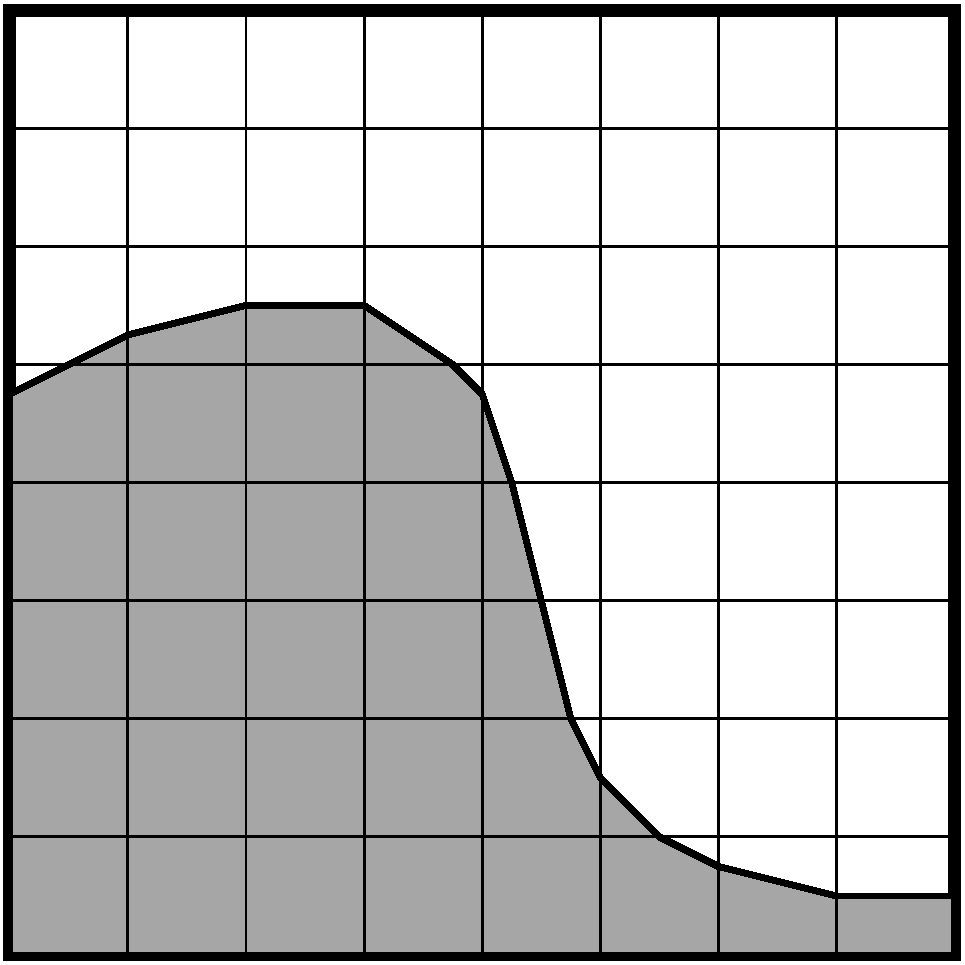
\includegraphics[width=0.25\textwidth]{./EB/EB_example.pdf}
  \caption{\label{fig::ebexample}In the embedded boundary approach to
    discretizing PDEs, the (uniform) rectangular mesh is cut by the
    irregular shape of the computational domain.  The cells in the
    mesh are label as regular, cut or covered.}
\end{figure}
Because this is a relatively simple grid
generation technique, computational meshes for rather complex geometries
can be generated quickly and robustly.  However, the technique 
can produce arbitrarily small cut cells in the domain.  In practice such small
cells can have significant impact on the robustness and stability of
traditional finite volume methods.  In this chapter we overview
a class of approaches to deal with this ``small cell'' problem in a
robust and efficient way, and discuss the tools and data that $\tt{AMReX}$
provides in order to implement them.  

Note that in a completely general implementation of the EB approach, 
there would be no restrictions on the shape or complexity of the EB surface.  
With this generality comes the possibility that the process of "cutting" the cells
results in a single $(i,j,k$) cell being broken into multiple cell fragments.
%In the block-structured context of $\tt{AMReX}$, this would trigger a significant complication
%because the state data (as well as the geometrical and cell
%connectivity information) can no longer be managed using the logically rectangular
%data structures with implied connectivity graphs that are native to the framework.  Because of this,
The current release of $\tt{AMReX}$ does not support multi-valued cells, thus there is a
practical restriction on the complexity of domains (and numerical algorithms) supported.  
AMReX support for EB with AMR will be available by early 2018;
EB support for multi-valued cells will follow.
%as it leads to complexities in data communication patterns
%and inter-level data transfer operations.  
%In both cases however, extended support is
%planned for future releases of the library, and the software infrastructure
%underlying the implementation described in this document have been designed with these
%extensions in mind.

This chapter discusses the EB tools, data structures and algorithms currently supported by
$\tt{AMReX}$ to enable the construction of discretizations of conservation law systems.
The discussion will focus on general requirements associated with building fluxes and
taking divergences of them to advance such systems.  We also give examples of how to
initialize the geometry data structures and access them to build the numerical difference
operators.

\subsection{Finite Volume Discretizations}
Consider a system of PDEs to advance a conserved quantity $U$
with fluxes $F$:
\begin{equation}
\frac{\partial U}{\partial t} + \nabla \cdot F = 0.
\label{eqn::hypsys}
\end{equation}
A conservative, finite volume discretization starts with
the divergence theorm
$$
\int_V \nabla \cdot F dV = \int_{\partial V} F \cdot n dA.
$$
In an embedded boundary cell, the ``conservative divergence'' is discretized  (as
$D^c(F)$) as follows
\begin{equation}
D^c(F) = \frac{1}{\kappa h} \left( \sum^D_{d = 1}
  (F_{d, hi}A_{d,hi} - F_{d, lo}A_{d,lo})  + F^{EB} A^{EB} \right).
\label{eqn::ebdiv}
\end{equation}

Geometry is discretely represented by volumes ($V = \kappa h^d$) and apertures 
($A= \alpha h^{d-1}$), where $h$ is the (uniform) mesh spacing at that AMR level,
$\kappa$ is the volume fraction and $\alpha$ are the area fractions.
Without multivalued cells the volume fractions, area fractions and cell and face centroids 
(see Figure~\ref{fig::volume}) are the only geometric information needed to 
compute second-order fluxes centered at the face centroids,  
and to infer the connectivity of the cells.  
Cells are connected if adjacent on the Cartesian mesh, and only via
coordinate-aligned faces on the mesh.  If an aperture, $\alpha = 0$, between two
cells, they are not directly connected to each other.

\begin{figure}[h]
  \centering
  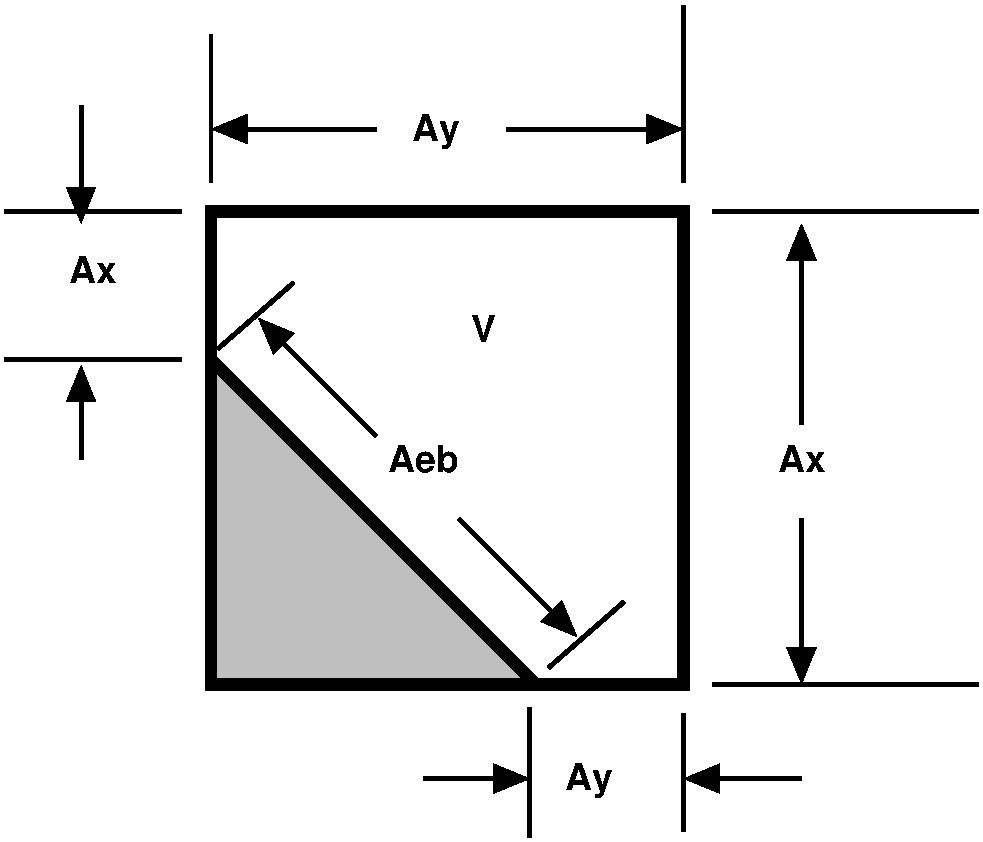
\includegraphics[width=0.25\textwidth]{./EB/areas_and_volumes.pdf}
  \hspace{1in} 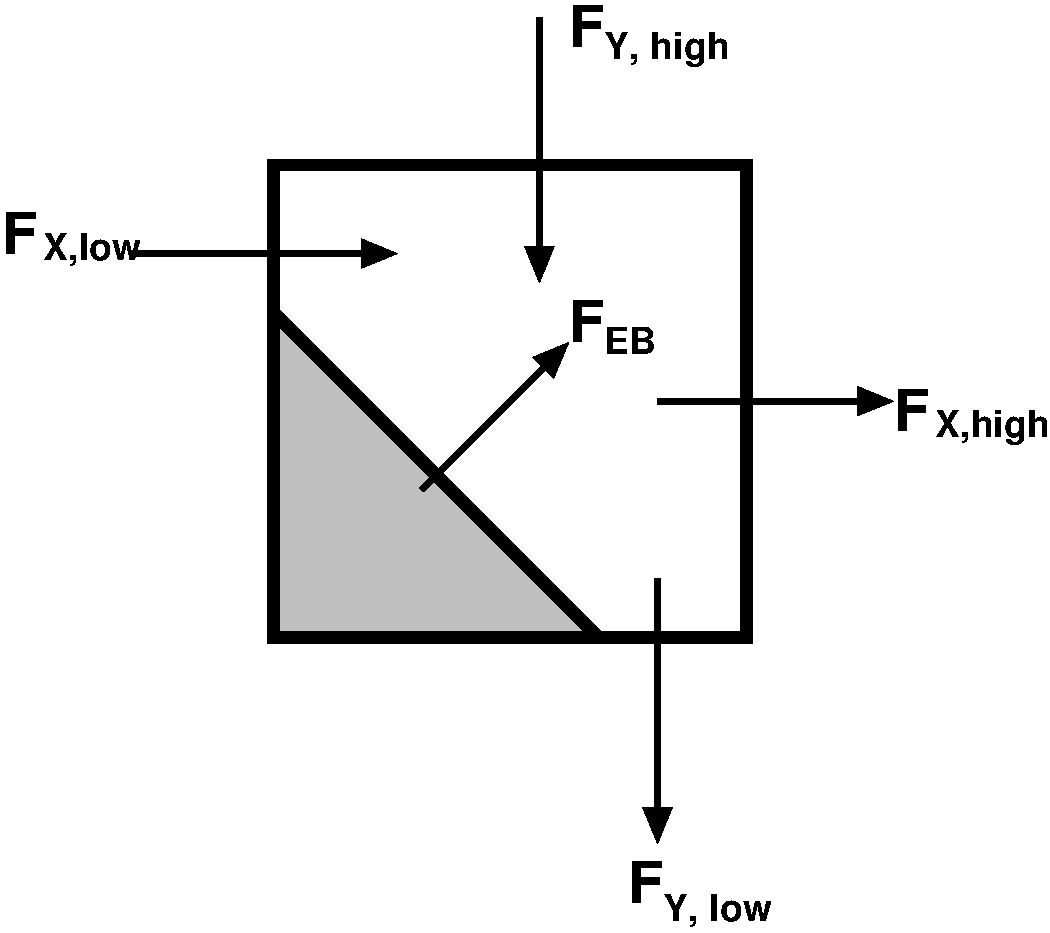
\includegraphics[width=0.25\textwidth]{./EB/eb_fluxes.pdf}
  \caption{\label{fig::volume} (a) A typical two-dimensional uniform cell that is cut by the embedded
    boundary. The grey area represents the region excluded from the calculation.   The
    portion of the cell faces (labelled with A) through which fluxes flow are the ``uncovered''
    regions of the full cell faces.  The volume (labelled V) is the uncovered
    region of the interior. (b) Fluxes in a cut cell.}
\end{figure}
%\begin{figure}[h]
%  \centering
%  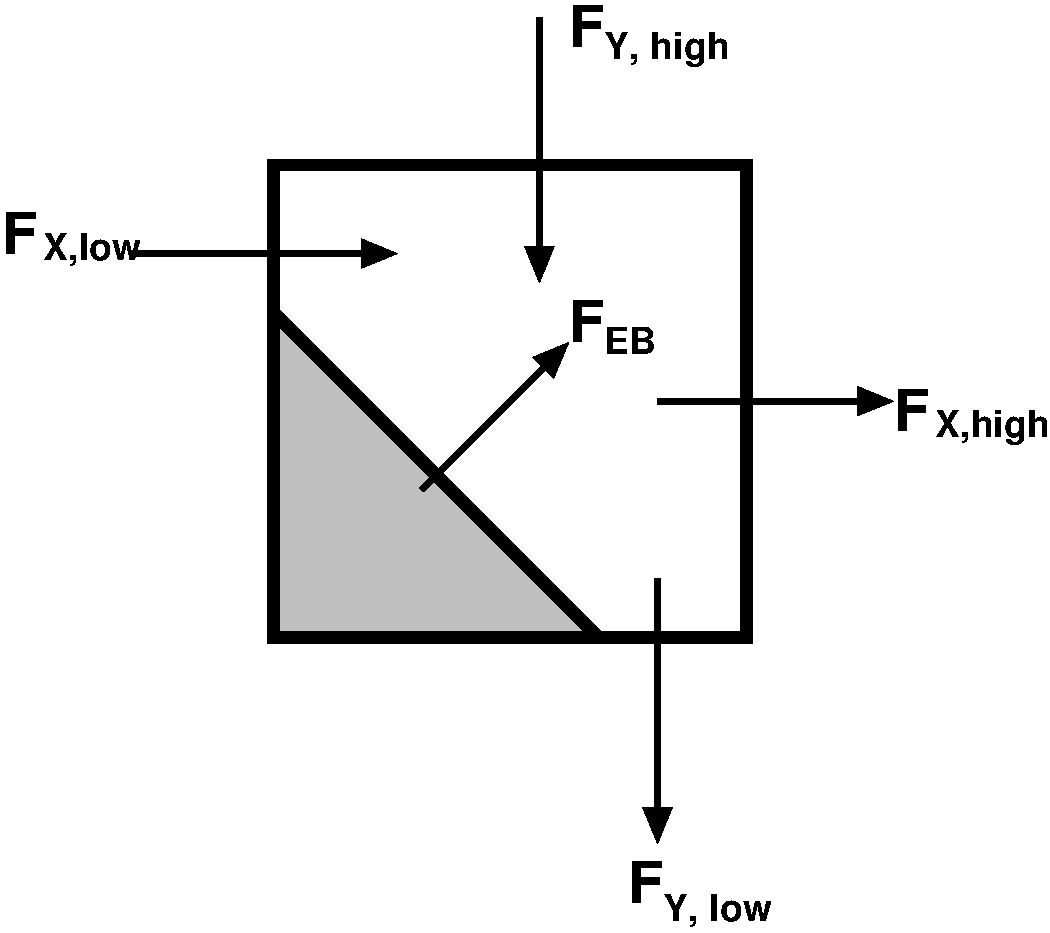
\includegraphics[width=0.25\textwidth]{./EB/eb_fluxes.pdf}
%  \caption{\label{fig::eb_fluxes}The divergence of fluxes in a cut cell.}
%\end{figure}
%\begin{itemize}
%\item
%Volume fractions,
%\item
%Area fractions,
%\item 
%Cell and face centroids
%\end{itemize}

\subsection{Small Cells And Stability}

In the context of time-explicit advance methods for, say hyperbolic conservation laws, 
a naive discretization in time of \ref{eqn::hypsys} using \ref{eqn::ebdiv},
$$
U^{n+1} = U^{n} - \delta t D^c(F)
$$
would have a time step constraint $\dt \sim h \kappa^{1/D}/V_m$,  which
goes to zero as the size of the 
smallest volume fraction $\kappa$ in the calculation.  Since EB volume fractions can
be arbitrarily small, this is an unacceptable constraint.  One way to remedy
this is to create ``non-conservative'' approximation to the divergence
$D^{nc}$, which at a cell $\ibold$, can be formed as an average of the conservative
divergences in the neighborhodd, $N_\ibold$, of $\ibold$.
$$
D^{nc}(F)_\ibold = \frac{\sum_{\jbold \in N_\ibold}\kappa_\jbold D(F)_\jbold}{\sum_{\jbold \in N_\ibold}\kappa_\jbold}
$$
Incorporating this form, the solution can be updated using a {\it hybrid divergence},
$D^H(F) = \kappa D^c(F) + (1-\kappa)D^{nc}$:
$$
U^{n+1,*} = U^n - \delta t D^H(F)
$$
However, we would like our finite-volume scheme to strictly conserve the field quantities
over the domain.  To enforce this, we calculate $\delta M$, the mass gained or
lost by not using $D^c$ directly,
$$
\delta M_\ibold = \kappa (1-\kappa)(D^c(F)_\ibold - D^{nc}(F)_\ibold)
$$
This ``excess material'' (mass, if $U=\rho$) can be {\em redistributed}\ in a time-explicit fashion
to neighboring cells, $\jbold \in N_\ibold$:
$$
\delta M_\ibold = \sum_{\jbold \in N_\ibold} \delta M_{\jbold, \ibold}.
$$
in order to preserve strict conservation over $N_\ibold$.

Note that the physics at hand may impact the optimal choice of precisely how the excess mass is distributed
in this fashion.  We introduce a weighting for redistribution, $W$,
\begin{equation}
\delta M_{\jbold, \ibold} =  \frac{\delta M_\ibold \kappa_\jbold
  W_\jbold}{\sum_{\kbold \in N_\ibold} \kappa_\kbold W_\kbold}
\label{eqn::massweight}
\end{equation}
For all $\jbold \in N_\ibold$,
$$
U^{n+1}_\jbold = U^{n+1,*}_\jbold + 
 \frac{\delta M_\ibold
  W_\jbold}{\sum_{\kbold \in N_\ibold} \kappa_\kbold W_\kbold}.
$$
 Typically, the redistribution neighborhood for each cell is one that can be reached via a monotonic
 path in each coordinate direction of unit length
(see, e.g., Figure~\ref{fig::redistribution})
\begin{figure}[h]
  \centering
  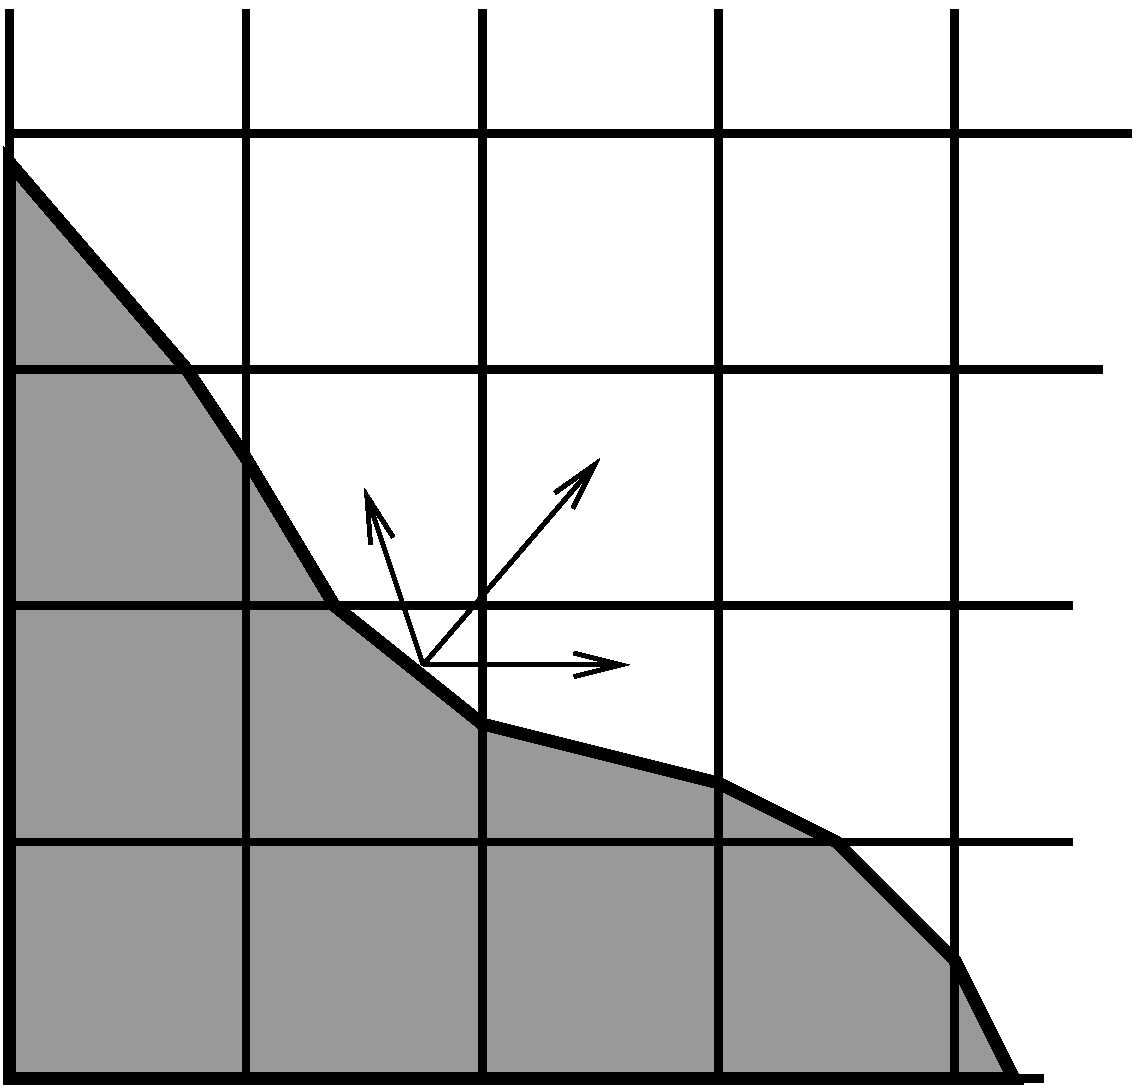
\includegraphics[width=0.25\textwidth]{./EB/redist.pdf}
\caption{\label{fig::redistribution}
Redistribution illustration.  Excess mass due to using a hybrid
divergence $D^H$ instead of the conservative divergence $D^C$ is
distributed to neighbor cells.}
\end{figure}

\section{Initializing \ebis, the Geometric Database}
\label{sec:EB:ebinit}

In $\tt{AMReX}$ the geometric information is stored in a distributed database class, \ebis, which must be
initialized at the start of the calculation.  The procedure for this
goes as follows:
\begin{itemize}
\item Define function of position which describes the surface 
      and use it define a \geom\ object (see \S
      \ref{sec:EB:geometryshop}) -- specifically, the scalar value returned by this function takes on a
      negative value inside the fluid, a positive value in the body, and identically zero at the EB.
\item Construct an \ebis\ with the \geom\ object.   This
  will fill the underlying database of geometric information, specifically tailored to the
  actual meshes that will be used.  Thus, the construction requires one to specify
  the actual mesh resolution that will be used in a calculation.
\end{itemize}

To facilitate the first step, $\tt{AMReX}$ defines a virtual class, an ``implicit function'', \baseif, which encapsulates this functionality.
An instance of a \baseif\ object is required for the construction of a \geom\ object.
\begin{lstlisting}[language=cpp]
    GeometryShop(const BaseIF& a_localGeom)
\end{lstlisting}
Although the user is free to define their own instance of this class, $\tt{AMReX}$ provides a number of preconfigured useful ones.  This
are listed in the next section.

\subsection{Example: Spherical EB}
The spherical implicit function, \sphereif, derives from \baseif, and defines the function
$$
S(\xbold) = x^2 + y^2 + z^2 - R^2,
$$
In this case, the solution domain is defined as the interior of a sphere of radius $R$.
If the sign of $S$ is reversed, the solution domain is the exterior of the sphere.
The following example illustrates how to use the \sphereif\ class to define a \geom\ object:

\begin{lstlisting}[language=cpp]

  int nx = 1024;
  Box domain(IntVect::Zero, (nx-1)*IntVect::Unit);
  Real dx = 1.0/nx;
  Real radius = 0.1;
  Real center = 0.5*RealVect::Unit;
  bool insideRegular = false;
  //this is the implicit function
  SphereIF sphere(radius, center, insideRegular);

  //this is worker object that creates geometric information given an IF
  GeometryShop workshop(sideImpMultisphere)

  //this is the global, distributed database being initialized
  EBIndexSpace*  ebis = AMReX_EBIS::instance()
  ebis->define(domain, RealVect::Zero, dx, workshop);

\end{lstlisting}

In this case, we construct an $r=0.1$ sphere, centered within a unit cube.  The mesh resolution is $1024^3$.
The \geom\ object based on this sphere is then used to construct the \ebis, as shown.

\subsubsection{Other basic shapes:}

\begin{itemize}

\item Planes are made using the class $\tt{PlaneIF}$ which given a normal
$\nbold$  and a center $\cbold$ gives the implicit function 
$$
I(\xbold) = \sum_{1<=d<=D} n_d (x_d - c_d).
$$

\begin{lstlisting}[language=cpp]
RealVect normal; 
RealVect center;
...fill in values for n and c...

PlaneIF plane(normal,point, true);
GeometryShop workshop(plane)

EBIndexSpace*  ebis = AMReX_EBIS::instance()
ebis->define(domain, RealVect::Zero, dx, workshop);

\end{lstlisting}

\item Polynomials of any form can be made using the class
  $\tt{PolynomialIF}$.  Here is an example that makes a parabola of
  the form $I(\xbold) = x - y^2 - z^2$. 
\begin{lstlisting}[language=cpp]

Vector<PolyTerm> poly;
PolyTerm mono;
Real coef;
IntVect powers;
Real amplitude = 1;
// y^2 term
coef = amplitude;
powers = IntVect::Zero;
powers[1] = 2;

mono.coef   = coef;
mono.powers = powers;
poly.push_back(mono);

// z^2 term
coef = amplitude;
            RealVect translation;
      
            for(int idir = 0; idir < SpaceDim; idir++)
            {
              int finesize = finest_domain.size()[idir];
              translation[idir] = 0.5*finesize*fine_dx;
            }
            translation[0] = 0;

            TransformIF implicit(mirror);
            implicit.translate(translation);
            impfunc.reset(implicit.newImplicitFunction());

powers = IntVect::Zero;
powers[2] = 2;
mono.coef   = coef;
mono.powers = powers;
poly.push_back(mono);

// x term
coef = -1.0;
powers = IntVect::Zero;
powers[0] = 1;
mono.coef   = coef;
mono.powers = powers;

poly.push_back(mono);

PolynomialIF mirror(poly,false);
GeometryShop workshop(mirror)
EBIndexSpace*  ebis = AMReX_EBIS::instance()
ebis->define(domain, RealVect::Zero, dx, workshop);
\end{lstlisting}

\end{itemize}
\subsection{Implicit Function Transformation Tools}

More complex domains can be constructed by composing these fundamental shapes.
$\tt{AMReX}$ contains the following classes to compose implicit functions:
\begin{itemize}
\item $\tt{TransformIF}$    allows for translations and rotations of an implicit function.
\item $\tt{UnionIF}$        produces the union of two implicit functions.  
\item $\tt{IntersectionIF}$ produces the intersection of two implicit functions.
\item $\tt{LatheIF}$        creates a 3D implicit function as the surface of
  revolution of a 2D implicit function.
\end{itemize}

\subsection{Multi-sphere example}
The following example creates a geometry using multiple spheres:

\begin{lstlisting}[language=cpp]

vector<Real>     radius(numSpheres);
vector<RealVect> center(numSpheres);
...
//create an implicit function for each sphere
vector<BaseIF*>  spheres(numSpheres);

for(int isphere = 0; isphere < numSpheres; isphere++)
{
  // Create sphere at each origin and translate
  SphereIF sphereAtZero(radius[isphere], RealVect::Zero, false);
  TransformIF* movedSphere = new TransformIF(sphereAtZero);
  movedSphere->translate(center[isphere]);
  spheres[isphere] = static_cast<BaseIF*>(movedSphere);
}
// Create implicit function as intersection of spheres
IntersectionIF impMultisphere(spheres);

// Fluid will in the complement space outside the sphere
ComplementIF sideImpMultisphere(impMultisphere, false);

// Construct the geometryshop
GeometryShop workshop(sideImpMultisphere)
\end{lstlisting}

\subsection{Geometric example 2 -- Surface of revolution}

Here is an example that creates a geometric construction using a
surface of revolution of a set of polygons.   This particular example
only makes sense in three dimensions.   With the right polygons, it
creates the surface shown in \ref{fig::revolution}.

\begin{lstlisting}[language=cpp]

/// define EBIndexSpace from the surface of revolution of a set of polygons
void
defineGeometry(const Real& fine_dx, const  Box& finest_domain, int max_grid_size)
{
  amrex::Print() << "creating geometry from polygon surfaces of revolution" << endl;

  // These  the polygons that get built around the z axis
  Vector<Vector<RealVect> > polygons;
  //....fill the polygons any way you like//

  // Make the Array of (convex) polygons (Arrays of points) into a union
  // of convex polygons, each made from the intersection of a set of half
  // planes/spaces - all represented by implicit functions.

  // A list of all the polygons as implicit functions
  Vector<BaseIF*> polytopes;
  polytopes.resize(0);
  int numPolys = polygons.size();
  // Process each polygon
  for (int p = 0; p < numPolys; p++)
  {
    // All the half planes/spaces used to make a polygon
    Vector<BaseIF*> planes;
    planes.resize(0);

    // Get the current polygon (as a Array of points)
    const Vector<RealVect>& polygon = polygons[p];

    // Get the number of points in the polygon
    int numPts = polygon.size();

    // Process each pair of points
    for (int n = 0; n < numPts; n++)
    {
      // The normal and point is space used to specify each half plane/space
      RealVect normal(RealVect::Zero);
      RealVect point;

      // Set the normal remembering that the last point connects to the first
      // point.
      normal[0] = -(polygon[(n+1) % numPts][1] - polygon[n][1]);
      normal[1] =  (polygon[(n+1) % numPts][0] - polygon[n][0]);

      point = polygon[n];

      // Generate the appropriate half plane/space (as an implicit function)
      PlaneIF* plane;
      plane = new PlaneIF(normal,point,true);

      // Save the result
      planes.push_back(plane);
    }

    // Intersect all the half planes/spaces to create an implicit function
    // that represents the polygon
    IntersectionIF* polygonIF = new IntersectionIF(planes);

    polytopes.push_back(polygonIF);
  }

  //this makes the cross section the union of all the polgons (around
  //z-axis, recall)
  UnionIF crossSection(polytopes);
            
  // In 3D rotate about the z-axis 
  LatheIF lathe(crossSection, false);

  //we are starting around the z axis so we need to translate
  //over to the center of the x-y plane
            
  RealVect translation;
  for(int idir = 0; idir < SpaceDim; idir++)
  {
    translation[idir] = 0.5*finest_domain.size()[idir]*fine_dx;
  }
  translation[2] = 0;
  TransformIF implicit(lathe);
  implicit.translate(translation);

  //create a workshop from translated surface of revolution
  GeometryShop gshop(implicit, false);
  //define th geometric database
  AMReX_EBIS::instance()->define(finest_domain, RealVect::Zero,
                                 fine_dx, gshop, max_grid_size);
}

\end{lstlisting}

\begin{figure}[h]
  \centering
  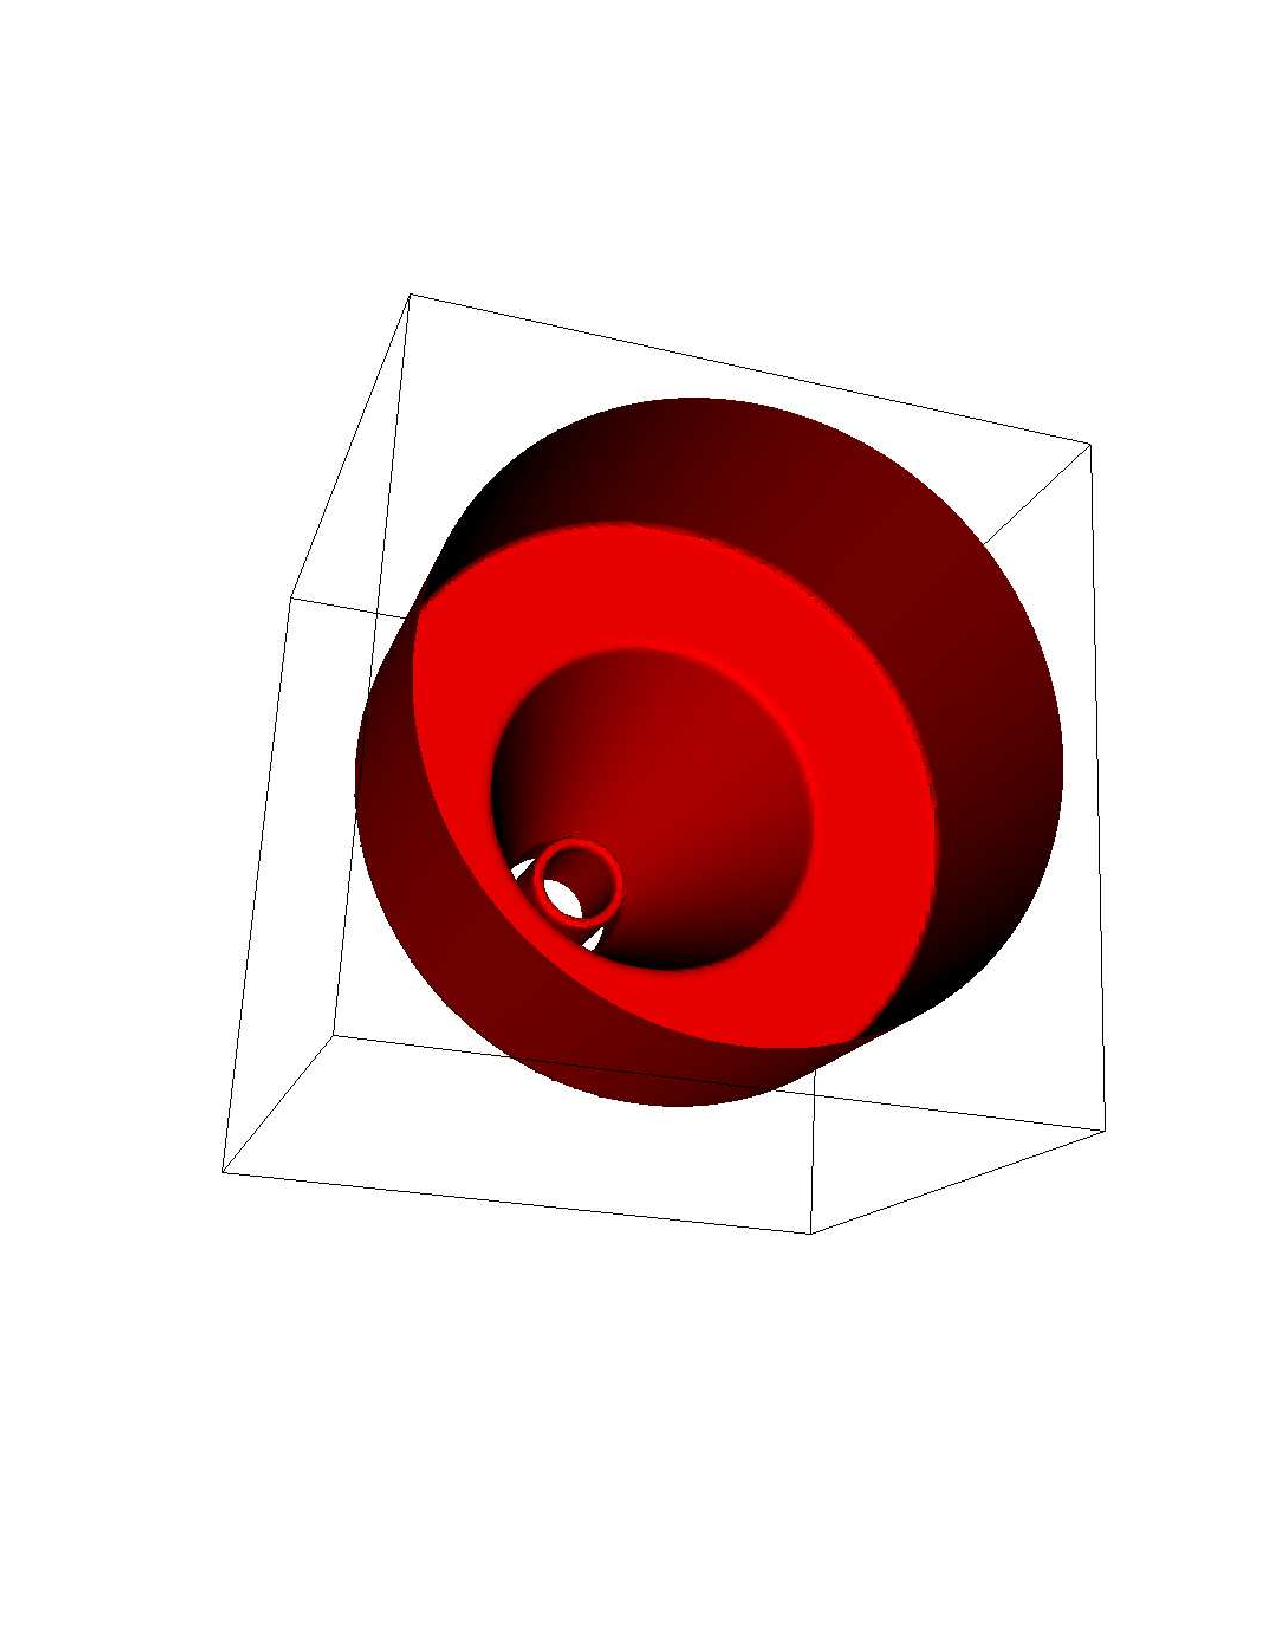
\includegraphics[width=0.375\textwidth]{./EB/revolution.pdf}
  \caption{\label{fig::revolution} Zero surface of an implicit
    function made using a surface of revolution.}
\end{figure}
\subsection{Geometric example 3 -- A Sphere Inside a Parabola}

Here is an example that creates a geometry of a sphere contained
within a parabola. This code
creates the surface shown in \ref{fig::parabolasphere}.

\begin{lstlisting}[language=cpp]
Vector<PolyTerm> poly;

PolyTerm mono;
Real coef;
IntVect powers;
Real amplitude = 1;

// y^2 term
coef = amplitude;
powers = IntVect::Zero;
powers[1] = 2;

mono.coef   = coef;
mono.powers = powers;

poly.push_back(mono);

// z^2 term
coef = amplitude;
powers = IntVect::Zero;
powers[2] = 2;
mono.coef   = coef;
mono.powers = powers;
poly.push_back(mono);

// x term
coef = -1.0;
powers = IntVect::Zero;
powers[0] = 1;
mono.coef   = coef;
mono.powers = powers;

poly.push_back(mono);

PolynomialIF mirror(poly,false);
RealVect translation;

for(int idir = 0; idir < SpaceDim; idir++)
{
  int finesize = finest_domain.size()[idir];
  translation[idir] = 0.5*finesize*fine_dx;
}
RealVect center = translation;
translation[0] = 0;

TransformIF transform(mirror);
transform.translate(translation);

Real radius = 0.2*center[0];
SphereIF sphere(radius, center, true);
Vector<BaseIF*> funcs(2);
funcs[0] = &transform;
funcs[1] = &sphere;
UnionIF implicit(funcs);
impfunc.reset(implicit.newImplicitFunction());
GeometryShop gshop(impfunc, false);
//define th geometric database
AMReX_EBIS::instance()->define(finest_domain, RealVect::Zero,
                                 fine_dx, gshop, max_grid_size);
\end{lstlisting}

\begin{figure}[h]
  \centering
  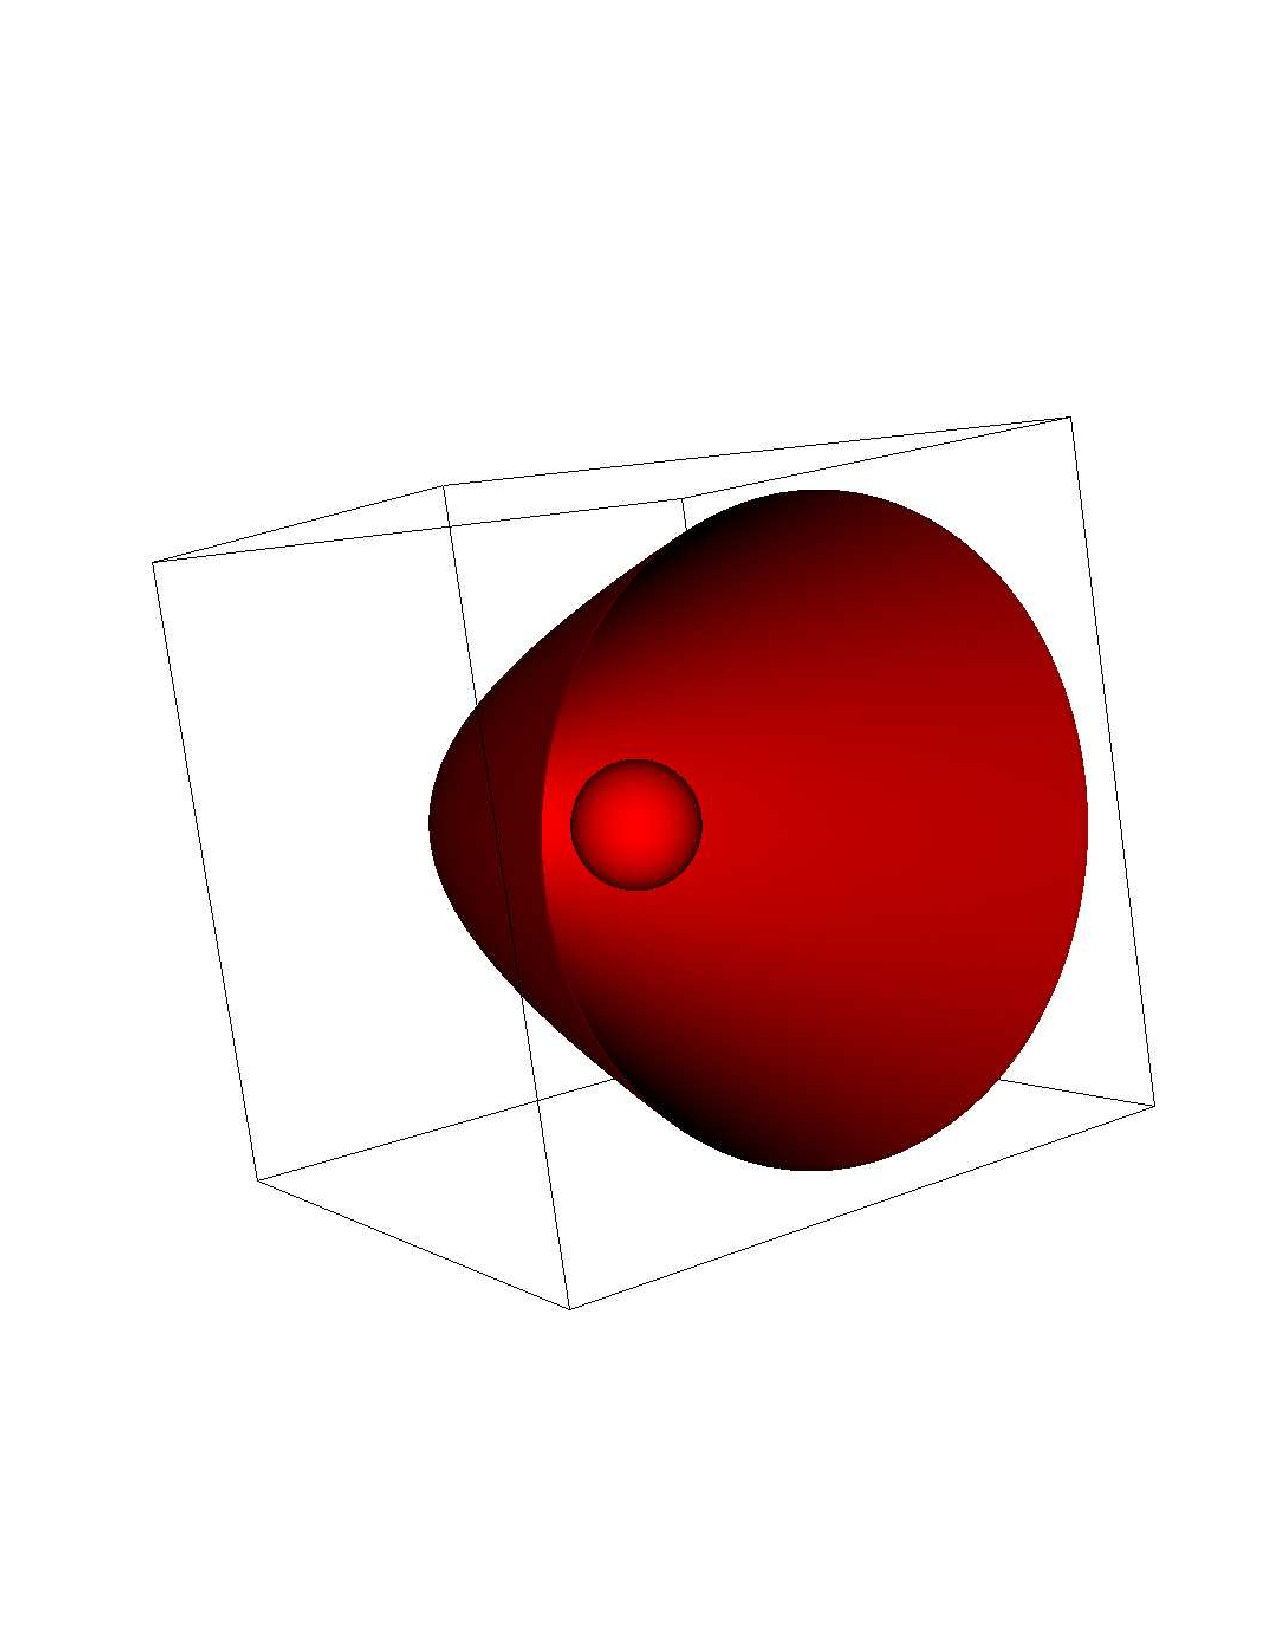
\includegraphics[width=0.375\textwidth]{./EB/parabsphere.pdf}
  \caption{\label{fig::parabolasphere} Zero surface of an implicit
    function made the above code.}
\end{figure}

\section{$\tt{EBFarrayBox}$}

The fundamental data structure for embedded boundary calculations is 
$\tt{EBFArrayBox}$. $\tt{EBFArrayBox}$ is an a $\tt{FArrayBox}$ with two extra
data members.
\begin{itemize}
\item $\tt{EBFArrayBox::getEBISBox}$ returns an $\tt{EBISBox}$, a data
  structure that contains the geometric information of an \ebis\ but
  restricted to a given box.
\item $\tt{EBFArrayBox::getEBCellFlagFab}$  is a
  $\tt{BaseFab<EBCellFlag>}$, where $\tt{EBCellFlag}$ is a class which
  is a class with tools that compactly specifies local cell connectivities
  on a box.
\end{itemize}
If one compiles with $\tt{AMREX\_USE\_EB = TRUE}$, the state data managed by
the ${\tt Amr}$ class is automatically of type $\tt{EBFArrayBox}$ (typically the data
is exposed explicitly as a $\tt{MultiFab}$, but the additional functionality
may be accessed through a C++ type cast. The
$\tt{EBCellFlagFab}$ can be used down in $\tt{Fortran}$, e.g., to choose
locally whether EB-specific operations and data are required for constructing
discretizations.  In the next section, we show examples of this workflow.

\subsection{$\tt{EBFarrayBox}$ Usage Example}
In order to make these EB concepts more concrete, we discuss here sample code
that appears in the $\tt{AMReX}$ tutorial, $\tt{Tutorial/EB/CNS}$.  This code
implements a time-explicit second-order method of lines integrator for hyperbolic
and parabolic transport based on a gamma-law gas EOS and constant transport
properties.  This example also demonstrates how to avoid the more complex/expensive
EB-related logic if the tile under consideration has no cut cells.

\begin{lstlisting}[language=cpp]
void
CNS::compute_dSdt (const MultiFab& S, MultiFab& dSdt, Real dt,
                   EBFluxRegister* fr_as_crse, EBFluxRegister* fr_as_fine)
{
    BL_PROFILE("CNS::compute_dSdt()");

    const Real* dx = geom.CellSize();
    const int ncomp = dSdt.nComp();

#ifdef _OPENMP
#pragma omp parallel
#endif
     {
        //fluxes for the advance
        std::array<FArrayBox,AMREX_SPACEDIM> flux;

        for (MFIter mfi(S, MFItInfo().EnableTiling(hydro_tile_size).SetDynamic(true));
                        mfi.isValid(); ++mfi)
        {
            //this tile is the subset of the box over which we are computing
            const Box& bx = mfi.tilebox();

            //because we have compiled with AMREX_USE=EB_TRUE, the
            //MultiFab holds EBFArrayBox(es) so we can do this cast
            const EBFArrayBox& sfab
                = dynamic_cast<EBFArrayBox const&>(S[mfi]);
            
            //here we are getting the collection of flags so we know
            //kind of grid this is and if it is an EB grid, we have
            //the connectivity info
            const EBCellFlafgFab & flag = sfab.getEBCellFlagFab();

            if (flag.getType(bx) == FabType::covered) 
            {
              //this tile is covered so there are no meaningful data here
                dSdt[mfi].setVal(0.0, bx, 0, ncomp);
            } 
            else 
            {
              //create the flux holders for this tile
              for (int idim=0; idim < AMREX_SPACEDIM; ++idim) 
              {
                flux[idim].resize(amrex::surroundingNodes(bx,idim),ncomp);
              }

              if (flag.getType(amrex::grow(bx,1)) == FabType::regular)
              {
                //this tile has no cut cells so we can just proceed
                //with a (cheaper) non-eb call

                cns_compute_dudt(BL_TO_FORTRAN_BOX(bx),
                BL_TO_FORTRAN_ANYD(dSdt[mfi]),
                BL_TO_FORTRAN_ANYD(S[mfi]),
                BL_TO_FORTRAN_ANYD(flux[0]),
                BL_TO_FORTRAN_ANYD(flux[1]),
                BL_TO_FORTRAN_ANYD(flux[2]),
                dx, &dt);

              }
              else
              {
                //this tile has cut cells so we have to send into Fortran
                //EBCellFlagFAB as well as lots of geometric
                //information
                //the areafrac and facecent objects are member data
                //filled using EBISBox
                cns_eb_compute_dudt(BL_TO_FORTRAN_BOX(bx),
                BL_TO_FORTRAN_ANYD(dSdt[mfi]),
                BL_TO_FORTRAN_ANYD(S[mfi]),
                BL_TO_FORTRAN_ANYD(flux[0]),
                BL_TO_FORTRAN_ANYD(flux[1]),
                BL_TO_FORTRAN_ANYD(flux[2]),
                BL_TO_FORTRAN_ANYD(flag),
                BL_TO_FORTRAN_ANYD(volfrac[mfi]),
                BL_TO_FORTRAN_ANYD(bndrycent[mfi]),
                BL_TO_FORTRAN_ANYD(areafrac[0][mfi]),
                BL_TO_FORTRAN_ANYD(areafrac[1][mfi]),
                BL_TO_FORTRAN_ANYD(areafrac[2][mfi]),
                BL_TO_FORTRAN_ANYD(facecent[0][mfi]),
                BL_TO_FORTRAN_ANYD(facecent[1][mfi]),
                BL_TO_FORTRAN_ANYD(facecent[2][mfi]),
                dx, &dt);
              }
            }
          }
        }

\end{lstlisting}

This is the main loop in the routine to advance the state.  The state, $\tt{S}$, comes into this routine with grow cells
properly filled, and this routine features a $\tt{MultiFab}$ iterator loop to step through this data, tile-by-tile and compute
$\tt{dSdt}$.  Here, we see that the definition of $\tt{sfab}$ incorporates the aforementioned type cast, enabling queries about
the EB nature of the data.  Of the two possiblities handled, the ``regular'' type without cut cells has a much simpler interface.
The EB version takes all the same data, but additionally requires (dense) data to specify the volume and face area fractions,
centroid information, and the $\tt{flag}$ structure that will be queried pointwise for the local cell connectivity.

\subsection{Fortran code Snippets}
Much of the code to compute these fluxes and their divergence in this example is too detailed to step through in this context.
There are however a few salient features worth pointing out.

\subsubsection{The data is cell-centered, even cut cells}
In order to simplify the construction second-order discretizations, we can base all the numerical operations on the assumption
that all cell-based data lives at the center of the {\em full}\ cell containing the cut cells.  This means that when we take a
standard centered difference between cell data at $(i,j,k)$ and $(i+1,j,k)$, e.g., we get a gradient value that is second-order and
centered on the full face at $i+1/2$, regardless of the aperature.

\subsubsection{Many EB operations can be organized as post-processing}
Recall that a second-order finite-volume scheme requires that fluxes
be centered on the face {\em centroid}.  This can be accomplished by post-processing face-centered fluxes with a linear interpolation
of adjacent face values.  The resulting centroid-based fluxes are second-order, and can be used to construct the conservative
divergence we seek.  Note that this operation requires the location of the face centroids, and increases the grow cell requirement
of the flux operators, as does the necessity to form the {\em hybrid divergence}\ operator discussed above.

\subsubsection{The $\tt{flag}$ data}
$\tt{AMReX}$ provides functions that query the $\tt{flag}$ data in order to infer the local connectivity of cells.  For example,
the cell itself or its neighbors may be covered or cut.  If cut, the data is centered at the center of the full cell.  If covered,
the data is invalid and should not be involved in the fluid advance.  An example of such a call is:

\begin{lstlisting}[language=Fortran]
   call get_neighbor_cells(cellflag(i,j,k),nbr)
\end{lstlisting}

Here, for the $\tt{flag}$ at $(i,j,k)$ is used to fill a local $3^3$ array of integers with the value $1$ if connected to $(i,j,k)$,
and $0$ if not.  Similar queries:

\begin{lstlisting}[language=Fortran]
   is_covered_cell(cellflag(i,j,k))
   is_single_valued_cell(cellflag(i,j,k)
\end{lstlisting}
can be used to gather additional detail.

Below, we show a partial listing of the $\tt{cns_eb_compute_dudt}$ code, specifically after the face-centered fluxes have been computed,
and showing part of the work necessary to interpolate them to face centroids (while appropriately handling covered data).

\begin{lstlisting}[language=Fortran]
    do n = 1, ncomp

       !
       ! First, we compute conservative divergence on (lo-2,hi+2)
       !
       iwall = 0
       do       k = lo(3)-2, hi(3)+2
          do    j = lo(2)-2, hi(2)+2
             do i = lo(1)-2, hi(1)+2
                divc(i,j,k) = (fluxx(i,j,k,n)-fluxx(i+1,j,k,n))*dxinv(1) &
                     +        (fluxy(i,j,k,n)-fluxy(i,j+1,k,n))*dxinv(2) &
                     +        (fluxz(i,j,k,n)-fluxz(i,j,k+1,n))*dxinv(3)
             end do

             do i = lo(1)-2, hi(1)+2
                if (is_covered_cell(cellflag(i,j,k))) then
                   divc(i,j,k) = 0.d0
                else if (is_single_valued_cell(cellflag(i,j,k))) then

                   call get_neighbor_cells(cellflag(i,j,k),nbr)

                   ! x-direction lo face
                   if (apx(i,j,k).lt.1.d0) then
                      if (centx_y(i,j,k).le.0.d0) then
                         fracy = -centx_y(i,j,k)*nbr(0,-1,0)
                         if(centx_z(i,j,k).le. 0.0d0)then
                            fracz = - centx_z(i,j,k)*nbr(0,0,-1)
                            fxm = (1.d0-fracz)*(     fracy *fluxx(i,j-1,k  ,n)  + &
                                 &             (1.d0-fracy)*fluxx(i,j  ,k  ,n)) + &
                                 &      fracz *(     fracy *fluxx(i,j-1,k-1,n)  + &
                                 &             (1.d0-fracy)*fluxx(i,j  ,k-1,n))
                         else
                            fracz =  centx_z(i,j,k)*nbr(0,0,1)
                            fxm = (1.d0-fracz)*(     fracy *fluxx(i,j-1,k  ,n)  + &
                                 &             (1.d0-fracy)*fluxx(i,j  ,k  ,n)) + &
                                 &      fracz *(     fracy *fluxx(i,j-1,k+1,n)  + &
                                 &             (1.d0-fracy)*fluxx(i,j  ,k+1,n))
                         endif
                      else
                         fracy = centx_y(i,j,k)*nbr(0,1,0)
                         if(centx_z(i,j,k).le. 0.0d0)then
                            fracz = -centx_z(i,j,k)*nbr(0,0,-1)
                            fxm = (1.d0-fracz)*(     fracy *fluxx(i,j+1,k  ,n)  + &
                                 &             (1.d0-fracy)*fluxx(i,j  ,k  ,n)) + &
                                 &      fracz *(     fracy *fluxx(i,j+1,k-1,n)  + &
                                 &             (1.d0-fracy)*fluxx(i,j  ,k-1,n))
                         else
                            fracz = centx_z(i,j,k)*nbr(0,0,1)
                            fxm = (1.d0-fracz)*(     fracy *fluxx(i,j+1,k  ,n)  + &
                                 &             (1.d0-fracy)*fluxx(i,j  ,k  ,n)) + &
                                 &      fracz *(     fracy *fluxx(i,j+1,k+1,n)  + &
                                 &             (1.d0-fracy)*fluxx(i,j  ,k+1,n))
                         endif
                      end if
                   else
                      fxm = fluxx(i,j,k,n)
                   end if

           <..... similar code for other fluxes removed ....>

                   iwall = iwall + 1
                   if (n .eq. 1) then
                      call compute_hyp_wallflux(divhyp(:,iwall), i,j,k, q(i,j,k,qrho), &
                           q(i,j,k,qu), q(i,j,k,qv), q(i,j,k,qw), q(i,j,k,qp), &
                           apx(i,j,k), apx(i+1,j,k), &
                           apy(i,j,k), apy(i,j+1,k), &
                           apz(i,j,k), apz(i,j,k+1))
                      call compute_diff_wallflux(divdiff(:,iwall), dxinv, i,j,k, &
                           q, qlo, qhi, &
                           lam, mu, xi, clo, chi, &
                           bcent, blo, bhi, &
                           apx, axlo, axhi, &
                           apy, aylo, ayhi, &
                           apz, azlo, azhi)
                   end if

                   divwn = divhyp(n,iwall) + divdiff(n,iwall)

                   ! we assume dx == dy == dz
                   divc(i,j,k) = -((apx(i+1,j,k)*fxp - apx(i,j,k)*fxm) * dxinv(1) &
                        +          (apy(i,j+1,k)*fyp - apy(i,j,k)*fym) * dxinv(2) &
                        +          (apz(i,j,k+1)*fzp - apz(i,j,k)*fzm) * dxinv(3) &
                        +          divwn * dxinv(1)) / vfrac(i,j,k)
                end if
             end do
          end do
       end do

\end{lstlisting}

One can easily identify the logic and portions of the code devoted toward the EB corrections.  Note, in particular,
that diffusive fluxes into the EB need only be computed on cut cells.

\subsubsection{There are many approaches}
The ``fixes'' that need to occur in these EB algorithms can be managed in a number of ways, depending on the
needs of the application and programming style.  In this example, the geometrical data is used to fill dense
data structures so that the sparse geometry information is available uniformally over the entire box.
Also, the cell types are queried point-by-point in order to form the appropriate stencil. Obviously then
there is a performance penalty if many of the cells in tile are not actually cut.  There is clearly a trade-off
in such designs.  Alternatively, one might build sparse data structures similar to those $\tt{AMReX}$ uses to manage
particles, and apply the EB corrections on this sparse set directly.  Future releases of $\tt{AMReX}$ will
feature an expanded set of EB tutorials to demonstrate an evolving set of tools provided.


\chapter{Visualization}\label{Chap:Visualization}
There are several visualization tools that can be used for \amrex\
plotfiles.  The popular \visit\ package supports the \amrex\ file 
format natively (using the {\sf BoxLib2d} and {\sf BoxLib3d} file types),
as does the \yt\ python package.  The standard tool used within the
\amrex-community is \amrvis, a package developed and supported 
by CCSE that is designed specifically for highly efficient visualization
of block-structured hierarchical AMR data.

\section{\amrvis}

Our favorite visualization tool is \amrvis. We heartily encourage you
to build the {\tt amrvis2d} and {\tt amrvis3d} executables, and to try using them
to visualize your data. A very useful feature is View/Dataset, which
allows you to actually view the numbers in a spreadsheet that is nested
to reflect the AMR hierarchy -- this can be handy for
debugging. You can modify how many levels of data you want to see,
whether you want to see the grid boxes or not, what palette you use,
etc.  Here are some instructions and tips for using \amrvis:

\begin{enumerate}

\item Download and build \amrvis:
\begin{verbatim}
git clone https://ccse.lbl.gov/pub/Downloads/Amrvis.git
\end{verbatim}

Then {\tt cd} into {\tt Amrvis/}, edit the {\tt GNUmakefile} by
setting {\tt COMP} to the compiler suite you have.

Type {\tt make DIM=2} or {\tt make DIM=3} to build, 
resulting in an executable that looks like {\tt amrvis2d...ex}.

If you want to build amrvis with {\tt DIM=3}, you must first
download and build {\tt volpack}:
\begin{verbatim}
git clone https://ccse.lbl.gov/pub/Downloads/volpack.git
\end{verbatim}

Then {\tt cd} into {\tt volpack/} and type {\tt make}.

Note: \amrvis\ requires the OSF/Motif libraries and headers. If you don't have these 
you will need to install the development version of motif through your package manager. 
{\tt lesstif} gives some functionality and will allow you to build the amrvis executable, 
but \amrvis\ may exhibit subtle anomalies.

On most Linux distributions, the motif library is provided by the
{\tt openmotif} package, and its header files (like {\tt Xm.h}) are provided
by {\tt openmotif-devel}. If those packages are not installed, then use the
OS-specific package management tool to install them. 

You may then want to create an alias to {\tt amrvis2d}, for example
\begin{verbatim}
alias amrvis2d /tmp/Amrvis/amrvis2d...ex
\end{verbatim}

\item Run the command {\tt cp Amrvis/amrvis.defaults \textasciitilde/.amrvis.defaults}.
Then, in your copy, edit the line containing ``{\tt palette}'' line to point to, e.g., 
``{\tt palette  /home/username/Amrvis/Palette}''.  The other lines control
options such as the initial field to display, the number format, widow size, etc.
If there are multiple instances of the same option, the last option takes precedence.

\item Generally the plotfiles have the form {\tt pltXXXXX} 
  (the {\tt plt} prefix can be changed), where {\tt XXXXX} is a number 
  corresponding to the timestep the file
  was output.  {\tt amrvis2d <filename>} or {\tt amrvis3d <filename>}
  to see a single plotfile, 
  or for 2D data sets, {\tt amrvis2d -a plt*}, which will animate the 
  sequence of plotfiles.

  You can use the ``Variable'' menu to change the variable.
  You can left-click drag a box around a region
  and click "View'' $\rightarrow$ ``Dataset''
  in order to look at the actual numerical values
  (see Figure \ref{Fig:Amrvis}).
  Or you can simply left click on a point to obtain the numerical value.
  You can also export the
  pictures in several different formats under "File/Export".
  In 2D you can right and center click to get line-out plots.
  In 3D you can right and center click to change the planes, and the hold
  shift+(right or center) click to get line-out plots.

\begin{figure}[tb]
\centering
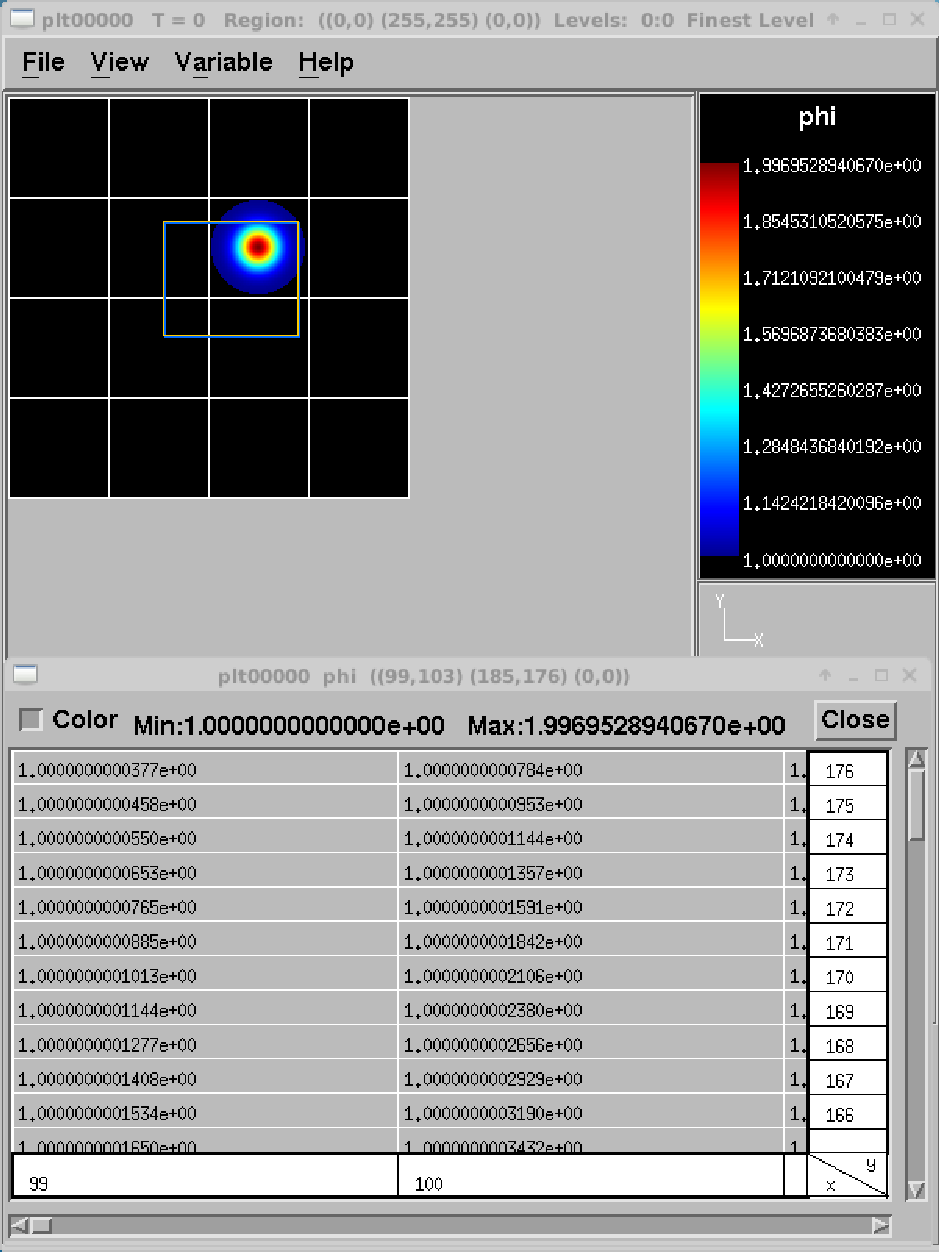
\includegraphics[width=2.5in]{./Visualization/Amrvis_2d}
~~~
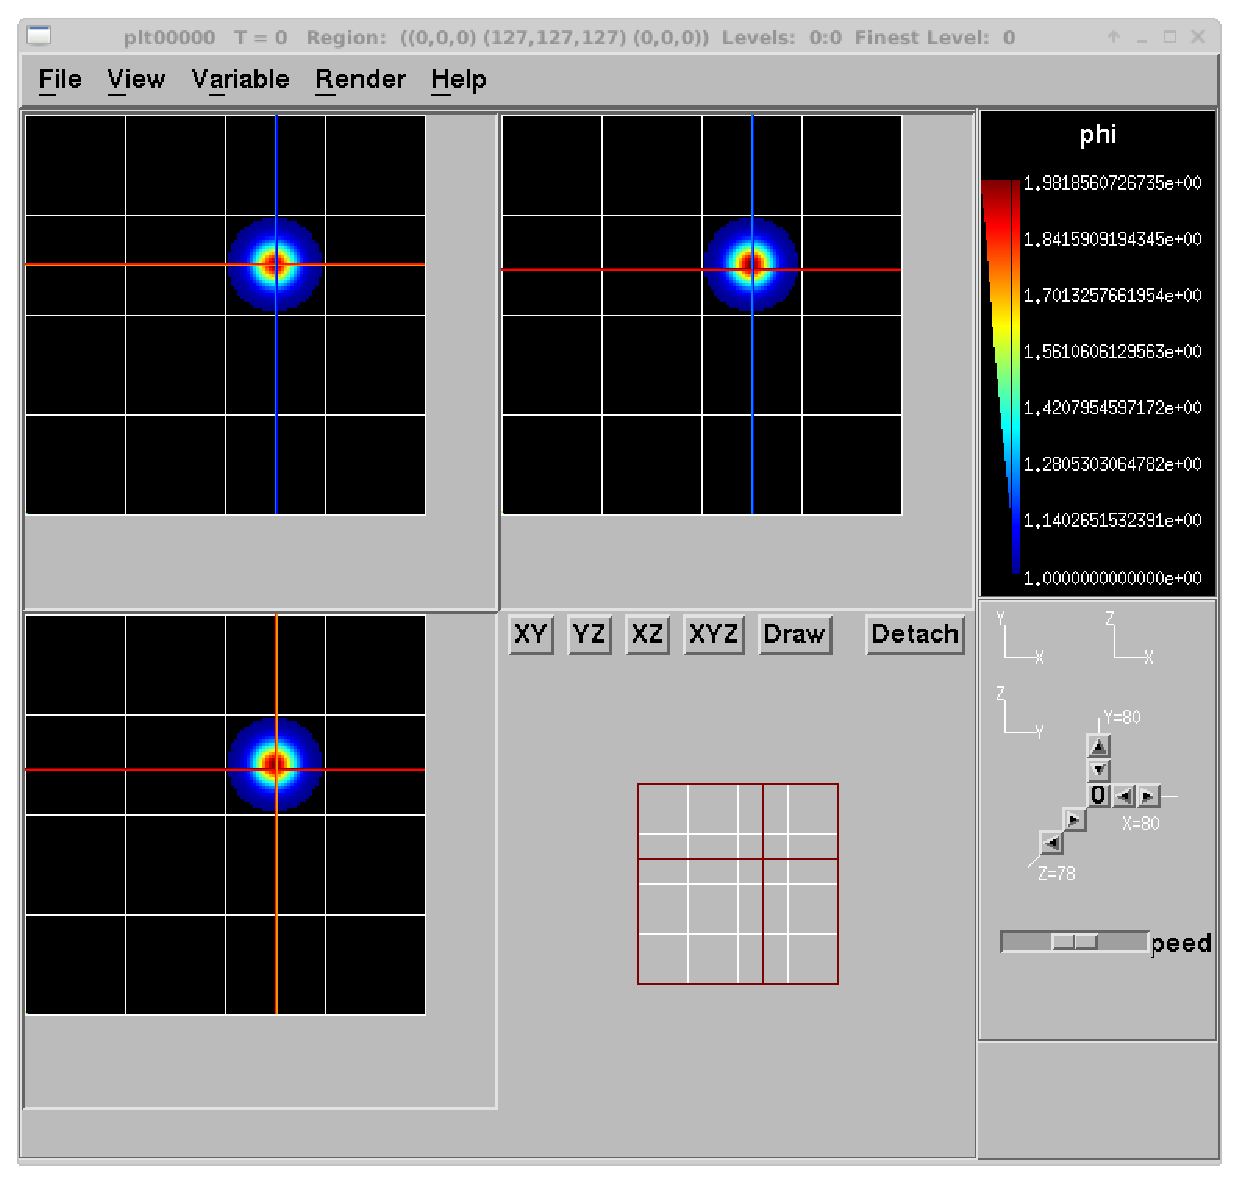
\includegraphics[width=2.5in]{./Visualization/Amrvis_3d}
\caption{2D and 3D images generated with Amrvis}
\label{Fig:Amrvis}
\end{figure}

  We have created a number of routines to convert \amrex\ plotfile data
  other formats (such as MATLAB), but in order to properly interpret 
  the hierarchical AMR data, each tends to have its own idiosyncrasies.
  If you would like to display the data in another format, please contact
  Marc Day ({\tt MSDay@lbl.gov}) and we will point you to whatever we have
  that can help.

\end{enumerate}

\section{\visit}
\label{sec:visit}

\amrex\ data can also be visualized by {\tt VisIt}, an open
source visualization and analysis software.  To follow along with this example,
first build and run the first heat equation tutorial code
(see Section \ref{sec:heat equation}).

Next, download and install {\tt VisIt} from \url{https://wci.llnl.gov/simulation/computer-codes/visit}.
To open a single plotfile, run {\tt VisIt}, then select ``File'' $\rightarrow$ ``Open file ...'',
then select the {\tt Header} file associated the the plotfile of interest (e.g., {\tt plt00000/Header}).
Assuming you ran the simulation in 2D, here are instructions for making a simple plot:
\begin{itemize}
\item To view the data, select ``Add'' $\rightarrow$ ``Pseudocolor'' $\rightarrow$ ``phi'', and then select
``Draw''.
\item To view the grid structure (not particularly interesting yet, but when we add AMR it will be), select
`` $\rightarrow$ ``subset'' $\rightarrow$ ``levels''.  Then double-click the text ``Subset - levels'',
enable the ``Wireframe'' option, select ``Apply'', select ``Dismiss'', and then select ``Draw''.
\item To save the image, select ``File'' $\rightarrow$ ``Set save options'', then customize the image format
to your liking, then click ``Save''.
\end{itemize}
Your image should look similar to the left side of Figure \ref{Fig:VisIt}.\\
\begin{figure}[tb]
\centering
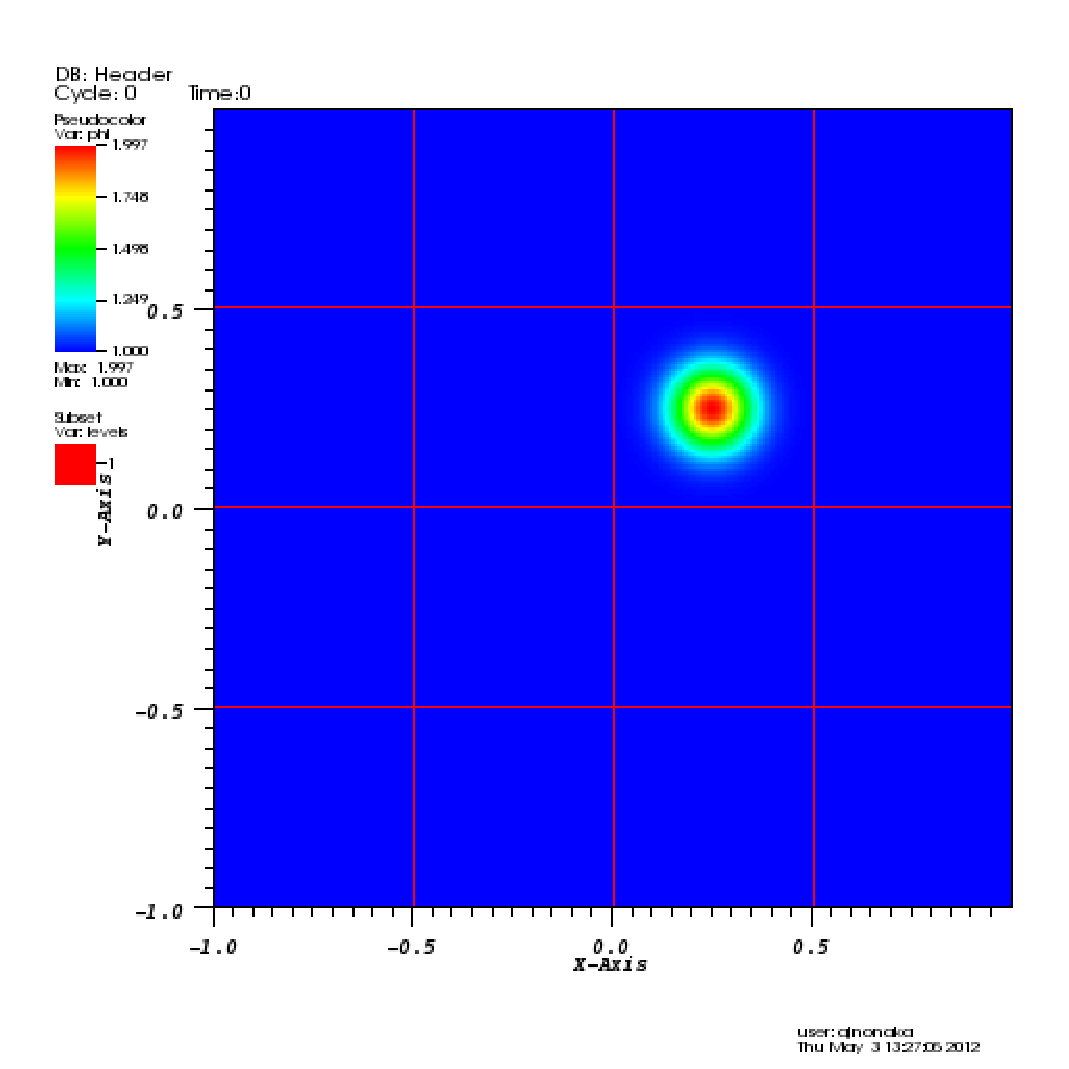
\includegraphics[width=3.1in]{./Visualization/VisIt_2D}
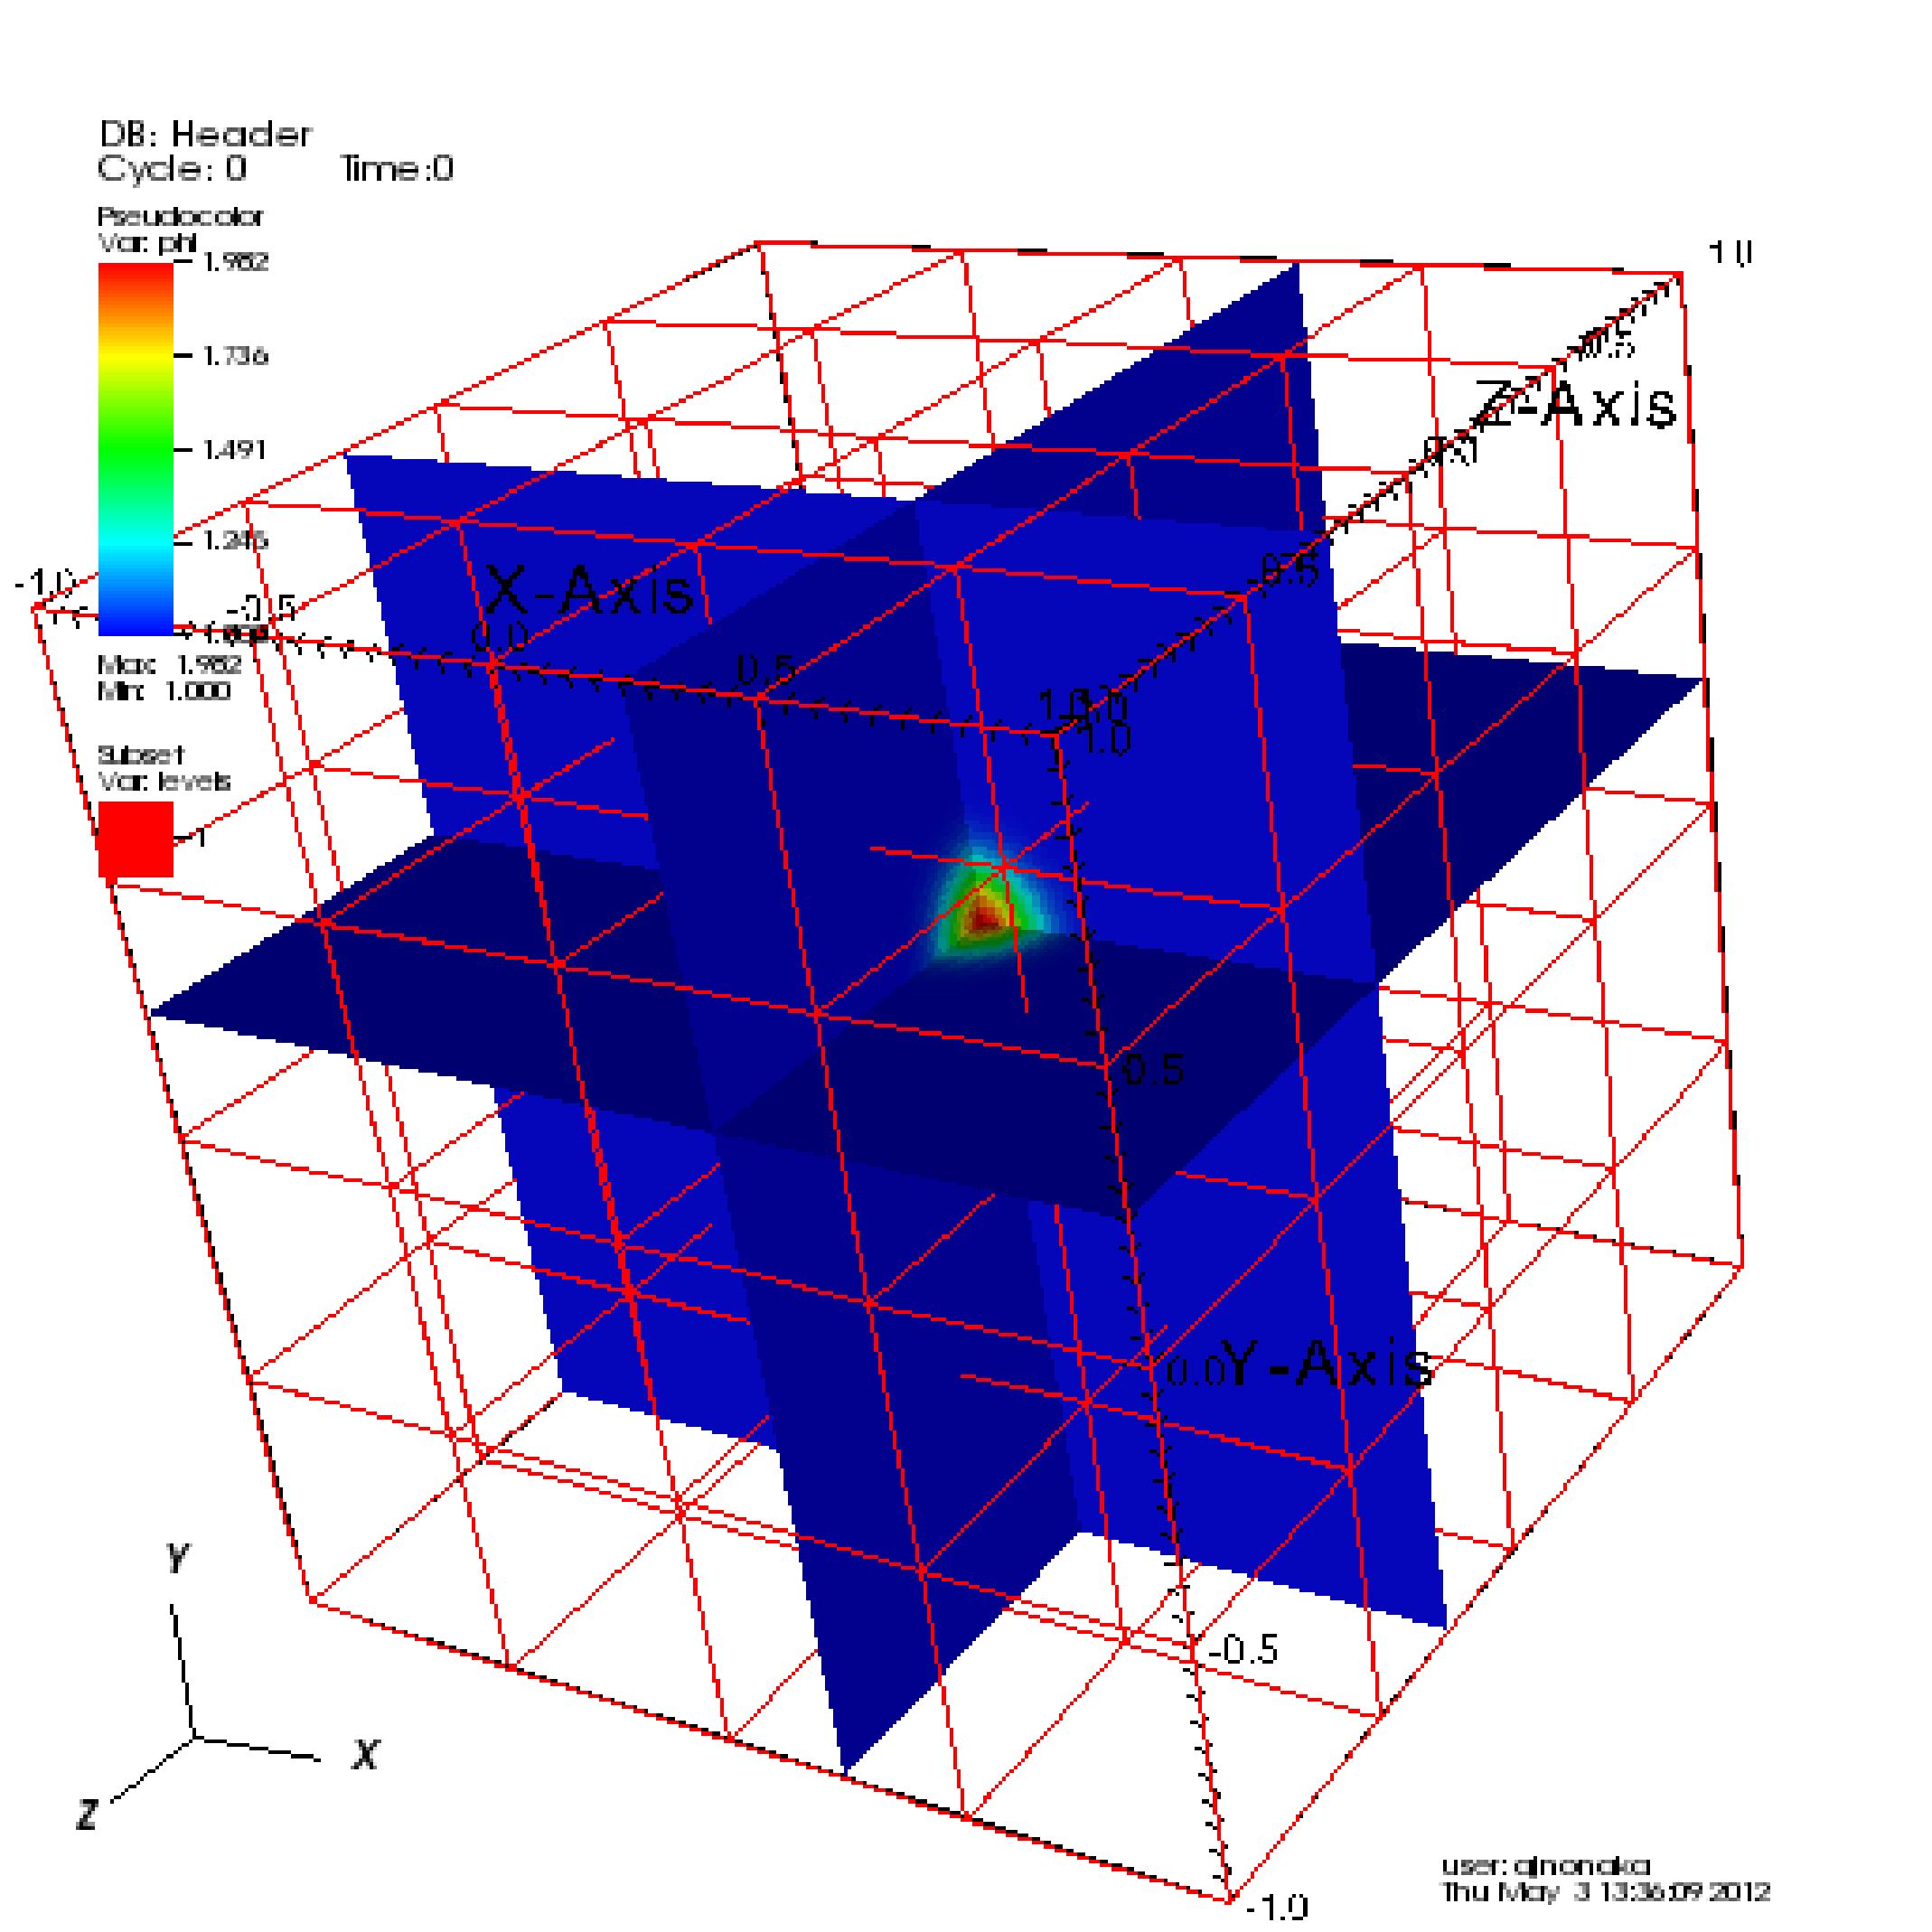
\includegraphics[width=3.1in]{./Visualization/VisIt_3D}
\caption{(Left) 2D image generated with VisIt.  (Right) 3D image generated with VisIt.}
\label{Fig:VisIt}
\end{figure}

In 3D, you must apply the ``Operators'' $\rightarrow$ ``Slicing'' $\rightarrow$ ``ThreeSlice'', with the 
``ThreeSlice operator attribute'' set to x=0.25, y=0.25, and z=0.25.  You can left-click and drag
over the image to rotate the image to generate something similar to right side of Figure \ref{Fig:VisIt}.\\

To make a movie, you must first create a text file named {\tt movie.visit} with a list of the {\tt Header} 
files for the individual frames.  This can most easily be done using the command:
\begin{lstlisting}[backgroundcolor=\color{light-red}]
~/amrex/Tutorials/Basic/HeatEquation_EX1_C> ls -1 plt*/Header | tee movie.visit
plt00000/Header
plt01000/Header
plt02000/Header
plt03000/Header
plt04000/Header
plt05000/Header
plt06000/Header
plt07000/Header
plt08000/Header
plt09000/Header
plt10000/Header
\end{lstlisting}
The next step is to run {\tt VisIt}, select ``File'' $\rightarrow$ ``Open file ...'',
then select {\tt movie.visit}.  Create an image to your liking and press the ``play'' button
on the VCR-like control panel to preview all the frames.  To save the movie, choose
``File'' $\rightarrow$ ``Save movie ...'', and follow the on-screen instructions.

\section{\yt}

\yt, an open source Python package available at \url{http://yt-project.org/},
can be used for analyzing and visualizing mesh and particle data generated by
\amrex\ codes.  Some of the \amrex\ developers are also \yt\ project members.
Below we describe how to use \yt\ on both a local workstation, as well as at
the NERSC HPC facility for high-throughput visualization of large data sets.

\subsection{Using \yt\ on a local workstation}

Running \yt\ on a local system generally provides good interactivity, but
limited performance. Consequently, this configuration is best when doing
exploratory visualization (e.g., experimenting with camera angles, lighting,
and color schemes) of small data sets.

To use \yt\ on an \amrex\ plot file, first start a Jupyter notebook or an IPython kernel, and import the \texttt{yt} module:

\begin{lstlisting}[language=python,breaklines=true]
In [1]: import yt

In [2]: print(yt.__version__)
3.4-dev
\end{lstlisting}

Next, load a plot file; in this example we use a plot file from the Nyx cosmology application:

\begin{lstlisting}[language=python,breaklines=true]
In [3]: ds = yt.load("plt00401")
yt : [INFO     ] 2017-05-23 10:03:56,182 Parameters: current_time              = 0.00605694344696544
yt : [INFO     ] 2017-05-23 10:03:56,182 Parameters: domain_dimensions         = [128 128 128]
yt : [INFO     ] 2017-05-23 10:03:56,182 Parameters: domain_left_edge          = [ 0.  0.  0.]
yt : [INFO     ] 2017-05-23 10:03:56,183 Parameters: domain_right_edge         = [ 14.24501  14.24501  14.24501]

In [4]: ds.field_list
Out[4]:
[('DM', 'particle_mass'),
 ('DM', 'particle_position_x'),
 ('DM', 'particle_position_y'),
 ('DM', 'particle_position_z'),
 ('DM', 'particle_velocity_x'),
 ('DM', 'particle_velocity_y'),
 ('DM', 'particle_velocity_z'),
 ('all', 'particle_mass'),
 ('all', 'particle_position_x'),
 ('all', 'particle_position_y'),
 ('all', 'particle_position_z'),
 ('all', 'particle_velocity_x'),
 ('all', 'particle_velocity_y'),
 ('all', 'particle_velocity_z'),
 ('boxlib', 'density'),
 ('boxlib', 'particle_mass_density')]
\end{lstlisting}

From here one can make slice plots, 3-D volume renderings, etc. An example of
the slice plot feature is shown below:

\begin{lstlisting}[language=python,breaklines=true]
In [9]: slc = yt.SlicePlot(ds, "z", "density")
yt : [INFO     ] 2017-05-23 10:08:25,358 xlim = 0.000000 14.245010
yt : [INFO     ] 2017-05-23 10:08:25,358 ylim = 0.000000 14.245010
yt : [INFO     ] 2017-05-23 10:08:25,359 xlim = 0.000000 14.245010
yt : [INFO     ] 2017-05-23 10:08:25,359 ylim = 0.000000 14.245010

In [10]: slc.show()

In [11]: slc.save()
yt : [INFO     ] 2017-05-23 10:08:34,021 Saving plot plt00401_Slice_z_density.png
Out[11]: ['plt00401_Slice_z_density.png']
\end{lstlisting}

The resulting image is Figure~\ref{fig:yt_Nyx_slice_plot}. One can also make
volume renderings with \yt; an example is show below:

\begin{figure}
  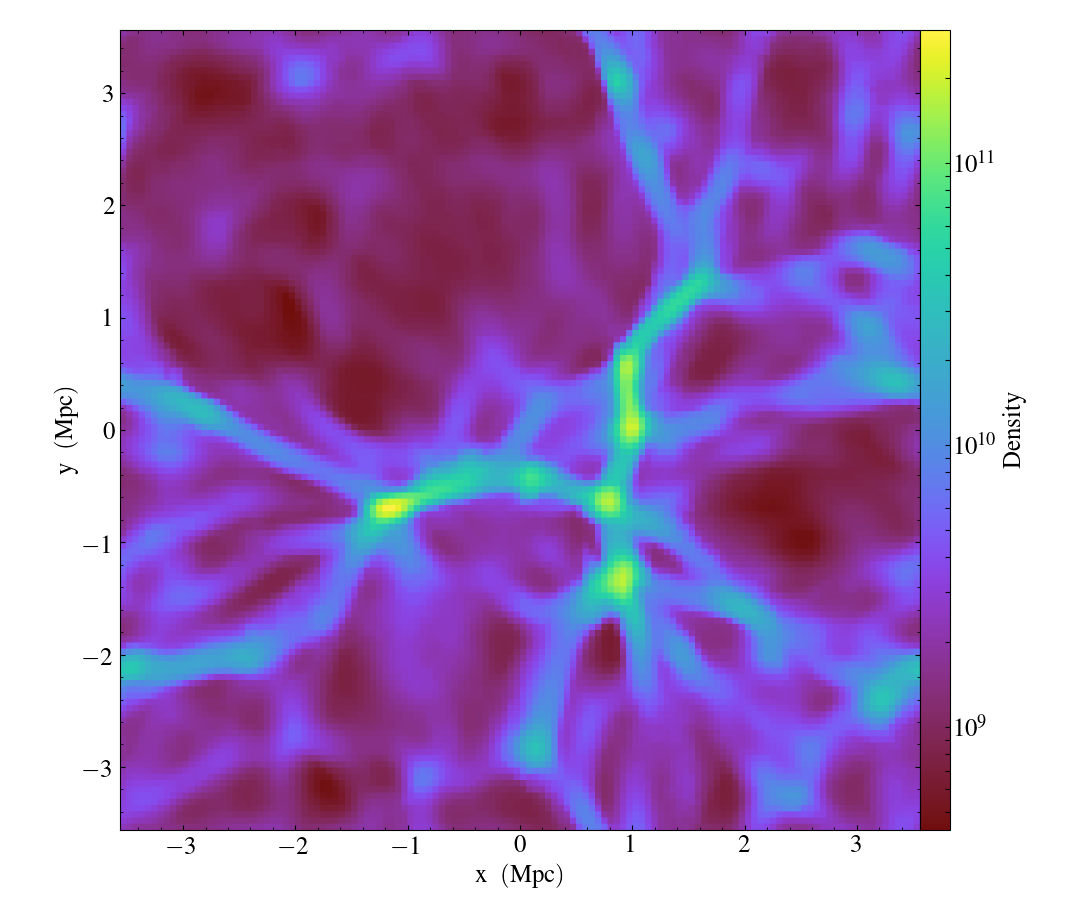
\includegraphics[scale=0.5]{./Visualization/yt_Nyx_density_slice.png}
  \caption{Slice plot of $128^3$ Nyx simulation using \yt.}
  \label{fig:yt_Nyx_slice_plot}
\end{figure}

\begin{lstlisting}[language=python,breaklines=true]
In [12]: sc = yt.create_scene(ds, field="density", lens_type="perspective")

In [13]: source = sc[0]

In [14]: source.tfh.set_bounds((1e8, 1e15))

In [15]: source.tfh.set_log(True)

In [16]: source.tfh.grey_opacity = True

In [17]: sc.show()
<Scene Object>:
Sources:
    source_00: <Volume Source>:YTRegion (plt00401): , center=[  1.09888770e+25   1.09888770e+25   1.09888770e+25] cm, left_edge=[ 0.  0.  0.] cm, right_edge=[  2.19777540e+25   2.19777540e+25   2.19777540e+25] cm transfer_function:None
Camera:
    <Camera Object>:
	position:[ 14.24501  14.24501  14.24501] code_length
	focus:[ 7.122505  7.122505  7.122505] code_length
	north_vector:[ 0.81649658 -0.40824829 -0.40824829]
	width:[ 21.367515  21.367515  21.367515] code_length
	light:None
	resolution:(512, 512)
Lens: <Lens Object>:
	lens_type:perspective
	viewpoint:[ 0.95423473  0.95423473  0.95423473] code_length

In [19]: sc.save()
yt : [INFO     ] 2017-05-23 10:15:07,825 Rendering scene (Can take a while).
yt : [INFO     ] 2017-05-23 10:15:07,825 Creating volume
yt : [INFO     ] 2017-05-23 10:15:07,996 Creating transfer function
yt : [INFO     ] 2017-05-23 10:15:07,997 Calculating data bounds. This may take a while.  Set the TranferFunctionHelper.bounds to avoid this.
yt : [INFO     ] 2017-05-23 10:15:16,471 Saving render plt00401_Render_density.png
\end{lstlisting}

The output of this is Figure~\ref{fig:yt_Nyx_vol_rend}.

\begin{figure}
  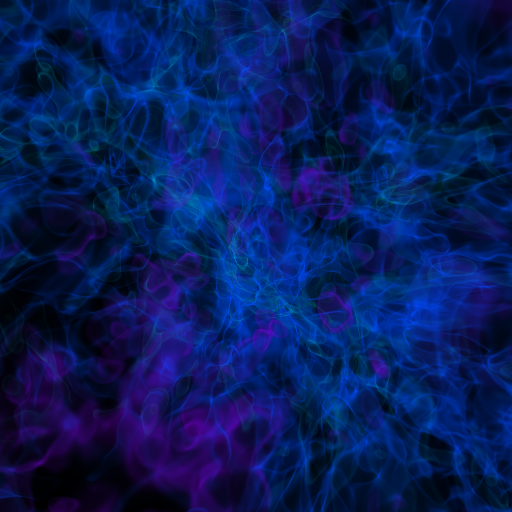
\includegraphics[scale=1.0]{./Visualization/yt_Nyx_density_vol_rend.png}
  \caption{Volume rendering of $128^3$ Nyx simulation using \yt. This
           corresponds to the same plot file used to generate the slice plot in
           Figure~\ref{fig:yt_Nyx_slice_plot}.}
  \label{fig:yt_Nyx_vol_rend}
\end{figure}

\subsection{Using \yt\ at NERSC (\emph{under development})}

Becase \yt\ is Python-based, it is portable and can be used in many software
environments. Here we focus on \yt's capabilities at NERSC, which provides
resources for performing both interactive and batch queue-based visualization
and analysis of \amrex\ data. Coupled with \yt's MPI and OpenMP parallelization
capabilities, this can enable high-throughput visualization and analysis
workflows.

\subsubsection{Interactive \yt\ with Jupyter notebooks}

Unlike \visit\ (\S\ref{sec:visit}), \yt\ has no client-server interface. Such
an interface is often crucial when one has large data sets generated on a
remote system, but wishes to visualize the data on a local workstation. Both
copying the data between the two systems, as well as visualizing the data
itself on a workstation, can be prohibitively slow.

Fortunately, NERSC has implemented several resources which allow one to
interact with \yt\ remotely, emulating a client-server model. In particular,
NERSC now hosts Jupyter notebooks which run IPython kernels on the Cori system;
this provides users access to the \texttt{\$HOME}, \texttt{/project}, and
\texttt{\$SCRATCH} file systems from a web browser-based Jupyter notebook.
\emph{\textbf{Please note that Jupyter hosting at NERSC is still under
development, and the environment may change without notice.}}

NERSC also provides Anaconda Python, which allows users to create their own
customizable Python environments. It is recommended to install \yt\ in such an
environment. One can do so with the following example:

\begin{lstlisting}
user@cori10:~> module load python/3.5-anaconda
user@cori10:~> conda create -p $HOME/yt-conda numpy
user@cori10:~> source activate $HOME/yt-conda
(/global/homes/u/user/yt-conda/) user@cori10:~> pip install yt
\end{lstlisting}

More information about Anaconda Python at NERSC is here:
\url{http://www.nersc.gov/users/data-analytics/data-analytics/python/anaconda-python/}.

One can then configure this Anaconda environment to run in a Jupyter notebook
hosted on the Cori system. Currently this is available in two places: on
\url{https://ipython.nersc.gov}, and on \url{https://jupyter-dev.nersc.gov}.
The latter likely reflects what the stable, production environment for Jupyter
notebooks will look like at NERSC, but it is still under development and
subject to change. To load this custom Python kernel in a Jupyter notebook,
follow the instructions at this URL under the ``Custom Kernels'' heading:
\url{http://www.nersc.gov/users/data-analytics/data-analytics/web-applications-for-data-analytics}.
After writing the appropriate \texttt{kernel.json} file, the custom kernel will
appear as an available Jupyter notebook. Then one can interactively visualize
\amrex\ plot files in the web browser.\footnote{It is convenient to use the
magic command \texttt{\%matplotlib inline} in order to render matplotlib
figures in the same browser window as the notebook, as opposed to displaying it
as a new window.}

\subsubsection{Parallel \yt}

Besides the benefit of no longer needing to move data back and forth between
NERSC and one's local workstation to do visualization and analysis, an
additional feature of \yt\ which takes advantage of the computational resources
at NERSC is its parallelization capabilities. \yt\ supports both MPI- and
OpenMP-based parallelization of various tasks, which are discussed here:
\url{http://yt-project.org/doc/analyzing/parallel_computation.html}.

Configuring \yt\ for MPI parallelization at NERSC is a more complex task than
discussed on the official \yt\ documentation; the command \texttt{pip install
mpi4py} is not sufficient. Rather, one must compile \texttt{mpi4py} from source
using the Cray compiler wrappers \texttt{cc}, \texttt{CC}, and \texttt{ftn} on
Cori. Instructions for compiling \texttt{mpi4py} at NERSC are provided here:
\url{http://www.nersc.gov/users/data-analytics/data-analytics/python/anaconda-python/#toc-anchor-3}.
After \texttt{mpi4py} has been compiled, one can use the regular Python
interpreter in the Anaconda environment as normal; when executing \yt\
operations which support MPI parallelization, the multiple MPI processes will
spawn automatically.

Although several components of \yt\ support MPI parallelization, a few are particularly useful:
\begin{itemize}
  \item \textbf{Time series analysis.} Often one runs a simulation for many
time steps and periodically writes plot files to disk for visualization and
post-processing. \yt\ supports parallelization over time series data via the
\texttt{DatasetSeries} object. \yt\ can iterate over a \texttt{DatasetSeries}
in parallel, with different MPI processes operating on different elements of
the series. This page provides more documentation:
\url{http://yt-project.org/doc/analyzing/time_series_analysis.html#time-series-analysis}.

  \item \textbf{Volume rendering}. \yt\ implements spatial decomposition among
MPI processes for volume rendering procedures, which can be computationally
expensive. Note that \yt\ also implements OpenMP parallelization in volume
rendering, and so one can execute volume rendering with a hybrid MPI+OpenMP
approach. See this URL for more details:
\url{http://yt-project.org/doc/visualizing/volume_rendering.html?highlight=openmp#openmp-parallelization}.

  \item \textbf{Generic parallelization over multiple objects.} Sometimes one
wishes to loop over a series which is not a \texttt{DatasetSeries}, e.g.,
performing translational or rotational operations on a camera to make a volume
rendering in which the field of view moves through the simulation. In this
case, one is applying a set of operations on a single object (a single plot
file), rather than over a time series of data. For this workflow, \yt\ provides
the \texttt{parallel\_objects()} function. See this URL for more details:
\url{http://yt-project.org/doc/analyzing/parallel_computation.html#parallelizing-over-multiple-objects}.

An example of MPI parallelization in \yt\ is shown below, where one animates a
time series of plot files from an IAMR simulation while revolving the camera
such that it completes two full revolutions over the span of the animation:

\begin{lstlisting}[language=python,breaklines=true]
import yt
import glob
import numpy as np

yt.enable_parallelism()

base_dir1 = '/global/cscratch1/sd/user/Nyx_run_p1'
base_dir2 = '/global/cscratch1/sd/user/Nyx_run_p2'
base_dir3 = '/global/cscratch1/sd/user/Nyx_run_p3'

glob1 = glob.glob(base_dir1 + '/plt*')
glob2 = glob.glob(base_dir2 + '/plt*')
glob3 = glob.glob(base_dir3 + '/plt*')

files = sorted(glob1 + glob2 + glob3)

ts = yt.DatasetSeries(files, parallel=True)

frame = 0
num_frames = len(ts)
num_revol = 2

slices = np.arange(len(ts))

for i in yt.parallel_objects(slices):
    sc = yt.create_scene(ts[i], lens_type='perspective', field='z_velocity')

    source = sc[0]
    source.tfh.set_bounds((1e-2, 9e+0))
    source.tfh.set_log(False)
    source.tfh.grey_opacity = False

    cam = sc.camera

    cam.rotate(num_revol*(2.0*np.pi)*(i/num_frames),
               rot_center=np.array([0.0, 0.0, 0.0]))

    sc.save(sigma_clip=5.0)
\end{lstlisting}

When executed on 4 CPUs on a Haswell node of Cori, the output looks like the following:

\begin{lstlisting}[breaklines=true]
user@nid00009:~/yt_vis/> srun -n 4 -c 2 --cpu_bind=cores python make_yt_movie.py
yt : [INFO     ] 2017-05-23 16:51:33,565 Global parallel computation enabled: 0 / 4
yt : [INFO     ] 2017-05-23 16:51:33,565 Global parallel computation enabled: 2 / 4
yt : [INFO     ] 2017-05-23 16:51:33,566 Global parallel computation enabled: 1 / 4
yt : [INFO     ] 2017-05-23 16:51:33,566 Global parallel computation enabled: 3 / 4
P003 yt : [INFO     ] 2017-05-23 16:51:33,957 Parameters: current_time              = 0.103169376949795
P003 yt : [INFO     ] 2017-05-23 16:51:33,957 Parameters: domain_dimensions         = [128 128 128]
P003 yt : [INFO     ] 2017-05-23 16:51:33,957 Parameters: domain_left_edge          = [ 0.  0.  0.]
P003 yt : [INFO     ] 2017-05-23 16:51:33,958 Parameters: domain_right_edge         = [ 6.28318531  6.28318531  6.28318531]
P000 yt : [INFO     ] 2017-05-23 16:51:33,969 Parameters: current_time              = 0.0
P000 yt : [INFO     ] 2017-05-23 16:51:33,969 Parameters: domain_dimensions         = [128 128 128]
P002 yt : [INFO     ] 2017-05-23 16:51:33,969 Parameters: current_time              = 0.0687808060674485
P000 yt : [INFO     ] 2017-05-23 16:51:33,969 Parameters: domain_left_edge          = [ 0.  0.  0.]
P002 yt : [INFO     ] 2017-05-23 16:51:33,969 Parameters: domain_dimensions         = [128 128 128]
P000 yt : [INFO     ] 2017-05-23 16:51:33,970 Parameters: domain_right_edge         = [ 6.28318531  6.28318531  6.28318531]
P002 yt : [INFO     ] 2017-05-23 16:51:33,970 Parameters: domain_left_edge          = [ 0.  0.  0.]
P002 yt : [INFO     ] 2017-05-23 16:51:33,970 Parameters: domain_right_edge         = [ 6.28318531  6.28318531  6.28318531]
P001 yt : [INFO     ] 2017-05-23 16:51:33,973 Parameters: current_time              = 0.0343922351851018
P001 yt : [INFO     ] 2017-05-23 16:51:33,973 Parameters: domain_dimensions         = [128 128 128]
P001 yt : [INFO     ] 2017-05-23 16:51:33,974 Parameters: domain_left_edge          = [ 0.  0.  0.]
P001 yt : [INFO     ] 2017-05-23 16:51:33,974 Parameters: domain_right_edge         = [ 6.28318531  6.28318531  6.28318531]
P000 yt : [INFO     ] 2017-05-23 16:51:34,589 Rendering scene (Can take a while).
P000 yt : [INFO     ] 2017-05-23 16:51:34,590 Creating volume
P003 yt : [INFO     ] 2017-05-23 16:51:34,592 Rendering scene (Can take a while).
P002 yt : [INFO     ] 2017-05-23 16:51:34,592 Rendering scene (Can take a while).
P003 yt : [INFO     ] 2017-05-23 16:51:34,593 Creating volume
P002 yt : [INFO     ] 2017-05-23 16:51:34,593 Creating volume
P001 yt : [INFO     ] 2017-05-23 16:51:34,606 Rendering scene (Can take a while).
P001 yt : [INFO     ] 2017-05-23 16:51:34,607 Creating volume
\end{lstlisting}

Because the \texttt{parallel\_objects()} function transforms the loop into a
data-parallel problem, this procedure strong scales nearly perfectly to an
arbitrarily large number of MPI processes, allowing for rapid rendering of
large time series of data.

\end{itemize}


\chapter{Profiling}\label{Chap:Profiling}
\amrex-based application codes can be instrumented using AMReX-specific performance
profiling tools that take into account the hierarchical nature of the mesh in 
most AMReX-based applications.  These codes can be instrumented for varying levels of 
profiling detail.  The broad-brush C++ instrumentation is as follows:

\section{Instrumenting the Code} 
\subsection{C++} 

\begin{lstlisting}[language=cpp]
void YourClass::YourFunction() 
{
  BL_PROFILE("YourClass::YourFunction()");  // this name can be any string

  // your function code
}
\end{lstlisting}

For other timers within an already instrumented function, add:
 
\begin{lstlisting}[language=cpp]
      BL_PROFILE_VAR("Flaten::FORT_FLATENX()", anyname);  // add this before
        FORT_FLATENX(arg1, arg2);
      BL_PROFILE_VAR_STOP(anyname);   // add this after, using the same name
\end{lstlisting}
 
if you want to use the same name within the same scope, you can use:
 
\begin{lstlisting}[language=cpp]
      BL_PROFILE_VAR("MyFuncs()", myfuncs);  // the first one
        MyFunc_0(arg);
      BL_PROFILE_VAR_STOP(myfuncs);
      ...
      BL_PROFILE_VAR_START(myfuncs);
        MyFunc_1(arg);
      BL_PROFILE_VAR_STOP(myfuncs);
\end{lstlisting}
 
or create a profiling variable without starting, then start/stop:
 
\begin{lstlisting}[language=cpp]
      BL_PROFILE_VAR_NS("MyFuncs()", myfuncs);  // dont start the timer
      ...
      BL_PROFILE_VAR_START(myfuncs);
        MyFunc_0(arg);
      BL_PROFILE_VAR_STOP(myfuncs);
      ...
      BL_PROFILE_VAR_START(myfuncs);
        MyFunc_1(arg);
      BL_PROFILE_VAR_STOP(myfuncs);
\end{lstlisting}

\subsection{Fortran90} 

Fortran90 functions can also be instrumented with the following calls:
 
\begin{lstlisting}[language=fortran]
call bl_proffortfuncstart("my_function")
...
call bl_proffortfuncstop("my_function")
\end{lstlisting}
 
Note that the start and stop calls must be matched and the profiling output will warn of any 
{\tt bl\_proffortfuncstart} calls that were not stopped with {\tt bl\_proffortfuncstop} calls
(in debug mode only).  You will need to add {\tt bl\_proffortfuncstop}
before any returns and at the end of the function or at the point in the
function you want to stop profiling. 

\section{Types of Profiling} 

Currently you have two options for AMReX-specific profiling.  If you set {\tt TINY\_PROFILE = TRUE}
in your GNUMakefile then at the end of the run, a summary of exclusive and inclusive function times 
will be written to stdout.

If you set {\tt PROFILE = TRUE} then a {\tt bl\_prof} directory will be written that contains 
detailed per-task timings of the code.    An exclusive-only set of function timings will be written to stdout

If, in addition to  {\tt PROFILE = TRUE}, you set {\tt TRACE\_PROFILE = TRUE}, then the profiler keeps track
of when each profiled function is called and  the {\tt bl\_prof} directory will include the function call stack.   
This is especially useful when core functions, such as {\tt FillBoundary} can be called from many different regions of the code.
Part of the trace profiling is the ability to set regions in the code which can be analyzed for profiling information independently from other regions. 

If, in addition to  {\tt PROFILE = TRUE}, you set {\tt COMM\_PROFILE = TRUE}, then the {\tt bl\_prof} directory 
will contain additional information about MPI communication (point-to-point timings, data volume, barrier/reduction times, etc.).  {\tt TRACE\_PROFILE = TRUE} and {\tt COMM\_PROFILE = TRUE} can be set together.

The AMReX-specific profiling tools are currently under development and this documentation will reflect the latest 
status in the development branch.

\section{Sample Output}

Sample output from {\tt TINY\_PROFILE = TRUE} can look like the following:


\begin{lstlisting}[basicstyle=\tiny,tabsize=1]

TinyProfiler total time across processes [min...avg...max]: 1.765...1.765...1.765
---------------------------------------------------------------------------------
Name                          NCalls   Excl. Min   Excl. Avg   Excl. Max   Max  %
---------------------------------------------------------------------------------
mfix_level::EvolveFluid       1        1.602       1.668       1.691       95.83%
FabArray::FillBoundary()      11081    0.02195     0.03336     0.06617      3.75%
FabArrayBase::getFB()         22162    0.02031     0.02147     0.02275      1.29%
PC<...>::WriteAsciiFile()     1        0.00292     0.004072    0.004551     0.26%


---------------------------------------------------------------------------------
Name                          NCalls   Incl. Min   Incl. Avg  Incl. Max    Max  %
---------------------------------------------------------------------------------
mfix_level::Evolve()          1        1.69        1.723      1.734        98.23%
mfix_level::EvolveFluid       1        1.69        1.723      1.734        98.23%
FabArray::FillBoundary()      11081    0.04236     0.05485    0.08826       5.00%
FabArrayBase::getFB()         22162    0.02031     0.02149    0.02275       1.29%

\end{lstlisting}

\section{\tt AMRProfParser} 

{\tt AMRProfParser} is a tool for processing and analyzing the {\tt bl\_prof} database.  It is a
command line application that can create performance summaries, plotfiles showing
point to point communication and timelines, HTML call trees, communication call
statistics, function timing graphs, and other data products.  The parser's data
services functionality can be called from an interactive environment such as {\tt Amrvis},
from a sidecar for dynamic performance optimization, and from other utilities such as
the command line version of the parser itself.  It has been integrated into {\tt Amrvis}
for visual interpretation of the data allowing {\tt Amrvis} to open the {\tt bl\_prof} database
like a plotfile but with interfaces appropriate to profiling data. AMRProfParser
and {\tt Amrvis} can be run in parallel both interactively and in batch mode.



%\chapter{Debugging}\label{Chap:Debugging}
%On debugging

% , Floating-Point Exceptions, and Backtrace


\chapter{CVODE}\label{Chap:CVODE}
\amrex\ supports ODE integration using the \cvode\ solver,\footnote{\url{https://computation.llnl.gov/projects/sundials/cvode}} which is part of the \sundials\ framework.\footnote{\url{https://computation.llnl.gov/projects/sundials}}
\cvode\ contains solvers for stiff and non-stiff ODEs, and as such is well suited for solving e.g., the complex chemistry networks in combustion simulations, or the nuclear reaction networks in astrophysical simulations.

Most of \cvode\ is written in C, but many functions also come with two distinct Fortran interfaces.
One interface is \fcvode, which is bundled with the stable release of \cvode.
Its usage is described in the CVODE documentation (\url{https://computation.llnl.gov/sites/default/files/public/cv_guide.pdf}).

The second, newer Fortran interface to \cvode\ uses the \texttt{iso\_c\_binding} feature of the Fortran 2003 standard to implement a ``thinner,'' more direct interface to the C functions in \cvode.
In contrast to the \fcvode\ interface, the Fortran 2003 interface calls C functions directly, with identical arguments.
When compiling \cvode, one need not build the Fortran interface to \cvode\ at all to use this new interface.
The examples provided in \amrex\ use this new interface.

To use \cvode\ in an \amrex\ application, follow these steps:

\begin{enumerate}

  \item Obtain the \cvode\ source code, which is hosted here: \url{https://computation.llnl.gov/projects/sundials/sundials-software}.

  One can download either the complete \sundials\ package, or just the \cvode\ components.

  \item Unpack the \cvode/\sundials\ tarball, and create a new ``build'' directory (it can be anywhere).

  \item Navigate to the new, empty build directory, and type

  \begin{verbatim}
  cmake \
    -DCMAKE_INSTALL_PREFIX:PATH=/path/to/install/dir \
    /path/to/cvode/or/sundials/top/level/source/dir
  \end{verbatim}

  The \texttt{CMAKE\_INSTALL\_DIR} option tells CMake where to install the libraries.
  Note that CMake will attempt to deduce the compilers automatically, but respects certain environment variables if they are defined, such as \texttt{CC} (for the C compiler), \texttt{CXX} (for the C++ compiler), and \texttt{FC} (for the Fortran compiler).
  So one may modify the above CMake invocation to be something like the following:

  \begin{verbatim}
  CC=/path/to/gcc \
  CXX=/path/to/g++ \
  FC=/path/to/gfortran \
    cmake \
    -DCMAKE_INSTALL_PREFIX:PATH=/path/to/install/dir \
    /path/to/cvode/or/sundials/top/level/source/dir
  \end{verbatim}

  \item In the \texttt{GNUmakefile} for the \amrex\ application which uses the Fortran 2003 interface to \cvode, add \texttt{USE\_CVODE = TRUE}, which will compile the Fortran 2003 interfaces and link the \cvode\ libraries.
  Note that one must define the \texttt{CVODE\_LIB\_DIR} environment variable to point to the location where the libraries are installed.
\end{enumerate}


%------------------------------------------------------------------------------
\backmatter

% \renewcommand\bibname{References}
% \addcontentsline{toc}{chapter}{References}
% \bibliographystyle{plain}
% \bibliography{refs,Verification/verification,Gravity/gr}

%\cleardoublepage
%\phantomsection
%\addcontentsline{toc}{chapter}{Index}
%\printindex

\end{document}
